\documentclass[a4paper]{report} %draft:显示空白页,final:显示图片
\usepackage[utf8]{inputenc}
\usepackage[margin=1.25in]{geometry}
\usepackage[UTF8]{ctex} % 中文支持
\usepackage{listings}
\usepackage{xcolor}
\usepackage{tabularx} % 自适应宽度表格
\usepackage{array}    % 表格格式增强
\usepackage{booktabs} % 更漂亮的横线
\usepackage{hyperref}
\usepackage{amsmath, amssymb} % 数学符号支持
\usepackage{bm} % 粗体数学符号
\usepackage{graphicx} %插入图片的宏包
\usepackage{float} %设置图片浮动位置的宏包
\usepackage{subcaption}
\usepackage{multirow}   % 合并单元格
\usepackage{caption}    % 控制表格标题
\usepackage{enumitem}
% \renewcommand{\bibname}{} % 去掉参考文献标题

\hypersetup{
    colorlinks=true,
    linkcolor=black,
    filecolor=magenta,
    urlcolor=cyan
}

\newcommand{\enabstractname}{Abstract}
\newcommand{\cnabstractname}{摘要}
\newenvironment{enabstract}{%
  \par\Large
  \noindent\mbox{}\hfill{\bfseries \enabstractname}\hfill\mbox{}\par
  \vskip 2.5ex}{\par\vskip 2.5ex}
\newenvironment{cnabstract}{%
  \par\Large
  \noindent\mbox{}\hfill{\bfseries \cnabstractname}\hfill\mbox{}\par
  \vskip 2.5ex}{\par\vskip 2.5ex}

\definecolor{codegray}{gray}{0.98}
\definecolor{codepurple}{rgb}{0.58,0,0.82}
\lstdefinestyle{mystyle}{
    backgroundcolor=\color{codegray},   
    commentstyle=\color{gray},
    keywordstyle=\color{blue},
    numberstyle=\tiny\color{gray},
    stringstyle=\color{codepurple},
    basicstyle=\ttfamily\small,
    breaklines=true,                 
    captionpos=b,                    
    keepspaces=true,                 
    numbers=left,                    
    numbersep=5pt,                  
    showspaces=false,                
    showstringspaces=false,
    showtabs=false,                  
    tabsize=4
}
\lstset{style=mystyle, language=Python}

\setcounter{tocdepth}{1} 

\title{不同噪声调控下布朗粒子的热扩散特性实验}
\author{}
\date{\today}

%% 正文开始
\begin{document}
\maketitle

\begin{cnabstract}
\large
  
热力学基本规律在宏观体系中已得到广泛验证,但其在微观尺度下的适用性仍需深入探讨。
本实验以布朗运动为典型模型,研究不同噪声调控下布朗粒子的热扩散特性,探索微观粒子在非平衡环境中的统计行为与热力学响应。
通过构建集光学观测与电噪声操控于一体的实验系统,我们在不改变体系实际温度的前提下,引入外部可控电噪声场,
实现了对粒子表观扩散强度与有效温度的主动调控。
实验结果表明,通过施加高斯白噪声可显著增强粒子的扩散行为,验证了噪声作为一种“人工热浴”在模拟高温扩散效应中的有效性。
进一步地,我们建立了噪声调控下扩散系数与熵产生之间的关联,揭示了微观随机运动与热力学第二定律在非平衡条件下的内在一致性。
本研究不仅为突破传统温控瓶颈提供了新范式,也为在微观尺度验证热力学基本规律、深入理解非平衡态体系的输运与耗散机制提供了新的实验途径。

\par\textbf{关键字: } 布朗运动,噪声调控,有效温度
\end{cnabstract}

\newpage
\begin{enabstract}
\large
The basic laws of thermodynamics have been widely verified in the macro system, but its applicability at the micro scale still needs to be further explored.
Taking Brownian motion as a typical model, this experiment studies the thermal diffusion characteristics of Brownian particles under different noise control, and explores the statistical behavior and thermodynamic response of microscopic particles in non-equilibrium environment.
By constructing an experimental system integrating optical observation and electric noise control, we introduce an externally controllable electric noise field without changing the actual temperature of the system.
The active regulation of the apparent diffusion intensity and effective temperature of particles is realized.
The experimental results show that the diffusion behavior of particles can be significantly enhanced by applying Gaussian white noise, which verifies the effectiveness of noise as an "artificial hot bath" in simulating high temperature diffusion effect.
Furthermore, we establish the correlation between diffusion coefficient and entropy generation under noise control, and reveal the internal consistency between microscopic random motion and the second law of thermodynamics under non-equilibrium conditions.
This study not only provides a new paradigm for breaking through the bottleneck of traditional temperature control, but also provides a new experimental approach for verifying the basic laws of thermodynamics at the microscopic scale and deeply understanding the transport and dissipation mechanism of non-equilibrium systems.
\par\textbf{Keyword: } Brownian motion, Noise Manipulation, Effective Temperature
\end{enabstract}

\tableofcontents

\chapter{实验背景与目的}

\section{实验背景:不同噪声调控下布朗粒子的热扩散特性研究}

\subsection{布朗运动与热扩散:从观测到操控}
布朗运动(Brownian Motion)是悬浮在流体中的微小粒子所表现出的不规则、无规则的随机运动现象。该现象最早由植物学家布朗(Robert Brown)在1827年发现 \cite{brown1828}. 
在统计物理的框架下,布朗运动被视为粒子与流体分子不断碰撞的结果,是连接微观热力学与宏观扩散过程的重要桥梁。爱因斯坦在1905年通过理论分析给出了布朗运动的定量描述,将其与扩散系数联系起来,
并为分子理论提供了实验证据 \cite{einstein1905}。它是微观分子热运动与宏观粒子行为之间的桥梁。对布朗粒子扩散特性的研究,不仅为统计物理基本理论(如涨落耗散定理、爱因斯坦关系)提供了关键验证,也是现代胶体科学、软物质物理和生物物理研究的核心手段。
传统上,粒子的热扩散特性通过扩散系数 $D$ 来表征,其由爱因斯坦关系
\[
D = \frac{kT}{6\pi \eta r}
\]
决定,表明在体系粘度 $\eta$ 和粒子半径 $r$ 固定时,扩散强度唯一地由环境温度 $T$ 主导。

\subsection{调控热扩散的传统途径及其瓶颈}
长期以来,调控温度是改变粒子热扩散特性的唯一直接方法。若要增强扩散,则需对体系进行全局加热。然而,这种传统温控方法在实验中面临多重严峻挑战:

\begin{enumerate}
  \item \textbf{应用局限}:许多生物、化学样品对温度极度敏感,高温会导致变性、失活或发生不必要的化学反应,限制了可研究的温度范围和样品类型。
  \item \textbf{引入干扰}:宏观加热易在样品池内形成温度梯度,从而触发对流,严重干扰对纯扩散运动的观测与分析,破坏了实验的准确性与可靠性。
  \item \textbf{响应迟缓}:热惯性的存在使得温度改变过程缓慢,难以实现扩散特性的快速、动态切换,无法满足某些需要高频调控的研究需求。
\end{enumerate}

这些瓶颈问题本质上源于温度作为一个全局、单一的热力学强度量的固有属性。因此,发展一种局部、快速、无损且强度可灵活编程的新方法来调控粒子的扩散行为,成为一个亟待解决的科学与技术问题。

\section{实验目的:构建光学观测与电噪声操控一体的实验系统}
布朗运动、扩散系数以及热噪声理论三者之间存在紧密联系。由此我们可以从统计物理的基本原理中找到突破口:根据涨落-耗散定理,布朗粒子的扩散行为本质上是由其所在环境的随机热力(即热噪声)所驱动的。
若能人为地引入一个与热噪声统计特性相似的可控外部随机力,便有可能在不改变体系实际温度的前提下,等效地调控粒子的扩散强度。换言之,我们可以通过设计一个“人工热浴”,来模拟或超越真实热环境的效果。
\subsection{噪声调控:一种突破瓶颈的新范式}
为突破物理温控的局限,本研究引入一种创新性的主动噪声调控。其核心思想是:通过施加一个外部的人工可控电噪声场,为布朗粒子提供一个额外的随机驱动力,从而模拟甚至超越热噪声的效果,最终实现对粒子表观扩散特性和有效温度的调控。

这种方法的理论基础在于朗之万方程所描述的粒子运动是各种随机力的线性叠加。一个外加的、与热噪声统计特性相似的电场力,可以直接贡献到粒子的均方位移中,从而等效地赋予粒子一个更高的“有效温度”($T_{\mathrm{eff}}$),使其表现出更强的扩散行为,即实现 $D_{\mathrm{eff}} \propto kT_{\mathrm{eff}} > kT$。

电噪声作为一种调控工具,具有无可比拟的优势:
\begin{itemize}
  \item \textbf{参数精确可调}:噪声的强度乃至统计分布均可通过信号发生器进行数字化精确设定与实时调整,为实现 “不同噪声调控” 研究提供了基础。
  \item \textbf{作用快速局部}:电场调控响应速度极快(可达微秒级),且通过微电极可实现高度空间局域化的操控,有效避免了全局加热的副作用。
  \item \textbf{非侵入与普适性}:该方法不改变介质的实际温度,对样品无损,适用于多种胶体颗粒体系。
\end{itemize}
基于上述背景,本实验报告旨在系统地开展“不同噪声调控下布朗粒子的热扩散特性”研究。我们将构建一个集光学观测与电噪声操控于一体的实验系统,核心研究内容包括:\\
1.证明实验材料进行的是布朗运动,即均方位移与时间间隔具有线性关系。\\
2.通过加载高斯白噪声,证明通过施加电压能够提高有效温度,探索其作为一种新型“力学热浴”的潜力,为在常温环境下模拟高温扩散效应、研究随机系统的输运性质提供一种全新的实验方法,填补大学物理实验中热学相关部分的空白。

\chapter{实验原理}
实验原理的推导工作主要围绕布朗粒子在外部随机驱动下的有效动能温度与扩散特性展开。\par
首先,在\textbf{有效动能温度公式推导}中,通过朗之万方程出发,分析了热噪声与附加随机噪声的共同作用。
结果表明,外加噪声项会等效提高粒子的动能温度,给出修正后的公式
\[
T_{\text{kin}} = T_w + \frac{\sigma^2}{2k\gamma},
\]
其中温度增量正比于噪声强度的平方,反比于阻尼系数。这一结论直接刻画了外部驱动对系统非平衡涨落的影响,
与实验研究中利用附加噪声调控布朗粒子温度的思路相吻合 \cite{Martinez2013,Roldan2014}。\par
随后,在\textbf{噪声强度与扩散系数的修正关系}部分,从过阻尼朗之万方程出发,将外部噪声纳入扩散系数的定义,得到
\[
D = \frac{k_B T_w}{\gamma} + \frac{\sigma^2}{2\gamma^2} = \mu k_B T_w + \frac{\sigma^2 \mu^2}{2},
\]
其中 $\mu = 1/\gamma$ 为迁移率。该结果揭示了非热噪声会额外贡献一个正的扩散项,从而改变系统的弛豫与熵产生率的下界估计。结合近期提出的熵产生率推导框架 \cite{Leighton2024},
这一修正有助于在广义随机热力学下刻画非平衡驱动的系统。\par
综上,本部分推导的目的在于建立一个统一的描述:通过在动能温度和扩散系数中引入外部随机力修正项,可以更准确地刻画布朗体系在非平衡条件下的动力学特征。
这既为实验测量与调控提供了理论依据 \cite{Martinez2013,Roldan2014},也与最新的熵产生率界限理论 \cite{Leighton2024} 相呼应。

\section{有效动能温度公式推导}

在研究布朗粒子非平衡涨落性质时,一个核心问题是如何合理地定义和刻画粒子的\textbf{有效动能温度}。
当粒子被光阱约束时,其运动可由朗之万方程描述。为了突出外部噪声对动能涨落的影响,这里采用自由粒子近似,忽略势能项。
动力学方程写为
\begin{equation}
m \frac{dv}{dt} = -\gamma v + \xi(t) + \zeta(t),
\end{equation}
其中摩擦力 $-\gamma v$ 描述粒子与流体环境之间的黏滞阻尼,$\xi(t)$ 是来自热浴的随机噪声,对应环境温度 $T_w$,
而 $\zeta(t)$ 表示由外加电场或其他方式引入的外部随机力,幅值为 $\sigma$。  
对于噪声项,通常假设其为高斯白噪声,具有零均值和 $\delta$ 相关性质。热噪声满足
\begin{equation}
\langle \xi(t) \xi(t') \rangle = 2\gamma k_B T_w \delta(t - t'),
\end{equation}
而外部随机力的相关函数为
\begin{equation}
\langle \zeta(t) \zeta(t') \rangle = \sigma^2 \delta(t - t'),
\end{equation}
二者相互独立,因此互相关为零。 \par 

定义总噪声 $\eta(t) = \xi(t) + \zeta(t)$,其统计特性可写为
\begin{equation}
\langle \eta(t)\eta(t') \rangle = \big( 2\gamma k_B T_w + \sigma^2 \big)\delta(t - t').
\end{equation}
这表明外部噪声的引入相当于在热噪声的基础上增加了一项有效的能量输入,从而改变系统的温度特征。  

朗之万方程的稳态解为
\begin{equation}
v(t) = \frac{1}{m} \int_{-\infty}^{t} e^{-\frac{\gamma}{m}(t-\tau)} \eta(\tau) \, d\tau,
\end{equation}
通过对其方差进行计算,可得
\begin{equation}
\langle v^2 \rangle = \frac{2\gamma k_B T_w + \sigma^2}{2\gamma m}.
\end{equation}

根据能量均分定理,动能与有效动能温度的关系为
\begin{equation}
\frac{1}{2} m \langle v^2 \rangle = \frac{1}{2} k_B T_{\text{kin}},
\end{equation}
代入上式便得到修正后的有效温度
\begin{equation}
T_{\text{kin}} = T_w + \frac{\sigma^2}{2k_B \gamma}.
\label{eq:Teff}
\end{equation}\par
这一结果揭示:\textbf{外部随机力会等效提高布朗粒子的有效动能温度}。其增加量与噪声强度平方 $\sigma^2$ 成正比,与摩擦系数 $\gamma$ 成反比。
这一现象已在实验中得到验证,例如 Martínez 等 \cite{Martinez2013} 利用电场噪声显著提高了布朗球的动能温度,Roldán 等 \cite{Roldan2014}
进一步将其应用于非平衡过程的能量测量。上述理论公式为理解和解释这些实验结果提供了坚实的基础。
\section{噪声强度与扩散系数的修正关系}\par

除了动能温度,外部随机力还会显著影响布朗粒子的扩散行为。为此,我们转而考虑过阻尼近似下的朗之万方程:
\begin{equation}
\gamma \dot{x} = f(x,t) + \eta(t),
\end{equation}
其中 $\eta(t)$ 的相关函数包含了热噪声和外部噪声的贡献:
\begin{equation}
\langle \eta(t)\eta(t') \rangle = \big( 2\gamma k_B T_w + \sigma^2 \big)\delta(t-t').
\end{equation}
根据随机微分方程理论,扩散系数定义为
\begin{equation}
D = \frac{2\gamma k_B T_w + \sigma^2}{2\gamma^2}.
\end{equation}
将其展开为两部分:
\begin{equation}
D = \frac{k_B T_w}{\gamma} + \frac{\sigma^2}{2\gamma^2}.
\end{equation}
第一项是标准的 Einstein 关系,描述由热噪声引起的扩散;第二项则是外部噪声的修正,说明附加的随机驱动能够显著增强系统的扩散强度。
若进一步引入迁移率 $\mu = 1/\gamma$,则可写为
\begin{equation}
D = \mu k_B T_w + \frac{\sigma^2 \mu^2}{2}.
\label{eq:erciguanxi}
\end{equation}\par
量纲分析表明,该公式在物理上自洽。非热噪声项 $\sigma^2/(2\gamma^2)$ 的单位确实与扩散系数相符,即 $\mathrm{m^2/s}$。  
在此基础上,概率流与熵产生率的公式可保持原有定义:
\begin{equation}
J(x,t) = \mu f(x,t)p(x,t) - D \partial_x p(x,t),
\end{equation}
\begin{equation}
\dot{\Sigma} = \frac{1}{D} \left\langle \left( \frac{J}{p} \right)^2 \right\rangle \geq \frac{\langle \dot{x} \rangle^2}{D}.
\end{equation}
与传统热噪声情形相比,此处的熵产生率界限受 $\sigma^2$ 修正后的扩散系数影响,从而在理论层面上与最新的熵产生下界理论(如 Leighton 和 Sivak 提出的 Jensen bound \cite{Leighton2024})形成呼应。\par  
本节结果不仅为非平衡布朗动力学提供了更全面的刻画,还为实验上通过外场调控噪声强度进而控制扩散与熵产生提供了理论依据。

\chapter{理论模拟}
在进行实验之前,我们首先需要验证理论推导的正确性。考虑到本实验预期的最终结果我们的理论模拟部分包括:

\begin{enumerate}
  \item 均方位移(MSD)与时间 $t$ 的线性关系验证:聚苯乙烯(PS)微球在溶液中应当做布朗运动。对于布朗运动粒子,其均方位移(MSD)应当与时间 $t$ 呈线性关系,因此可将该关系作为判断 PS 微球是否进行布朗运动的依据。

  \item 朗之万方程数值模拟与等效温度:当外加噪声电压时,需要模拟在电噪声驱动下 PS 微球的运动是否仍然保持与布朗运动相似的性质。为此,我们基于朗之万方程进行了数值模拟,并计算了等效温度。

  \item 不同 $\sigma$ 下的扩散系数拟合:最后,我们对前文的关系式~\eqref{eq:erciguanxi} 进行了数值验证,证明模拟结果与理论计算的预期一致。
\end{enumerate}
\newpage
\section{ MSD 与时间 $t$ 的线性关系验证}

对于一个直径 $0.5~\mu\text{m}$ 的粒子,在 $20^\circ$C 水溶液中做布朗运动时,其轨迹如图所示:
\begin{figure}[H]
  \centering
  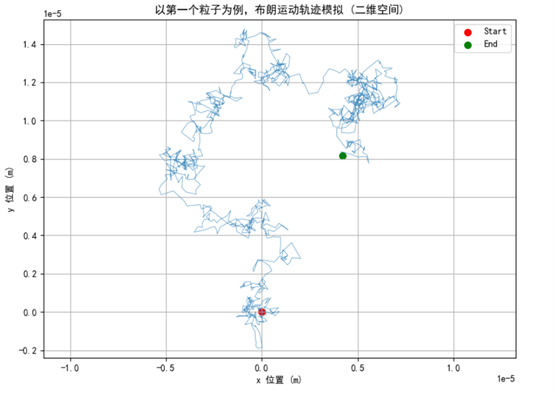
\includegraphics[width=0.7\textwidth]{trajectory.png}
  \caption{直径 $0.5~\mu$m 粒子的布朗运动轨迹示意}
  \label{fig:trajectory}
\end{figure}

我们主要探究粒子在一维方向的运动特性。以其中 3 个粒子为例,其一维方向的位移随时间变化如图所示:
\begin{figure}[H]
  \centering
  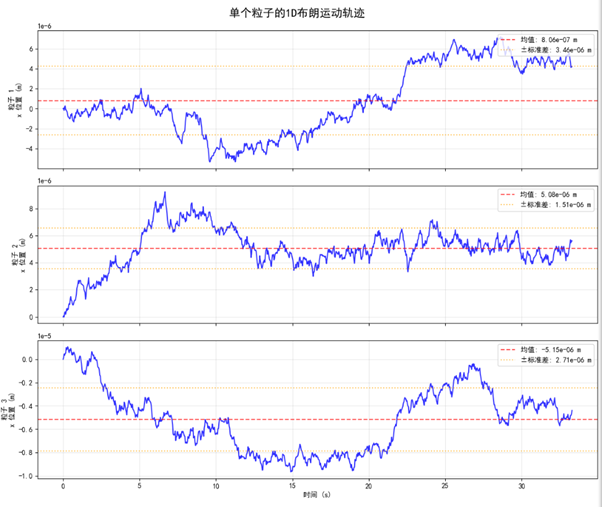
\includegraphics[width=0.8\textwidth]{displacement.png}
  \caption{三颗粒子在一维方向的位移随时间变化}
  \label{fig:displacement}
\end{figure}
将模拟粒子运动的二维MSD与上述理论绘制成图进行对比可以得到:
\begin{figure}[H]
  \centering
  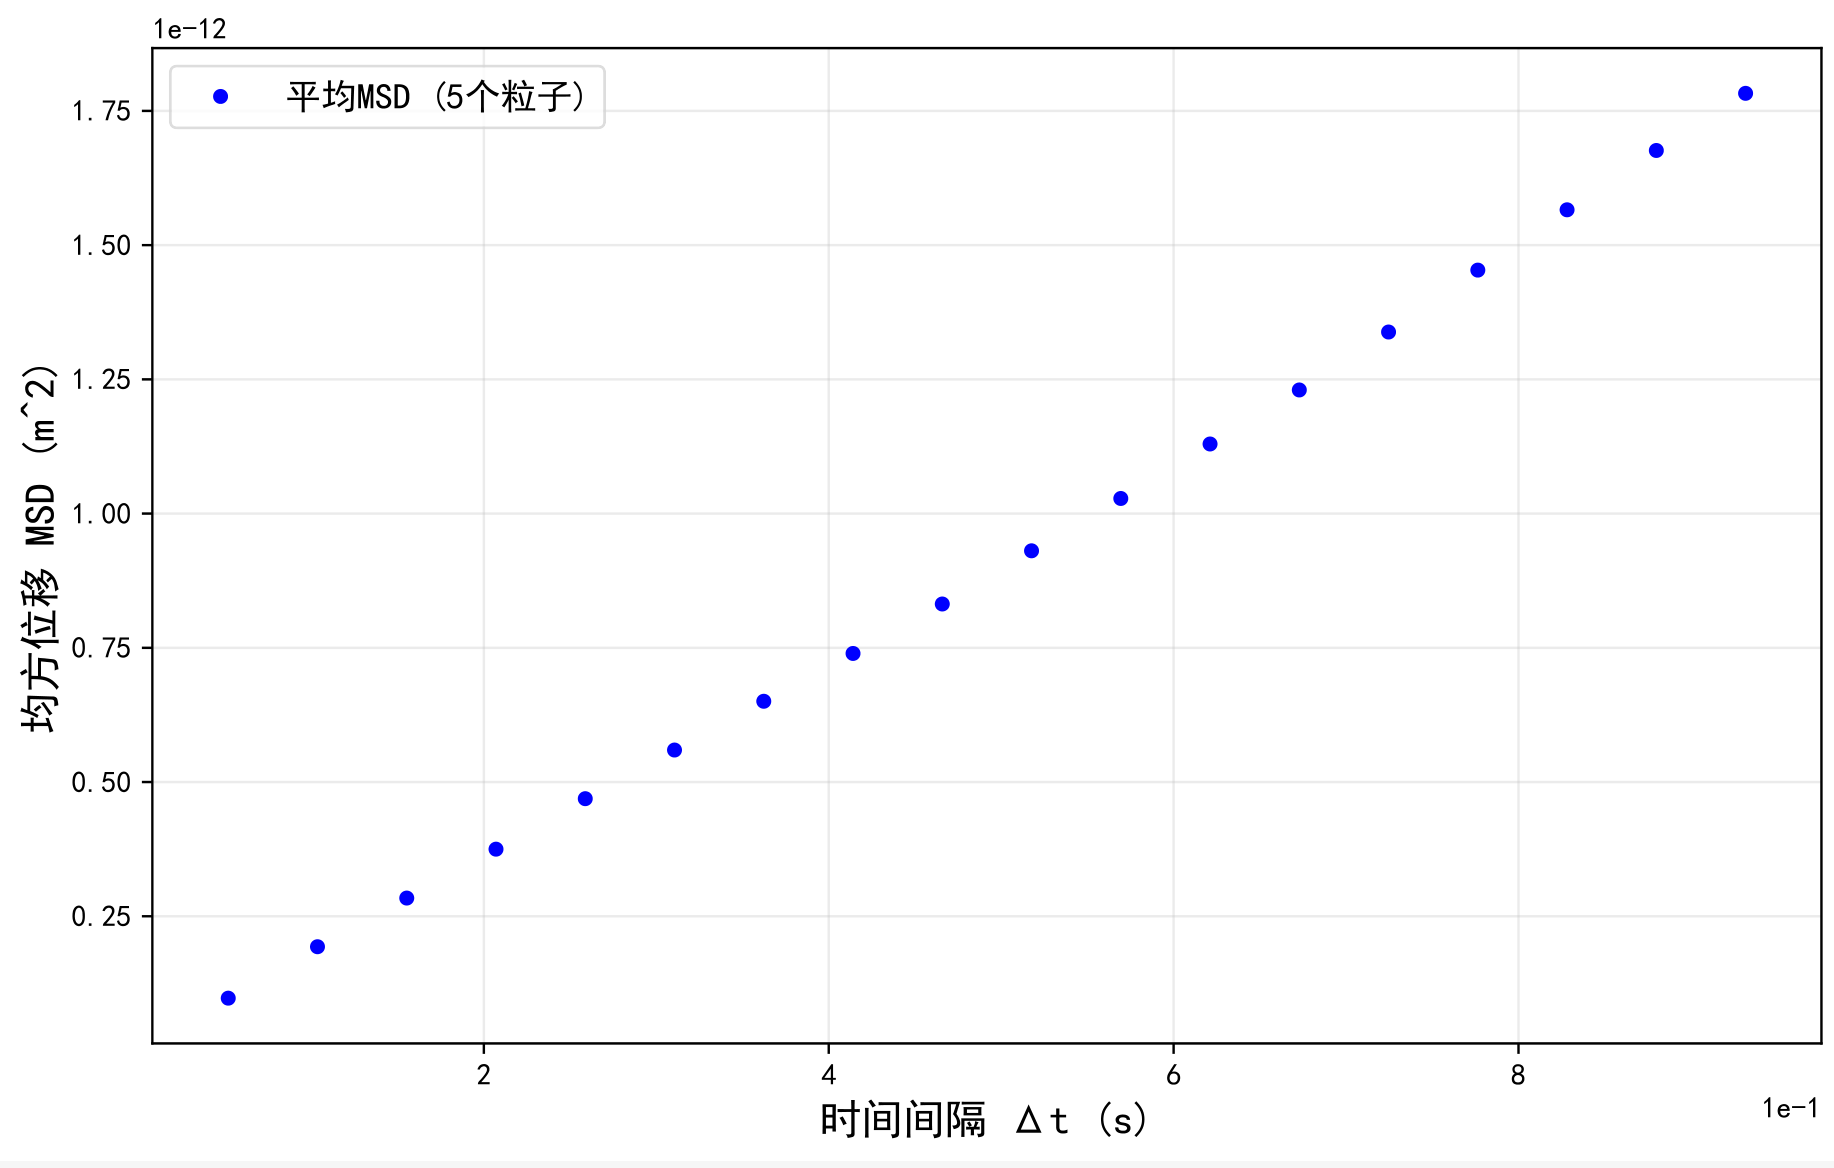
\includegraphics[width=0.8\textwidth]{二维MSD.png}
  \caption{直径$0.5~\mu\text{m}$二维MSD理论与模拟}
\end{figure}
对于多个 $0.5~\mu\text{m}$ 的粒子,在 $20^\circ$C 水溶液中做布朗运动时,其总 MSD 与时间满足\cite{einstein1905}:
\begin{align}
  \text{MSD}(t) &= 2Dt \quad &\text{(一维)} \\
  \text{MSD}(t) &= 4Dt \quad &\text{(二维)}
\end{align}
可以看到我们的理论在模拟上是正确的,可以作为判定PS微球是否进行布朗运动的依据

\section{朗之万方程数值模拟与等效温度}
\subsection{噪声对布朗运动的影响}

若在溶液环境中引入白噪声电场力,其作用可通过附加一项随机力 $\xi(t)$ 表示。对于直径 $0.5~\mu\text{m}$ 的粒子,随机电场力振幅 $\sigma$ 的定义为
\begin{equation}
  \sigma = q \frac{V_0}{d},
\end{equation}
其中,$q$ 为粒子所带电荷量,$V_0$ 为电极两端所加电压,$d$ 为电极间距。实验中,$\sigma$ 的数量级约为 $10^{-14}$,$d = 0.02~\text{m}$,$q \approx 10^{-16}$,因此 $V_0$ 设置在 $1$--$10~\text{V}$ 范围内。

在该条件下,粒子的有效温度会升高,但其 $x$ 方向位移依旧表现出一维随机布朗运动的性质。我们对该情况下的粒子运动也进行了模拟:
\begin{figure}[H]
  \centering
  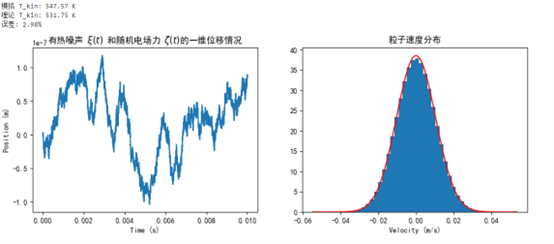
\includegraphics[width=0.9\textwidth]{一维位移.png}
  \caption{加噪声情况下的粒子}
  \label{fig:一维位移}
\end{figure}
提取我们关注的一维信息后,得到了x随时间的变化图:
\begin{figure}[H]
  \centering
  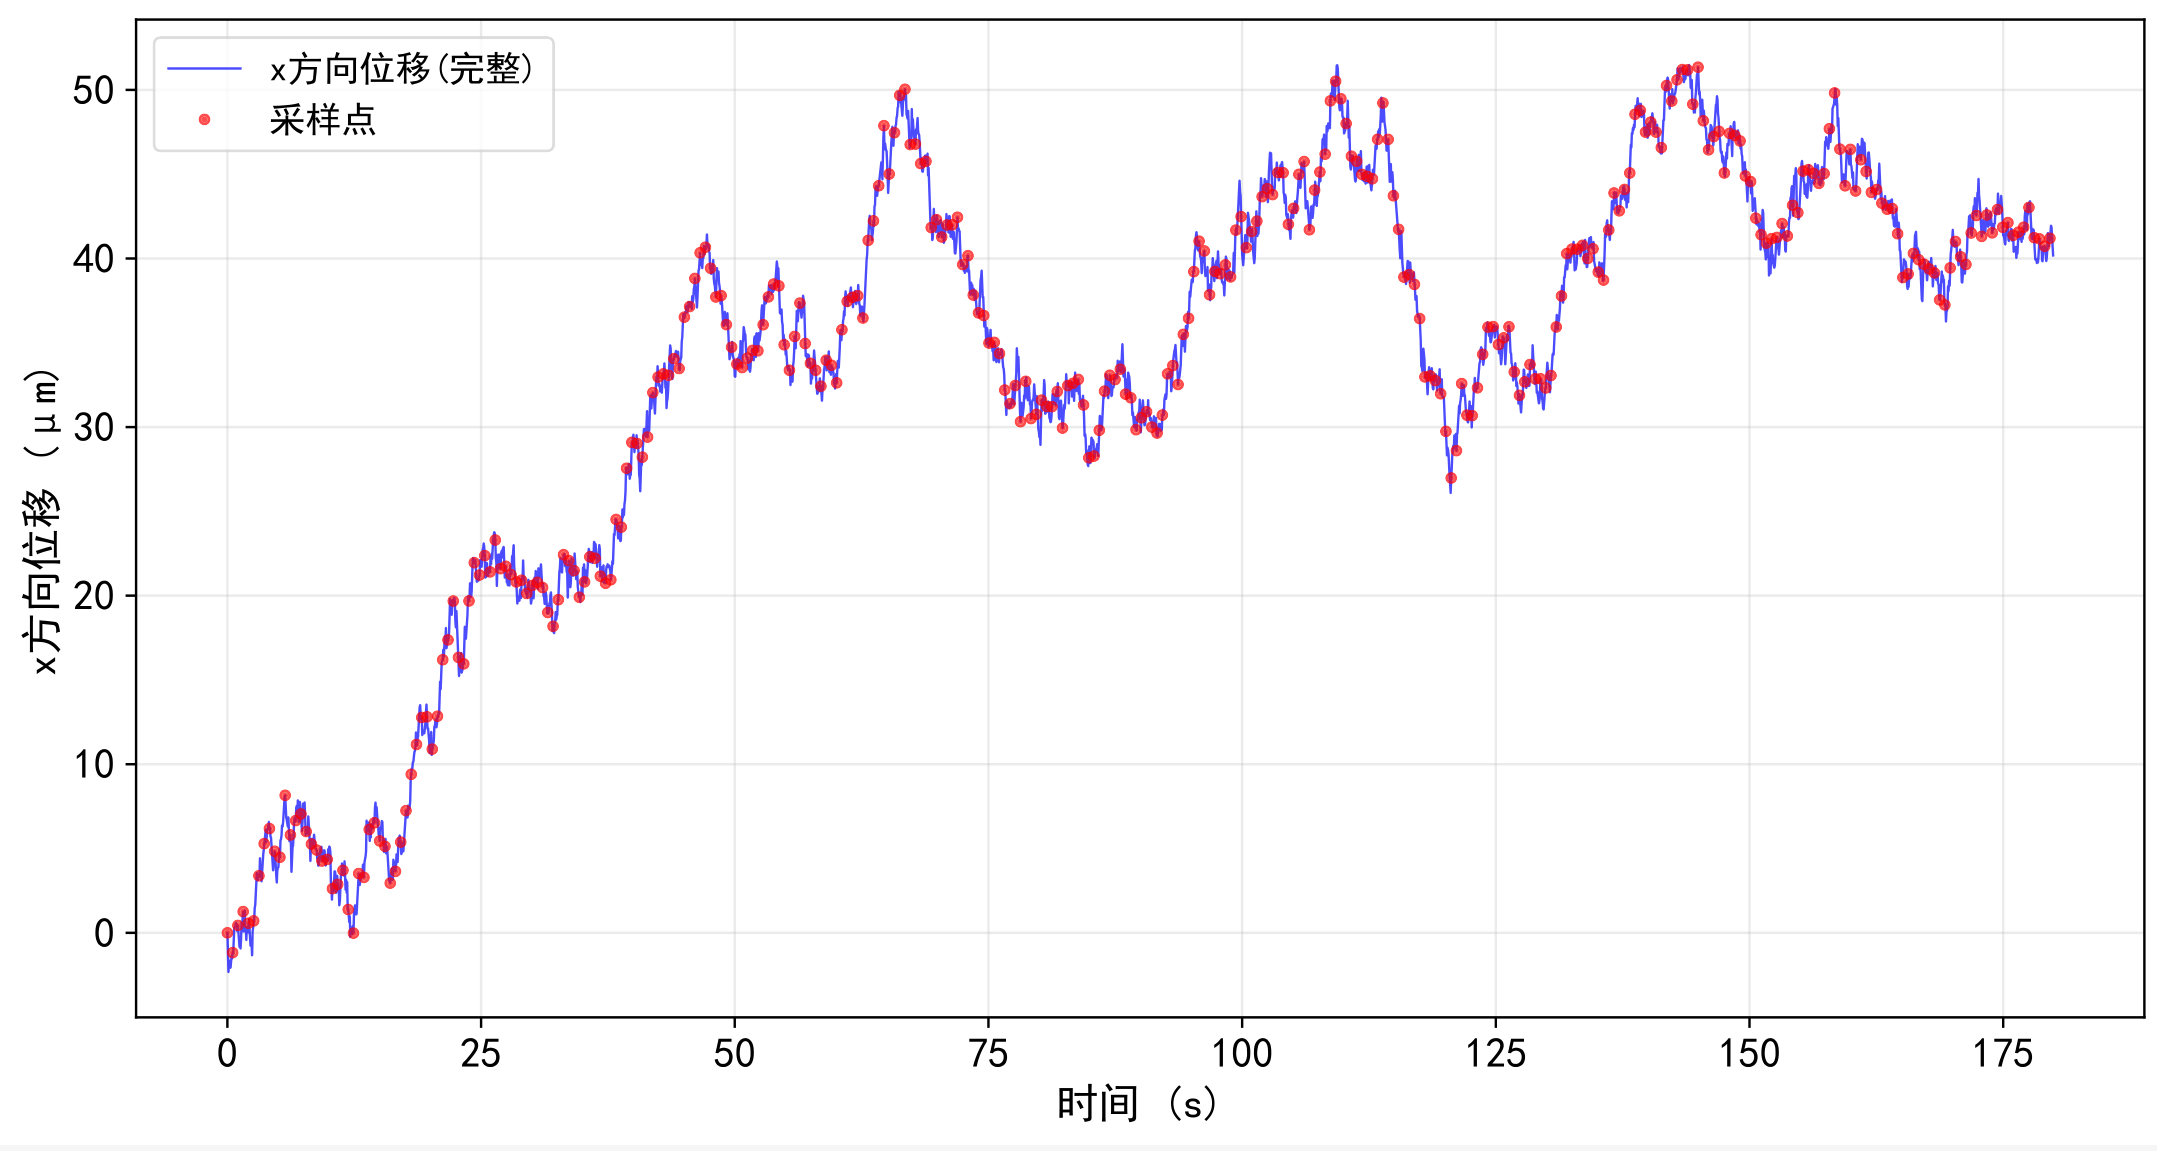
\includegraphics[width=0.9\textwidth]{x.png}
  \caption{一维情况下加噪声的粒子}
\end{figure}

布朗运动在一维情况下可由朗之万方程描述:
\begin{equation}
  m \frac{dv}{dt} = -\gamma v + \xi(t) + \zeta(t),
\end{equation}
其中,$\gamma$ 为摩擦系数,$\xi(t)$ 表示热噪声,$\zeta(t)$ 表示外加电噪声。根据能量均分定理,定义等效动能温度为
\begin{equation}
  T_{\text{eff}} = \frac{m \langle v^2 \rangle}{k_B},
\end{equation}
其中 $k_B$ 为玻尔兹曼常数,$m$ 为粒子质量,$\langle v^2 \rangle$ 为速度方差。

\section{不同 $\sigma$ 下的扩散系数拟合}

根据前面推导的方程\eqref{eq:erciguanxi},当引入噪声时,扩散系数随 $\sigma$ 的变化关系可表示为
\begin{equation}
  D = D_0 + k\sigma^2,
  \label{eq:D_sigma}
\end{equation}
其中 $D_0$ 为无外加噪声时的扩散系数,$k$ 为拟合系数。因此,$D$ 与 $\sigma$ 呈二次曲线关系。

\begin{figure}[H]
  \centering
  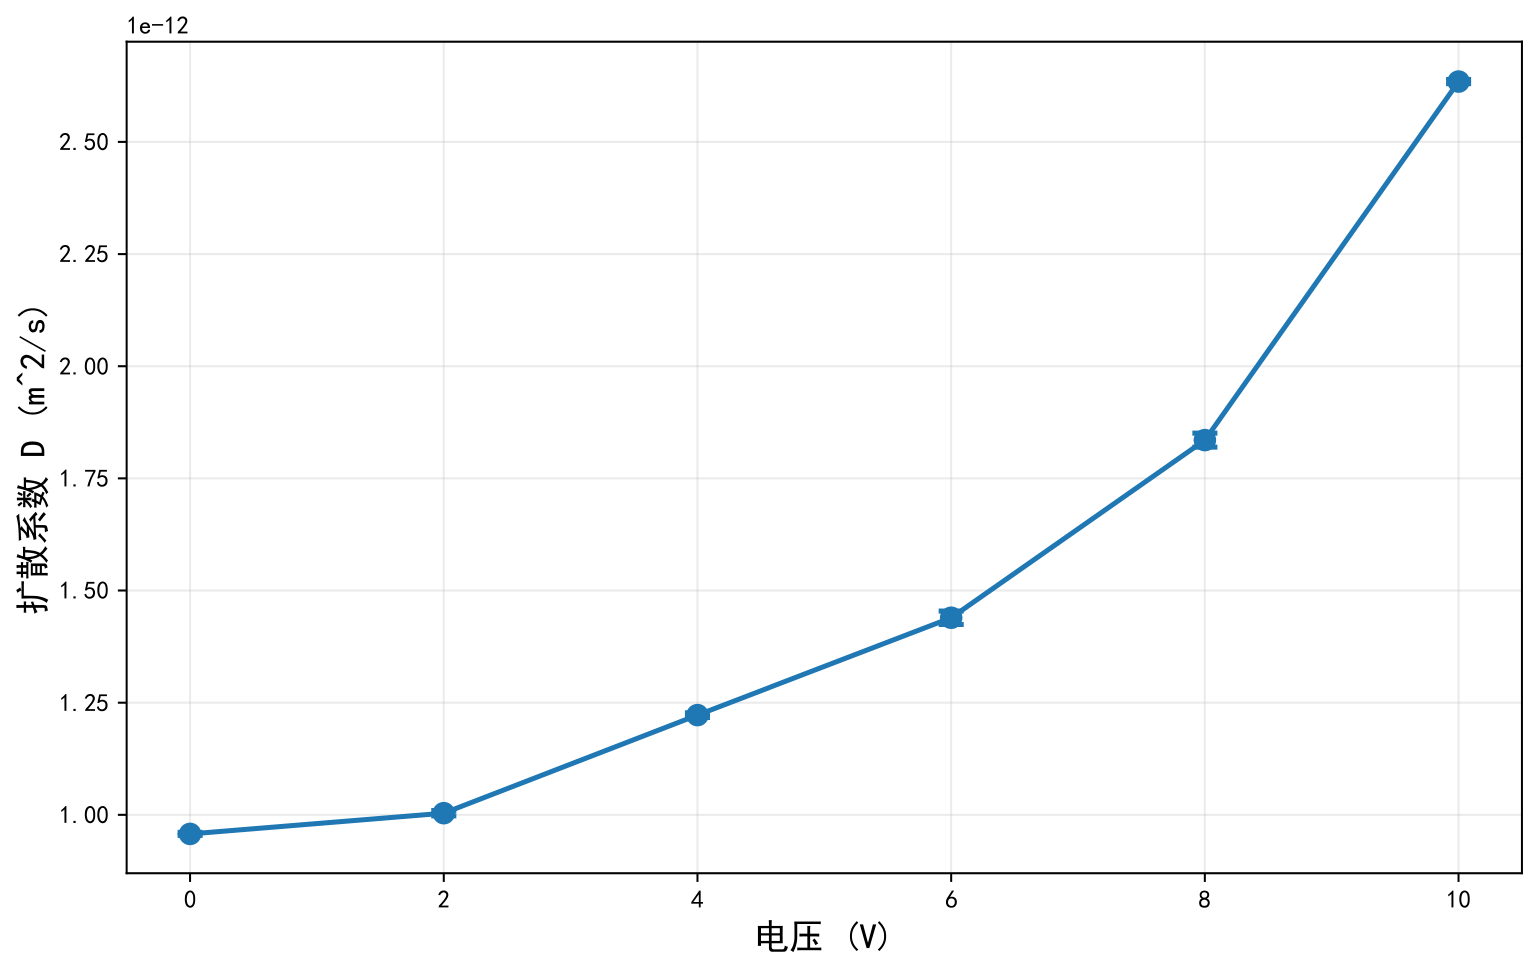
\includegraphics[width=0.8\textwidth]{fit.png}
  \caption{不同噪声强度下扩散系数 $D$ 的拟合结果}
  \label{fig:fit}
\end{figure}


\chapter{装置设计}
\section{实验仪器设计与创新点}
(1)由于水平放置的样品容易受到重力作用,悬浮粒子会逐渐沉降至样品底部,进而受到附加阻力的影响,导致微球的布朗运动减弱,
不利于作为理想的实验对象\cite{einstein1905,dhont1996brownian}。\par
本实验采用垂直放置样品的设计,以最大程度减小重力对粒子运动的干扰。垂直放置不仅能够更好地匹配显微镜的光学路径,
从而提升成像质量与分辨率,还能更准确地捕捉布朗粒子的运动轨迹。此外,该设计也便于电极的插入与固定,为后续加载噪声信号提供了实验条件。\par

(2)在光源选择方面,本实验采用非相干光源作为照明。相比于相干光,非相干光源具有较宽的光谱范围和较低的相干性,可有效抑制干涉和衍射效应,
从而提升成像的均匀性与清晰度,更适合布朗粒子的观测需求\cite{goodman,mandel1995optical}。\par

(3)对于噪声的引入,本实验利用信号发生器产生可控的电噪声信号。
通过调节其输出频率与幅度,可精确控制噪声特性,以适应不同实验条件\cite{horowitz1989art,schreiber1999electrical}。\par

(4)我们在理论上证明了可以通过加载电噪声的方式来等效地提高温度,为热学实验中的温度控制提供了一种新的,可行的,有效快速均匀地控制温度的方法。
\begin{figure}[H]
    \centering
    % 每行 4 张
    \begin{subfigure}{0.22\textwidth}
        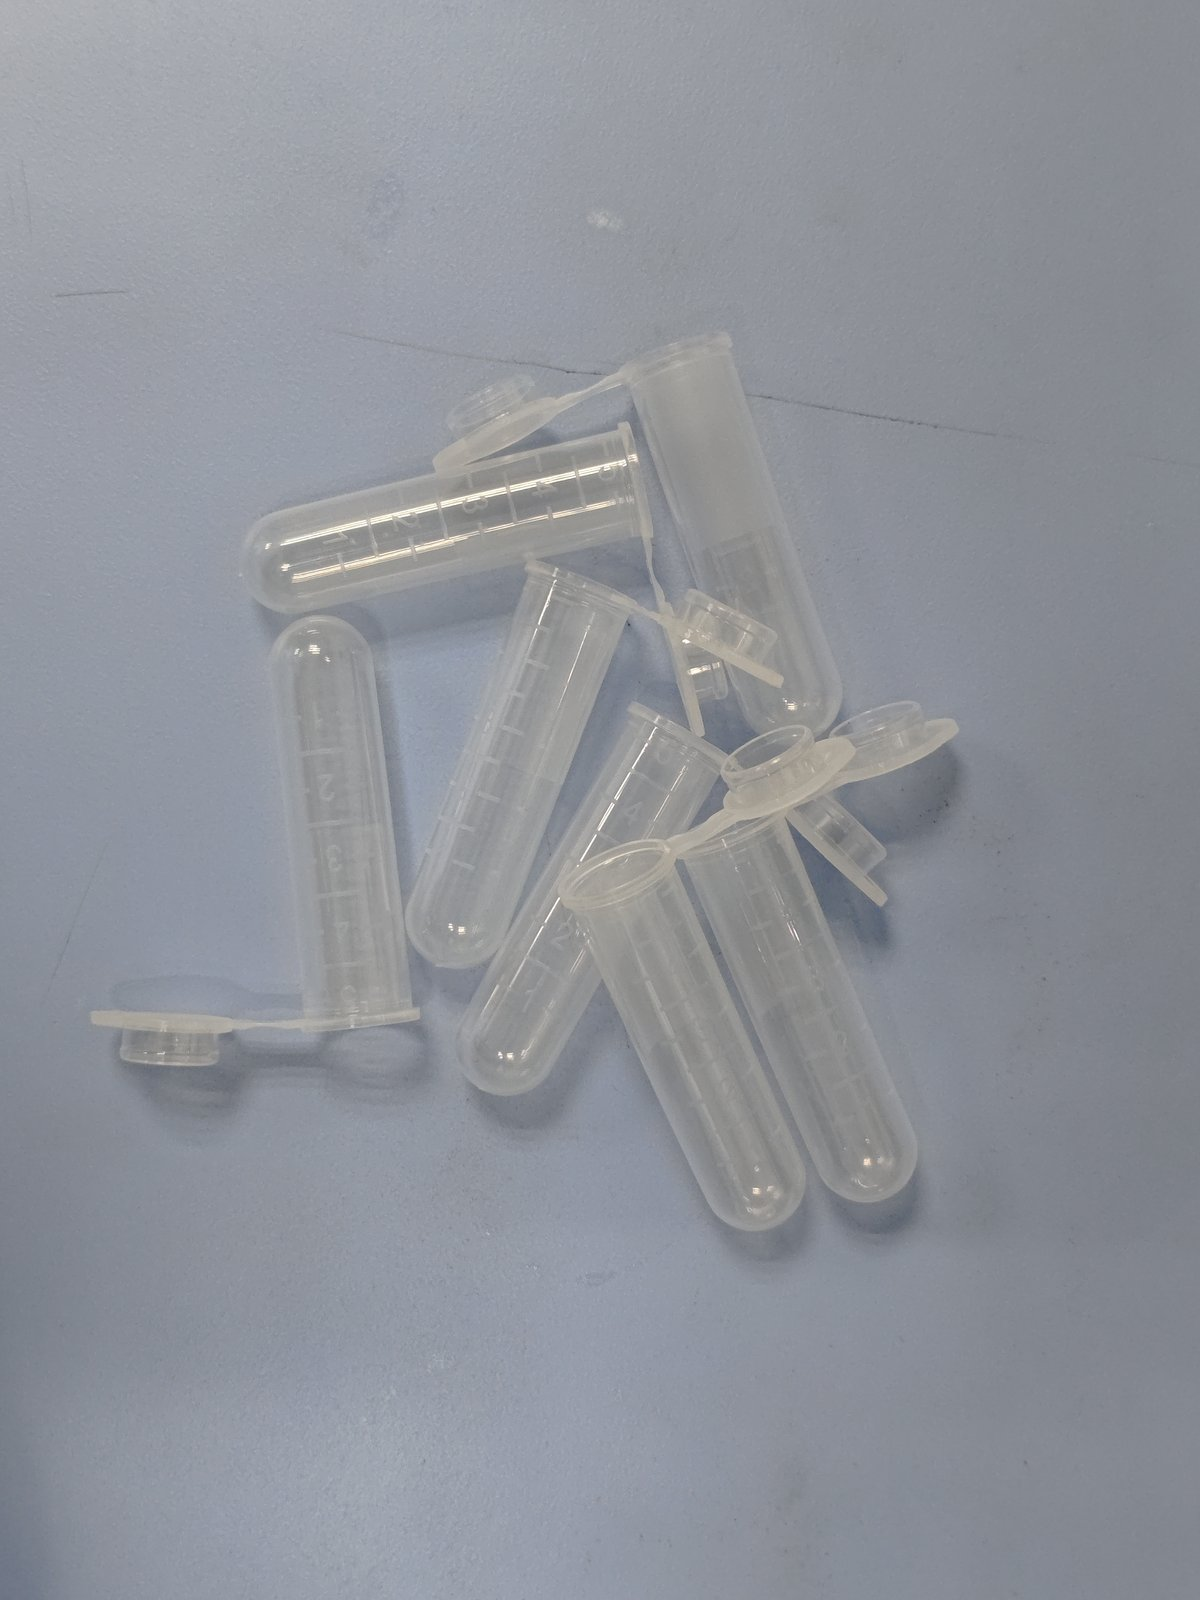
\includegraphics[width=\linewidth]{5.0ml微量离心管.jpg}
        \caption{5.0ml微量离心管}
    \end{subfigure}
    \begin{subfigure}{0.22\textwidth}
        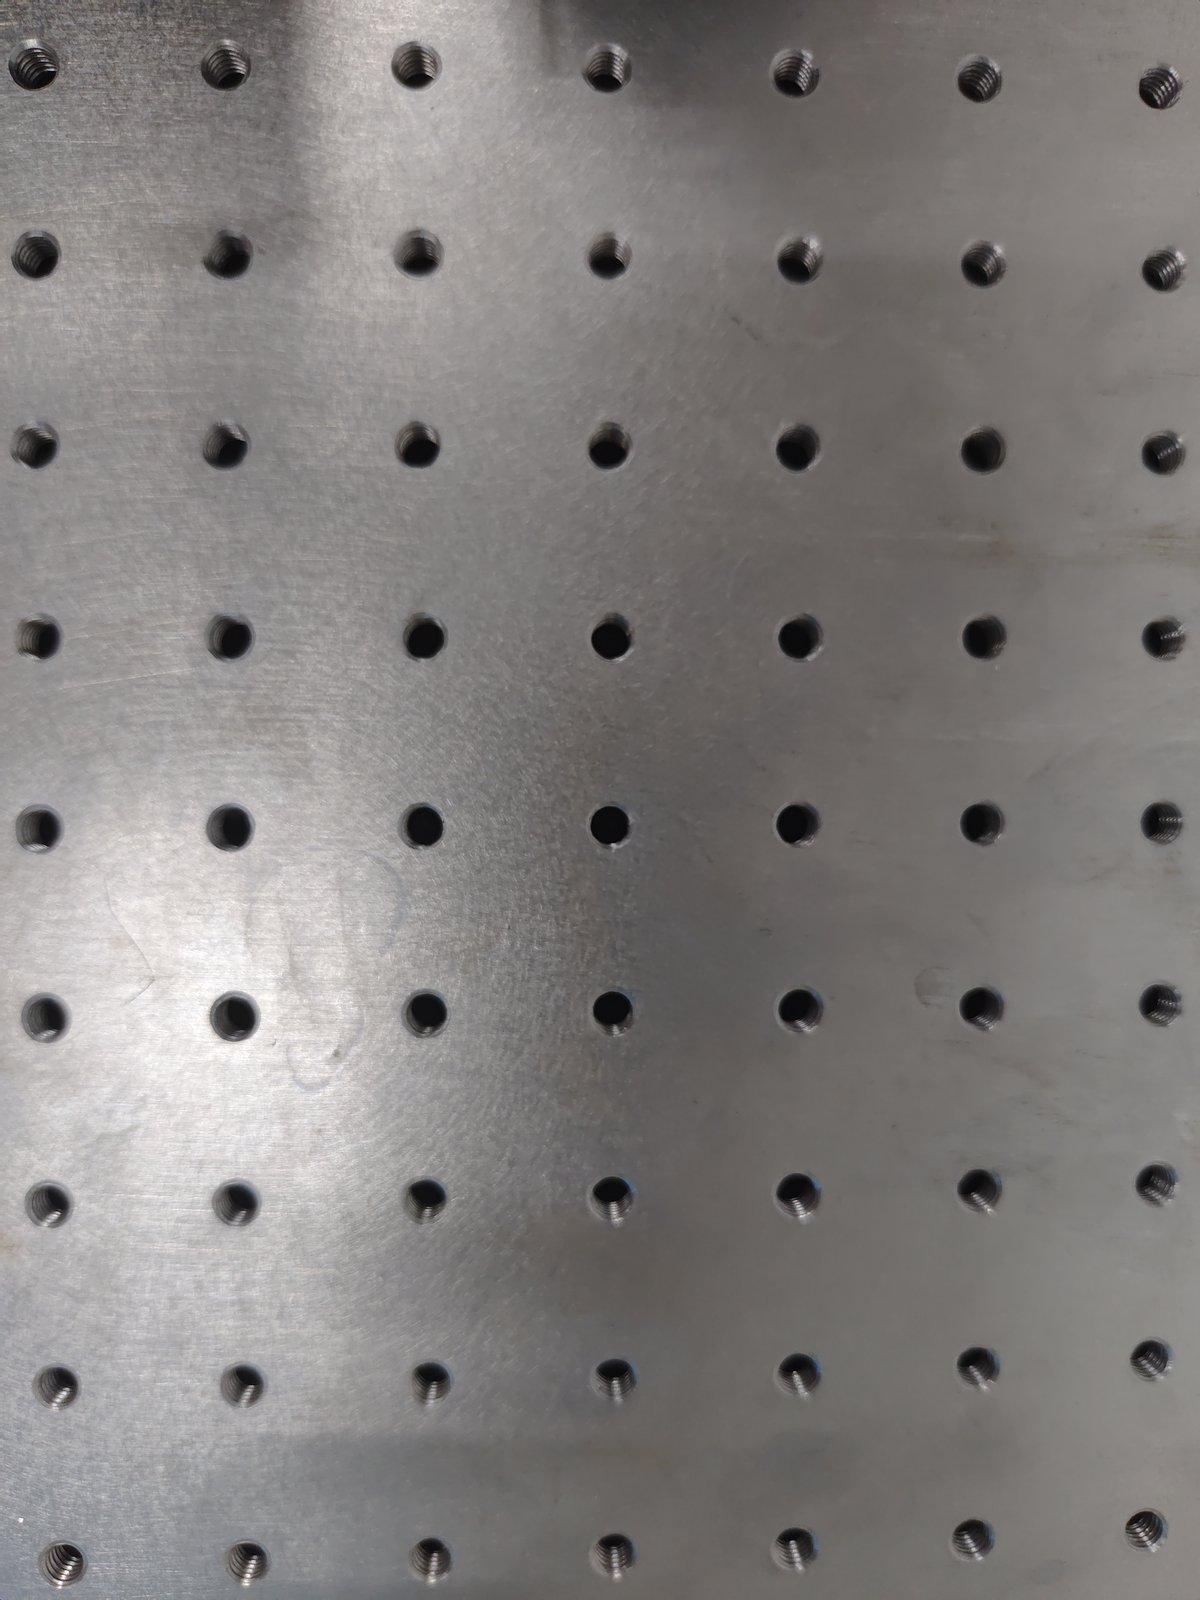
\includegraphics[width=\linewidth]{光学平台.jpg}
        \caption{光学平台}
    \end{subfigure}
    \begin{subfigure}{0.22\textwidth}
        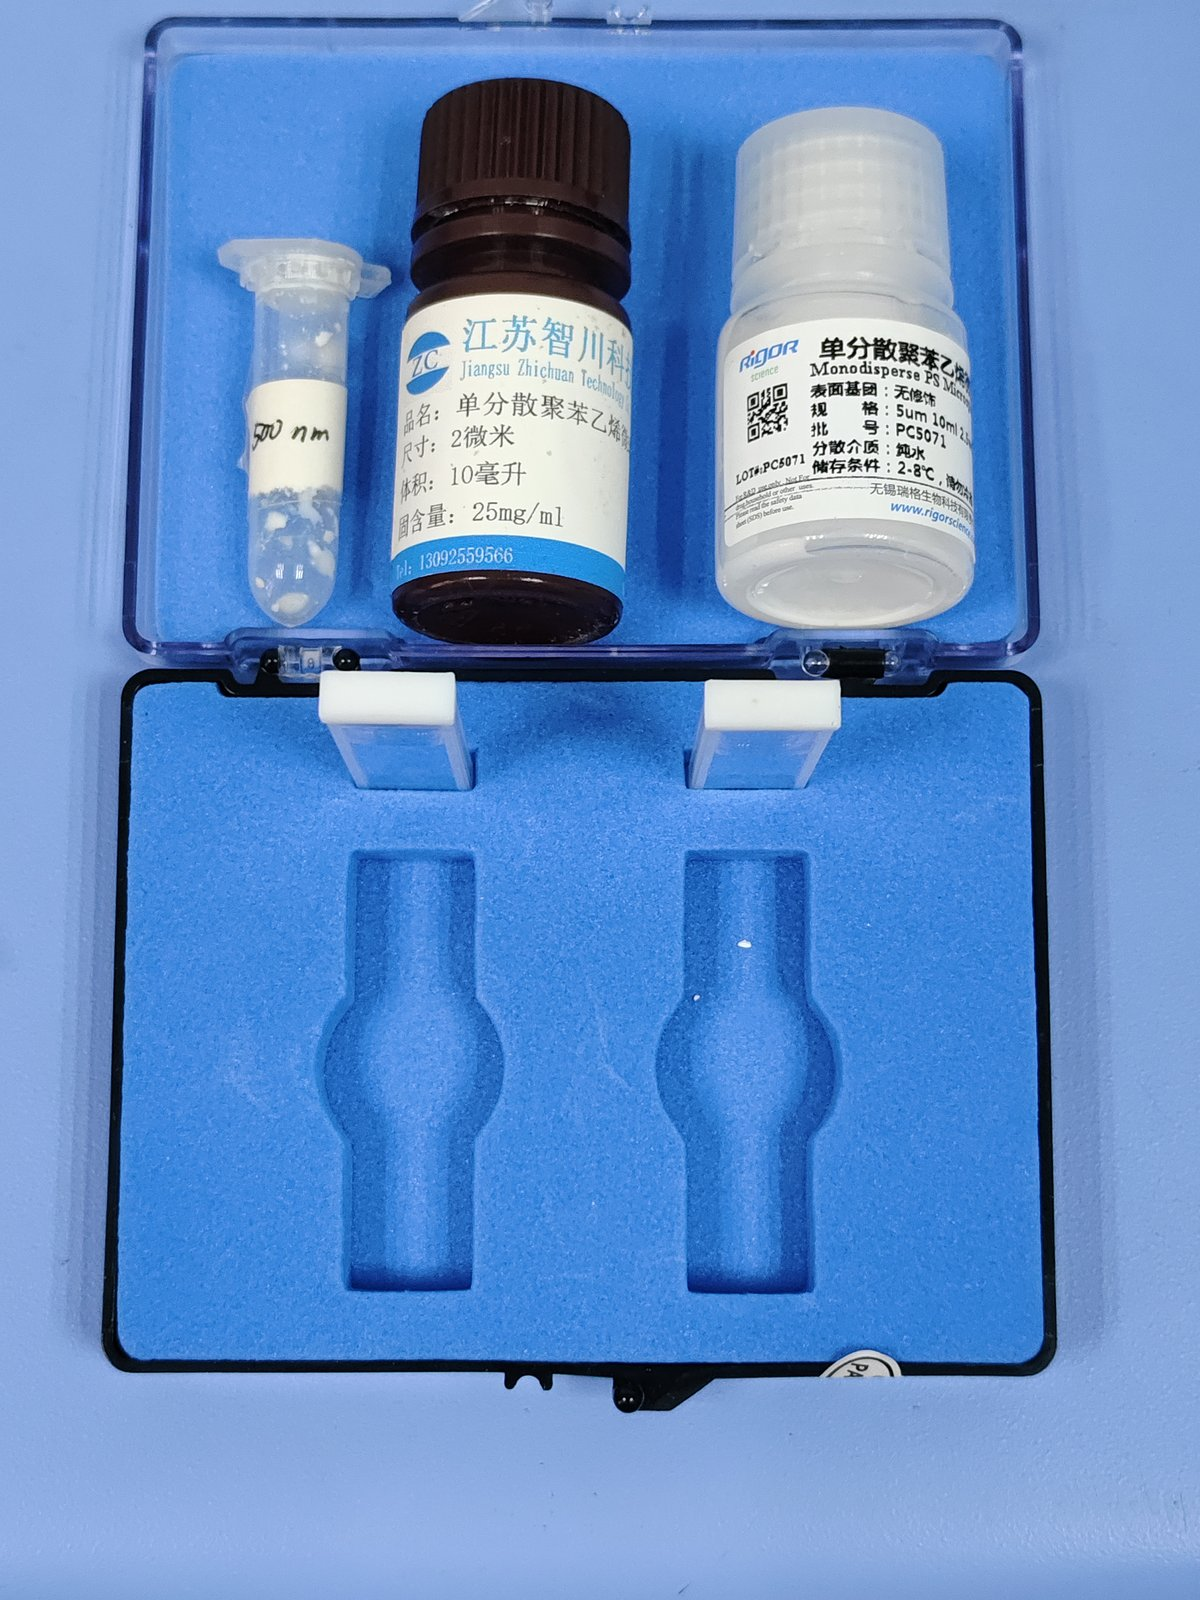
\includegraphics[width=\linewidth]{比色皿.jpg}
        \caption{比色皿与样品}
    \end{subfigure}
    \begin{subfigure}{0.22\textwidth}
        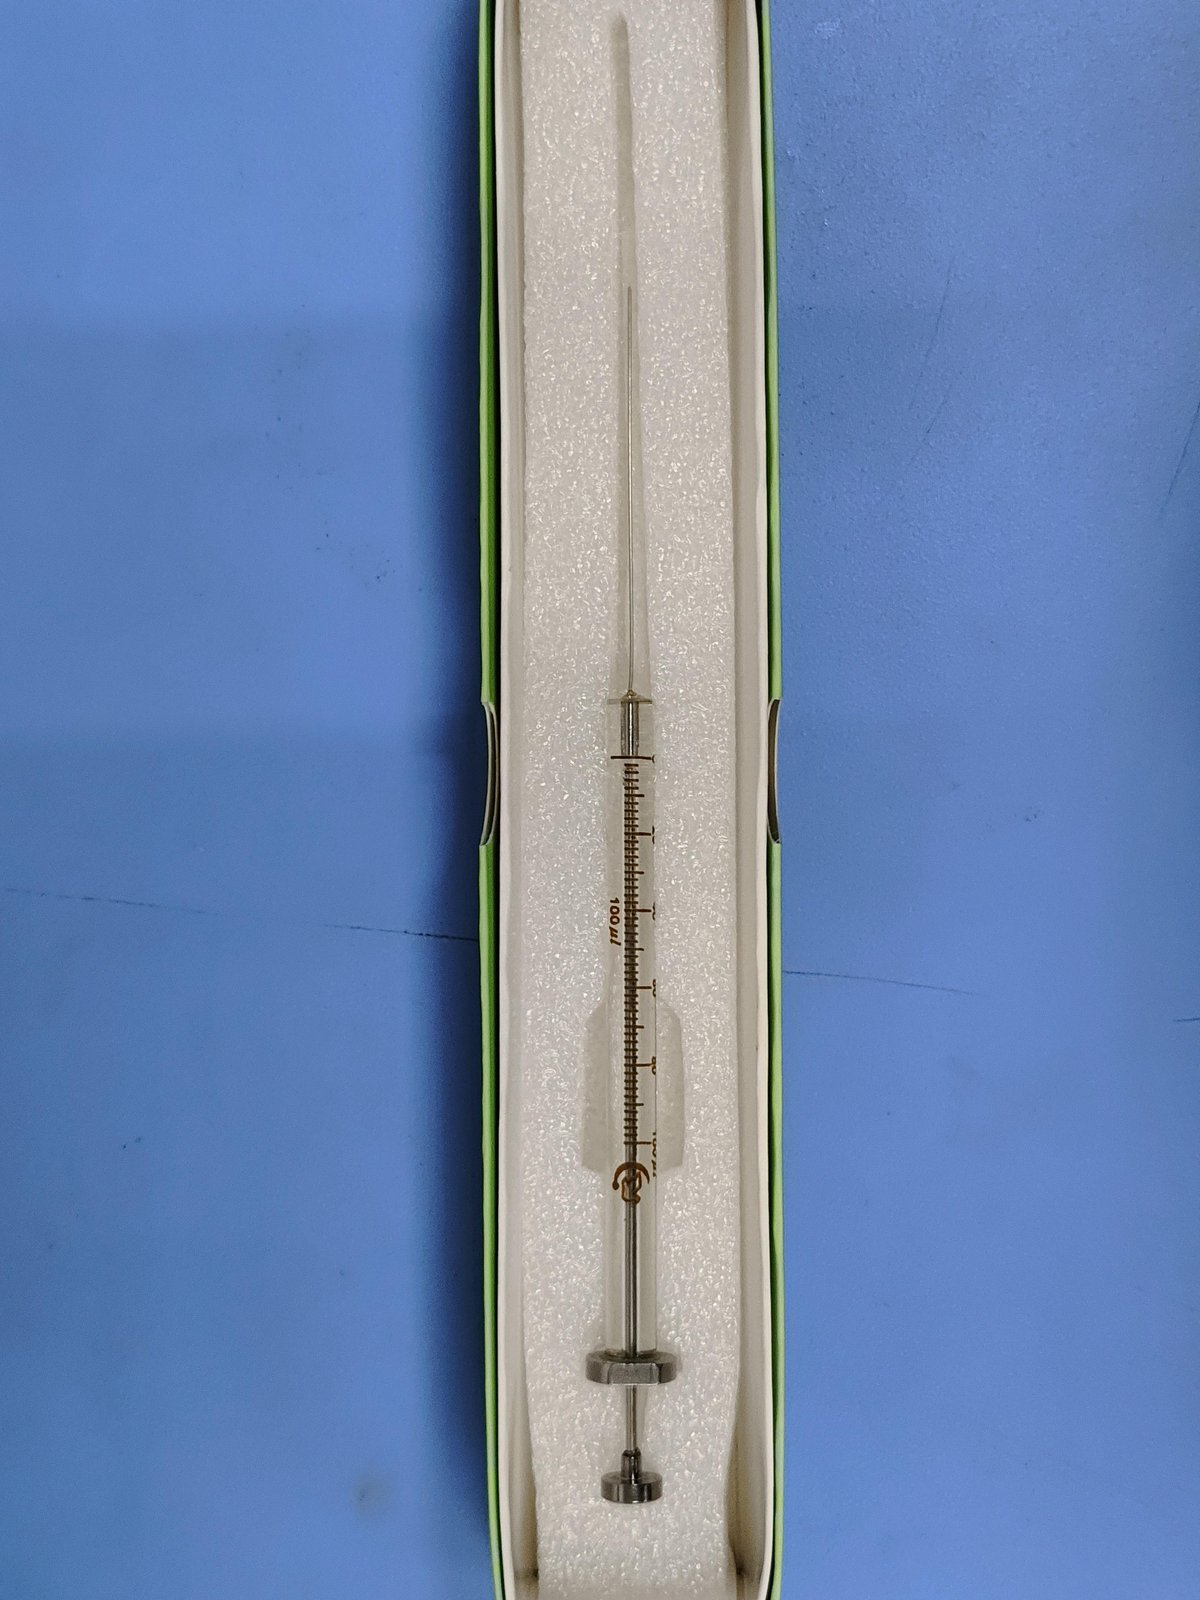
\includegraphics[width=\linewidth]{微量进样器.jpg}
        \caption{微量进样器}
    \end{subfigure}

    % 第二行
    \begin{subfigure}{0.22\textwidth}
        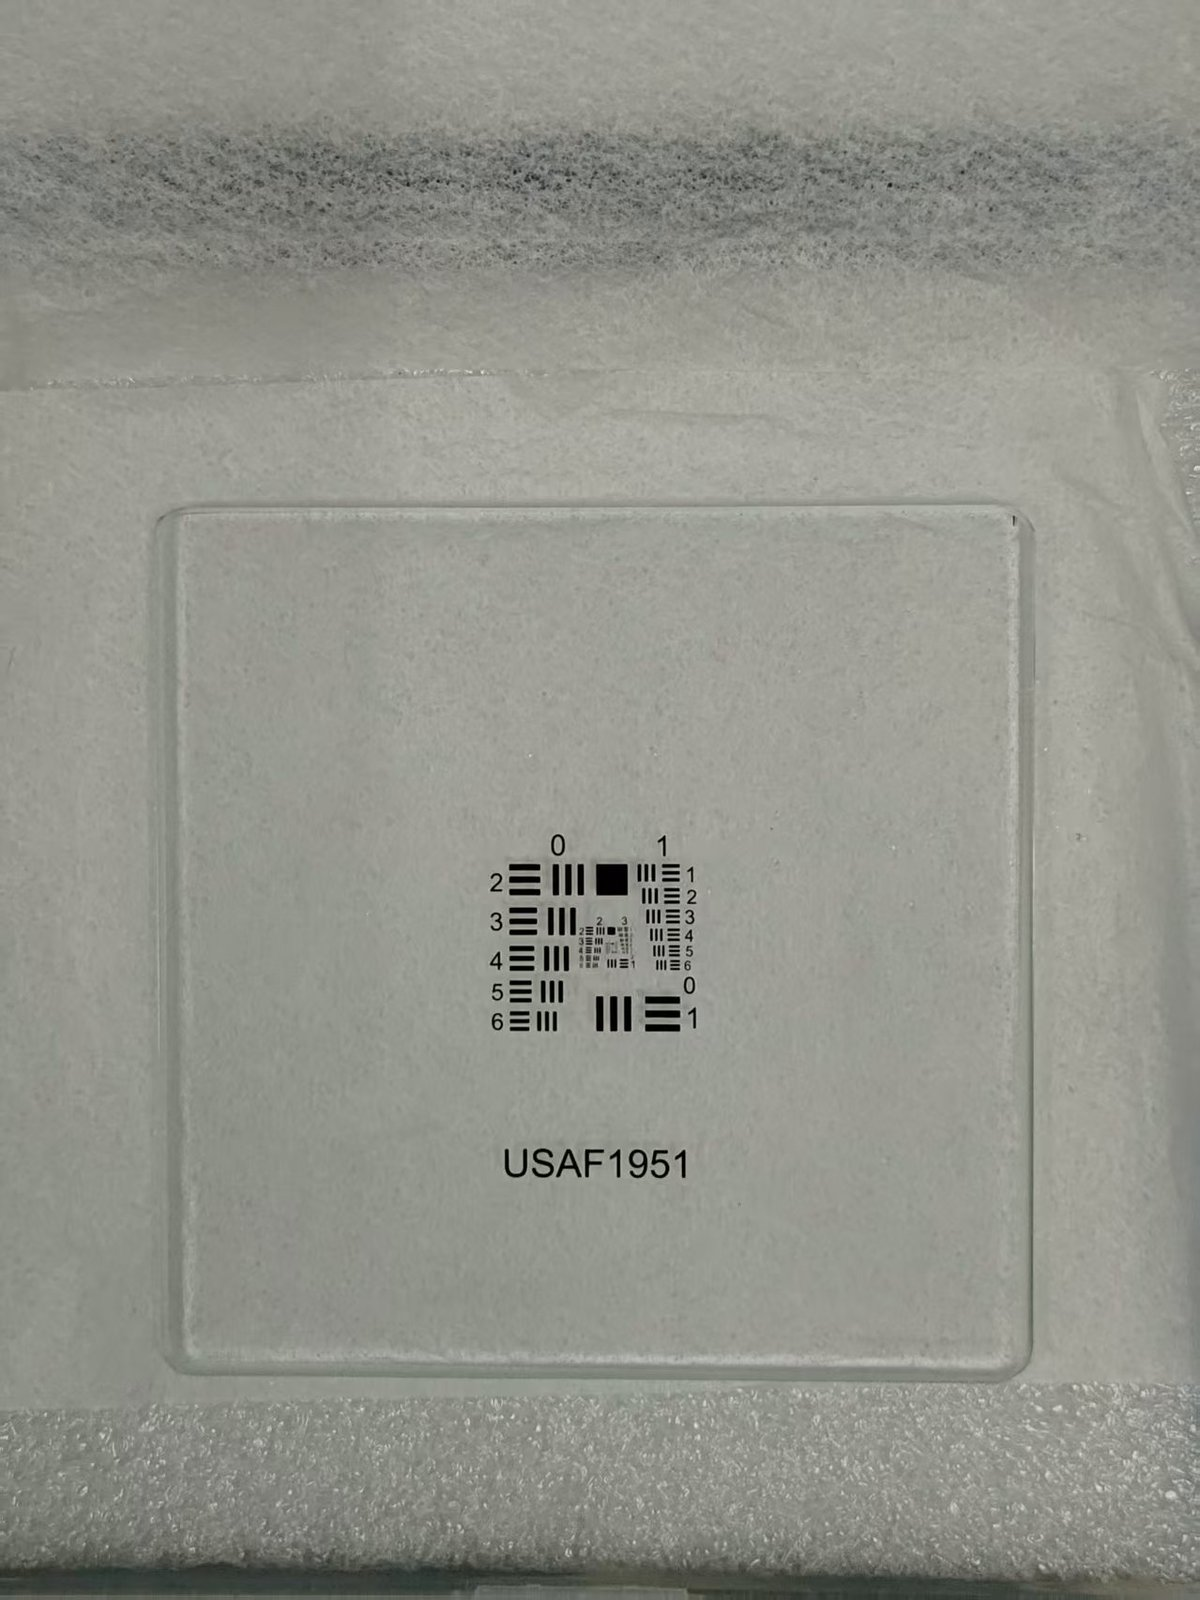
\includegraphics[width=\linewidth]{分辨率板.jpg}
        \caption{分辨率板}
    \end{subfigure}
    \begin{subfigure}{0.22\textwidth}
        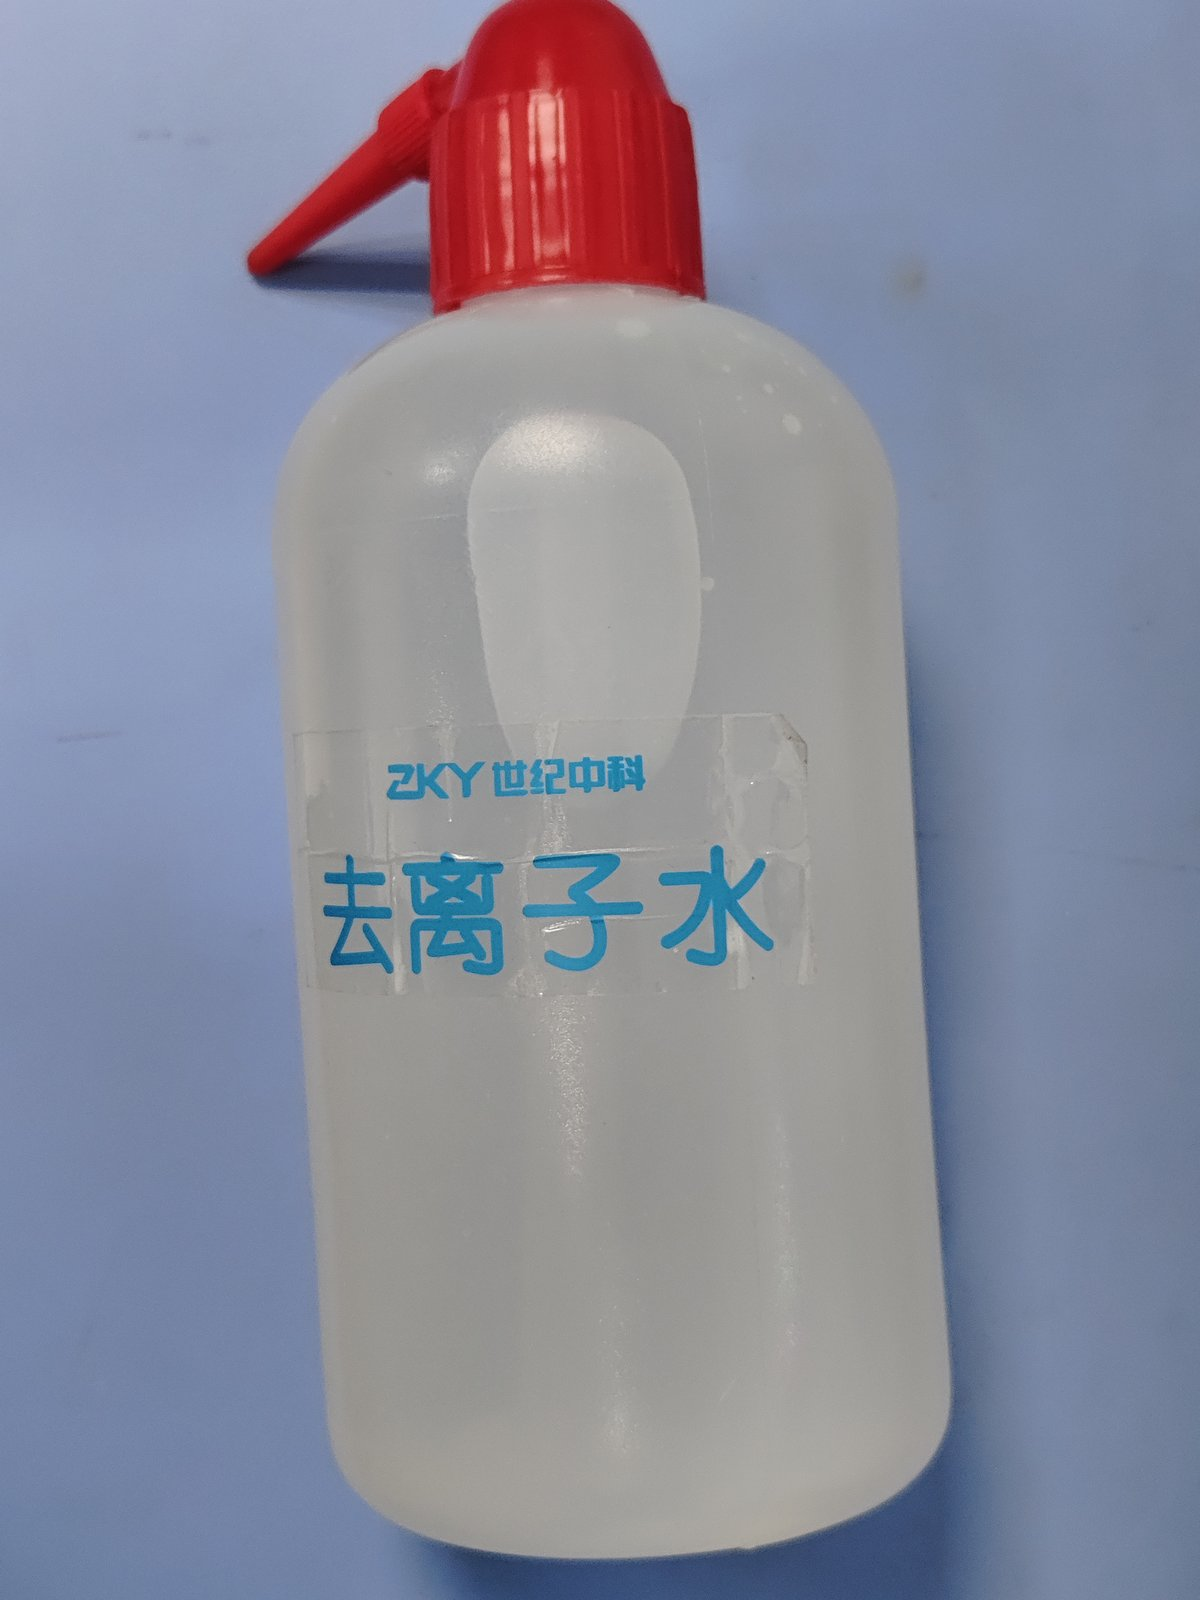
\includegraphics[width=\linewidth]{去离子水.jpg}
        \caption{去离子水}
    \end{subfigure}
    \begin{subfigure}{0.22\textwidth}
        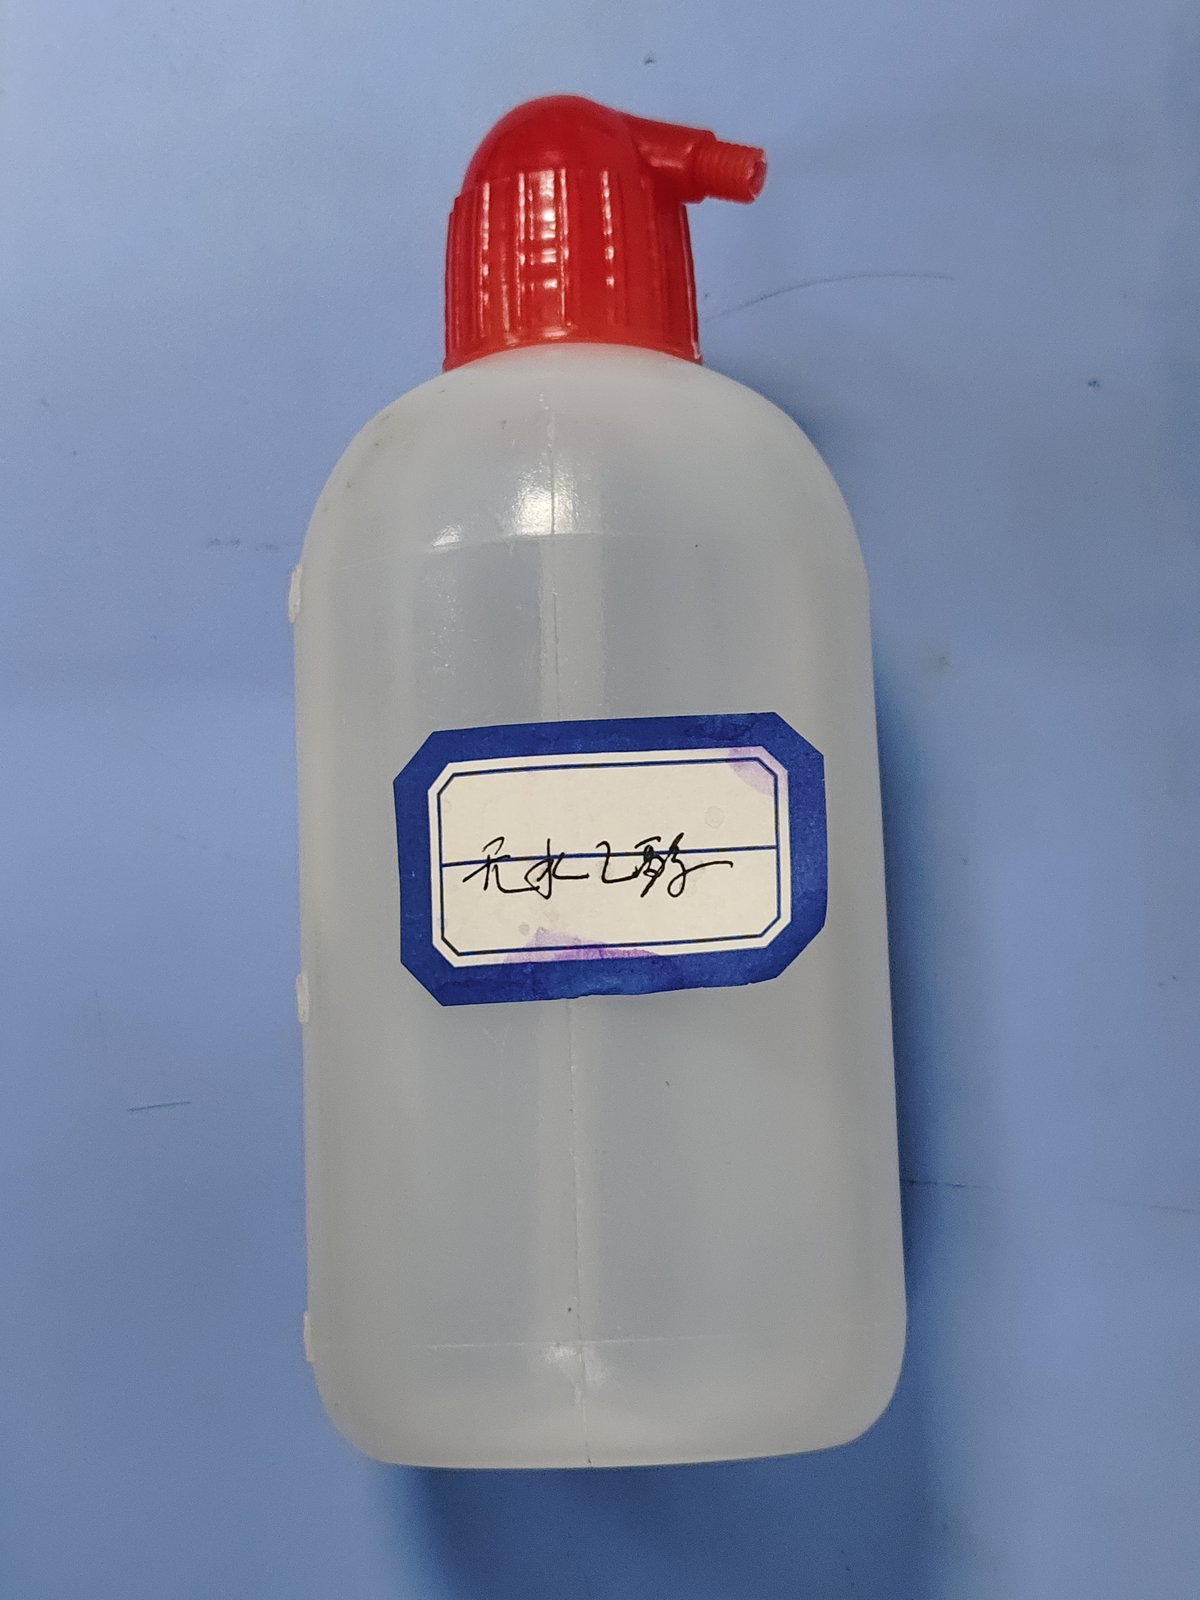
\includegraphics[width=\linewidth]{无水乙醇.jpg}
        \caption{无水乙醇}
    \end{subfigure}
    \begin{subfigure}{0.22\textwidth}
        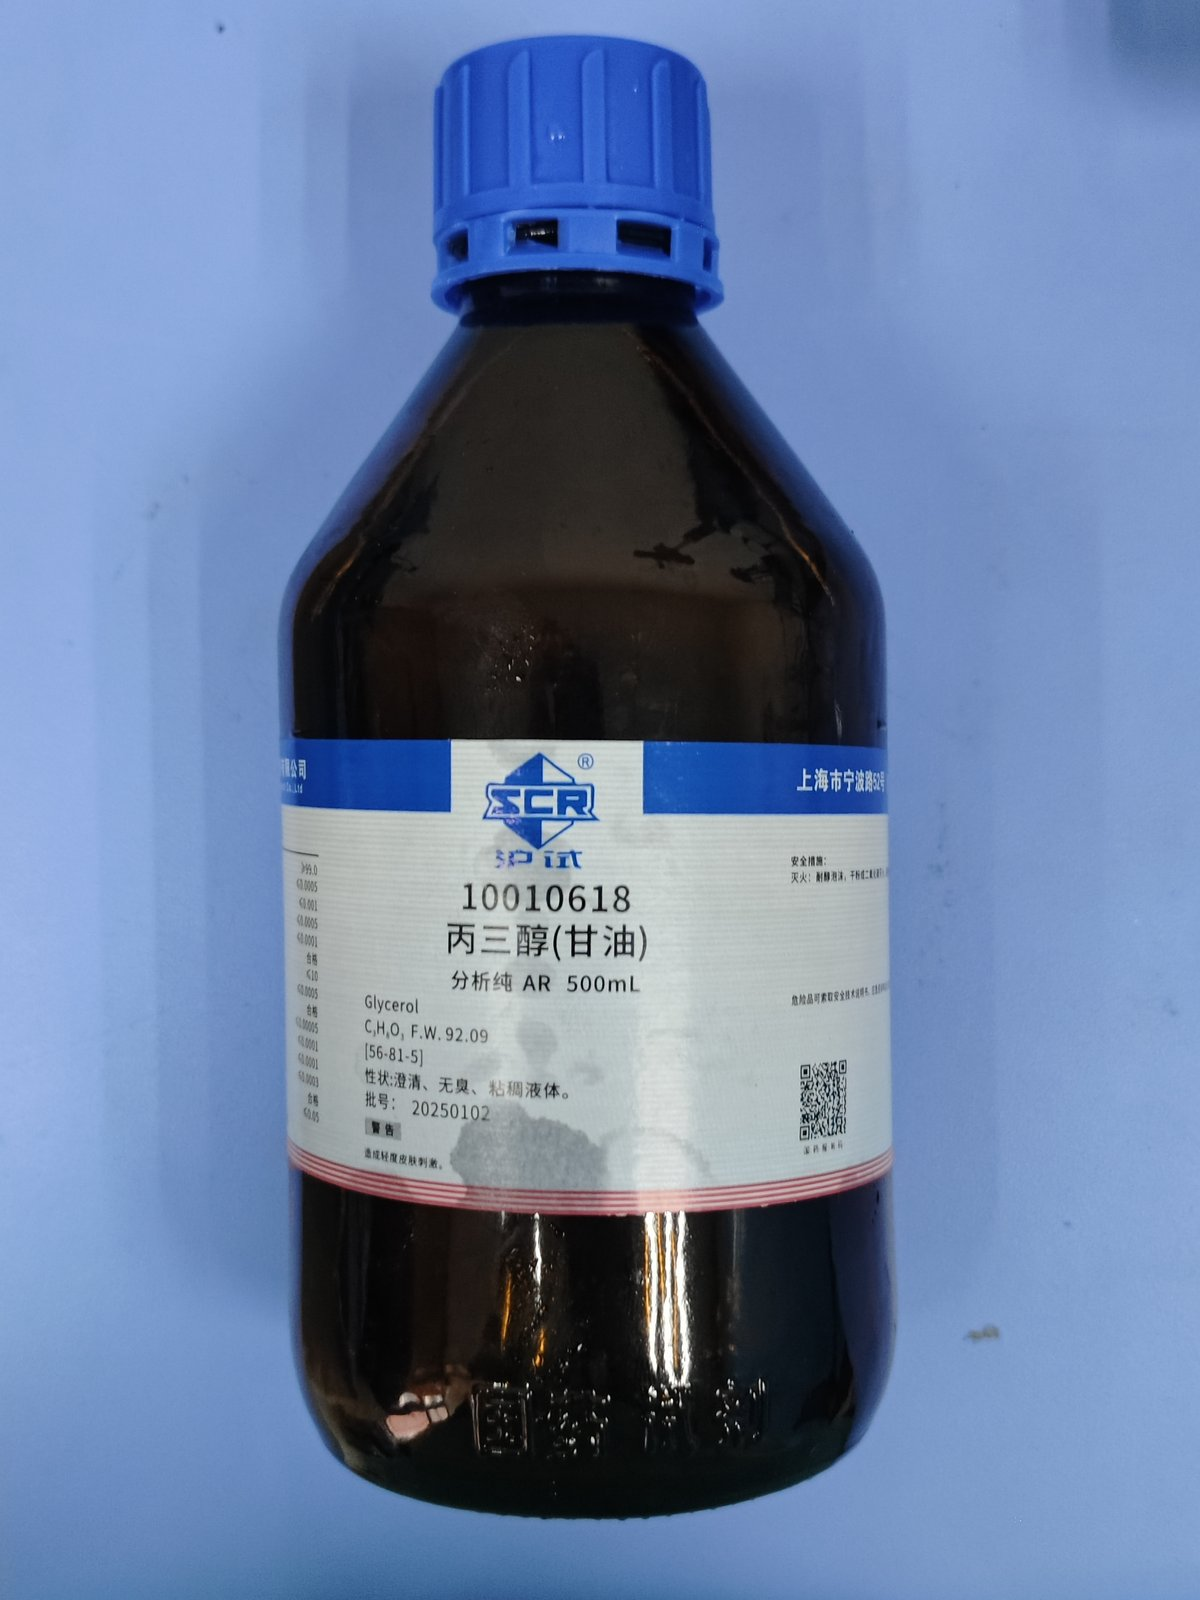
\includegraphics[width=\linewidth]{甘油.jpg}
        \caption{甘油}
    \end{subfigure}

    % 第三行
    \begin{subfigure}{0.22\textwidth}
        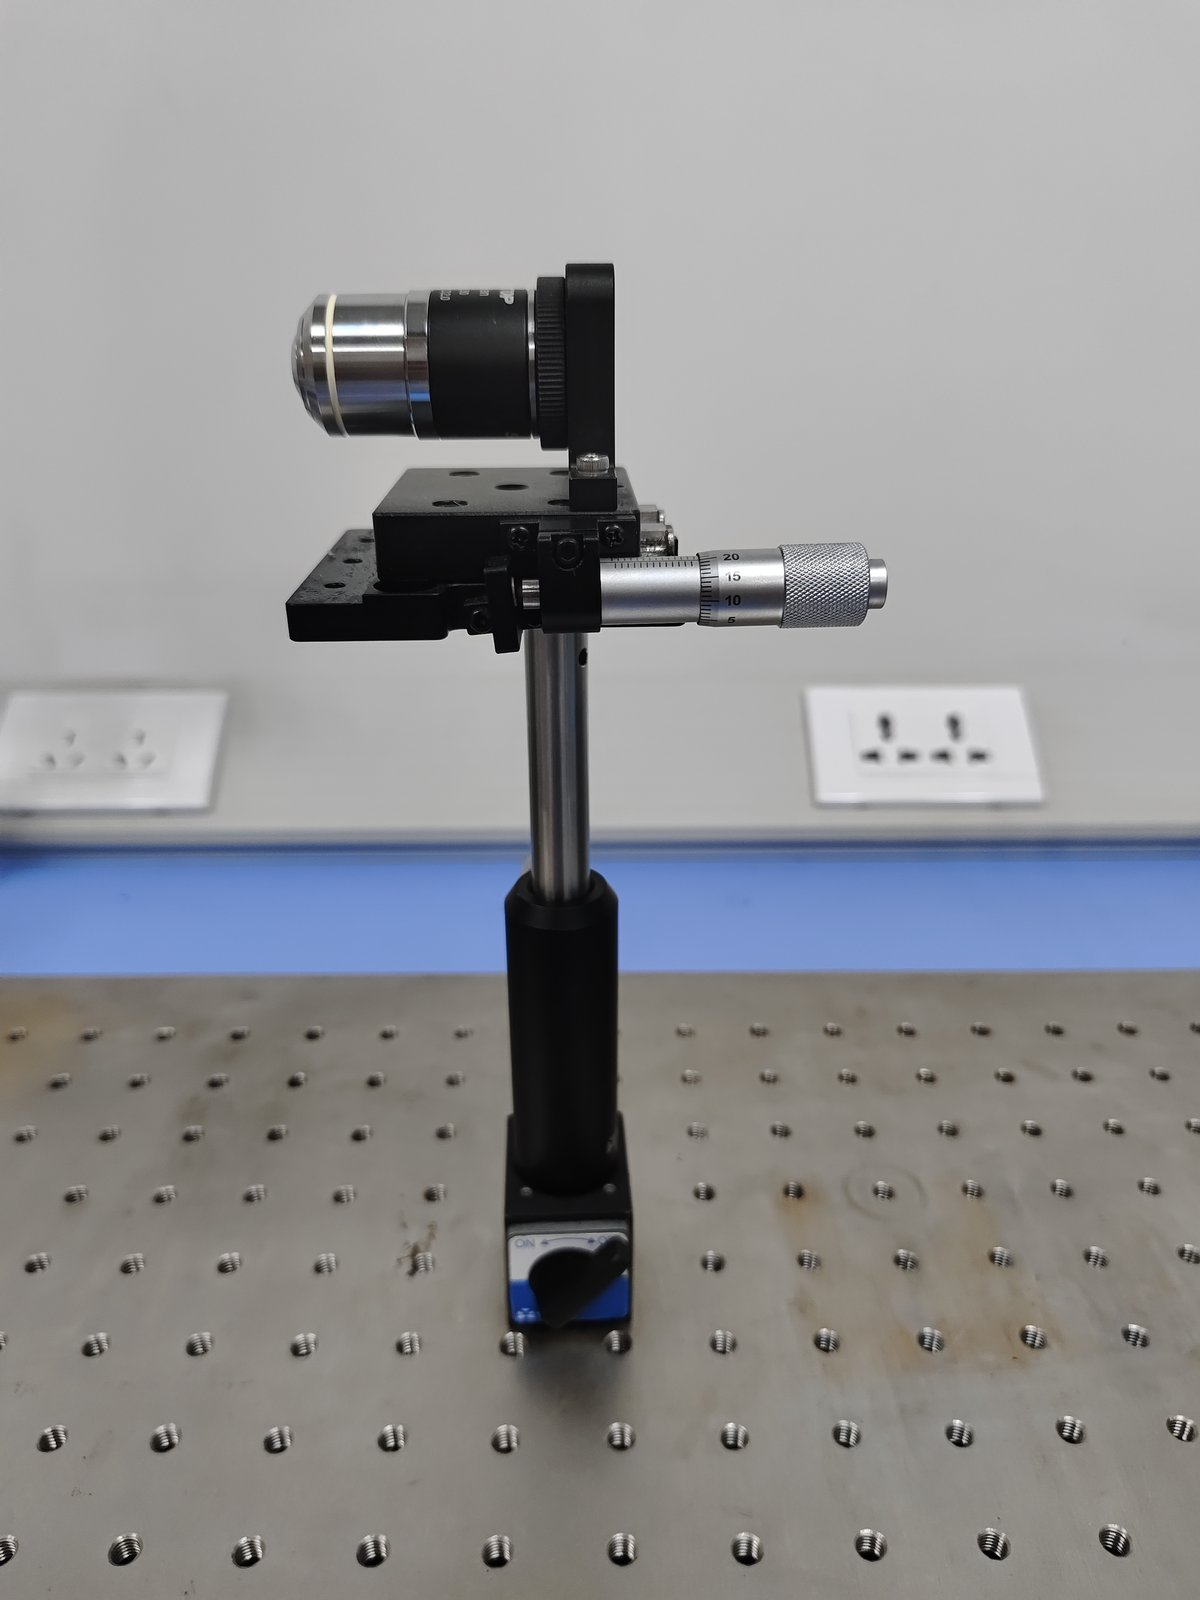
\includegraphics[width=\linewidth]{100x物镜.jpg}
        \caption{100x物镜}
    \end{subfigure}
    \begin{subfigure}{0.22\textwidth}
        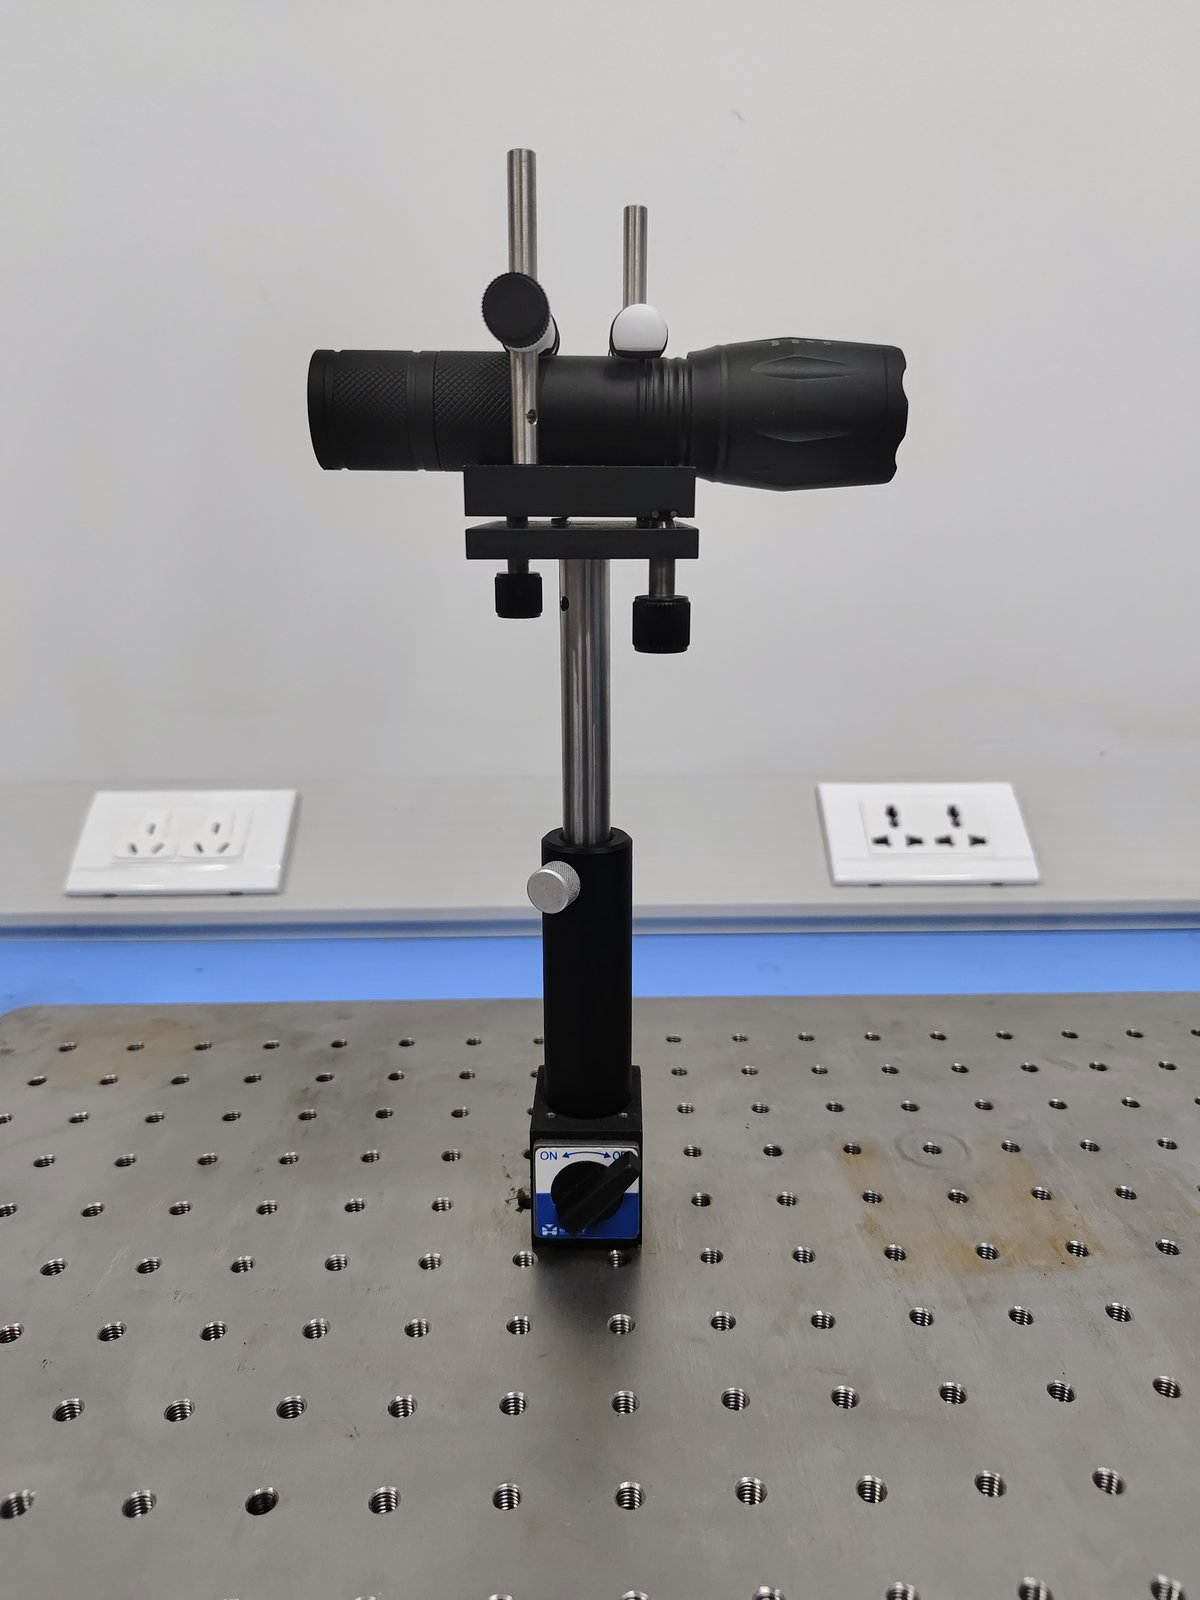
\includegraphics[width=\linewidth]{非相干光源.jpg}
        \caption{非相干光源}
    \end{subfigure}
    \begin{subfigure}{0.22\textwidth}
        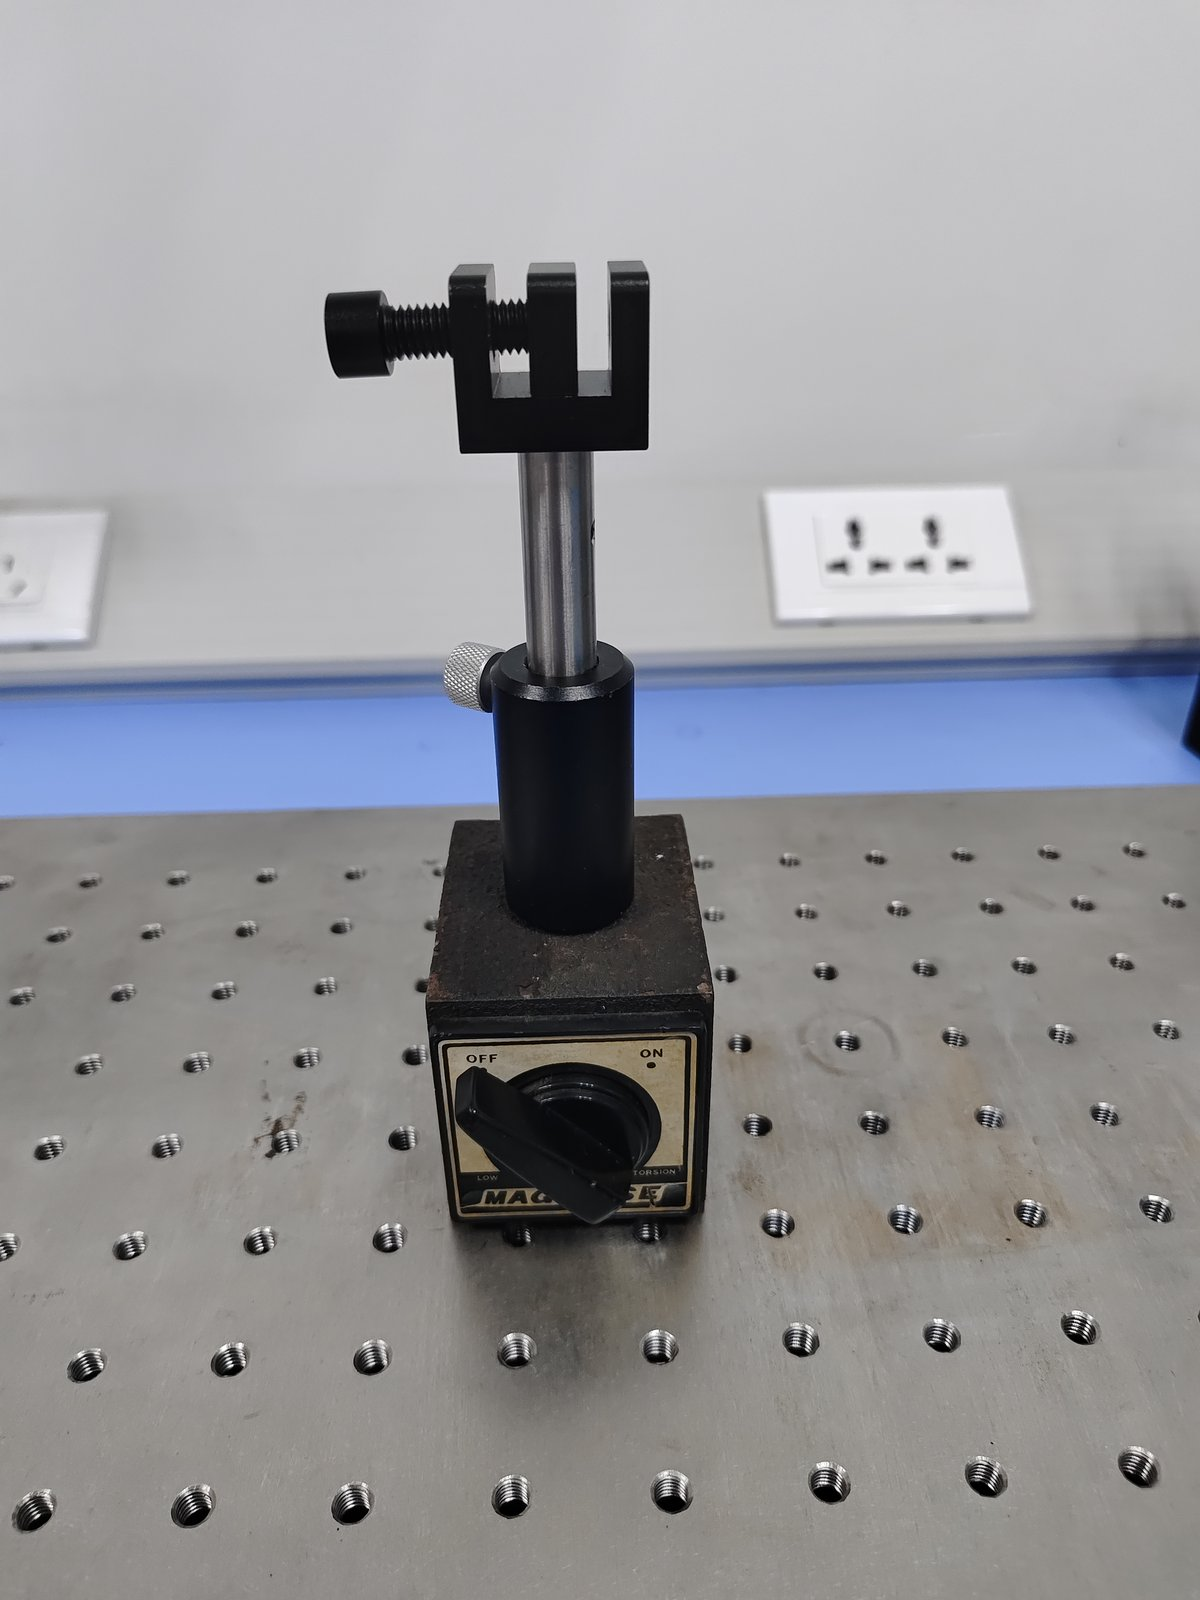
\includegraphics[width=\linewidth]{夹具1.jpg}
        \caption{夹具}
    \end{subfigure}
    \begin{subfigure}{0.22\textwidth}
        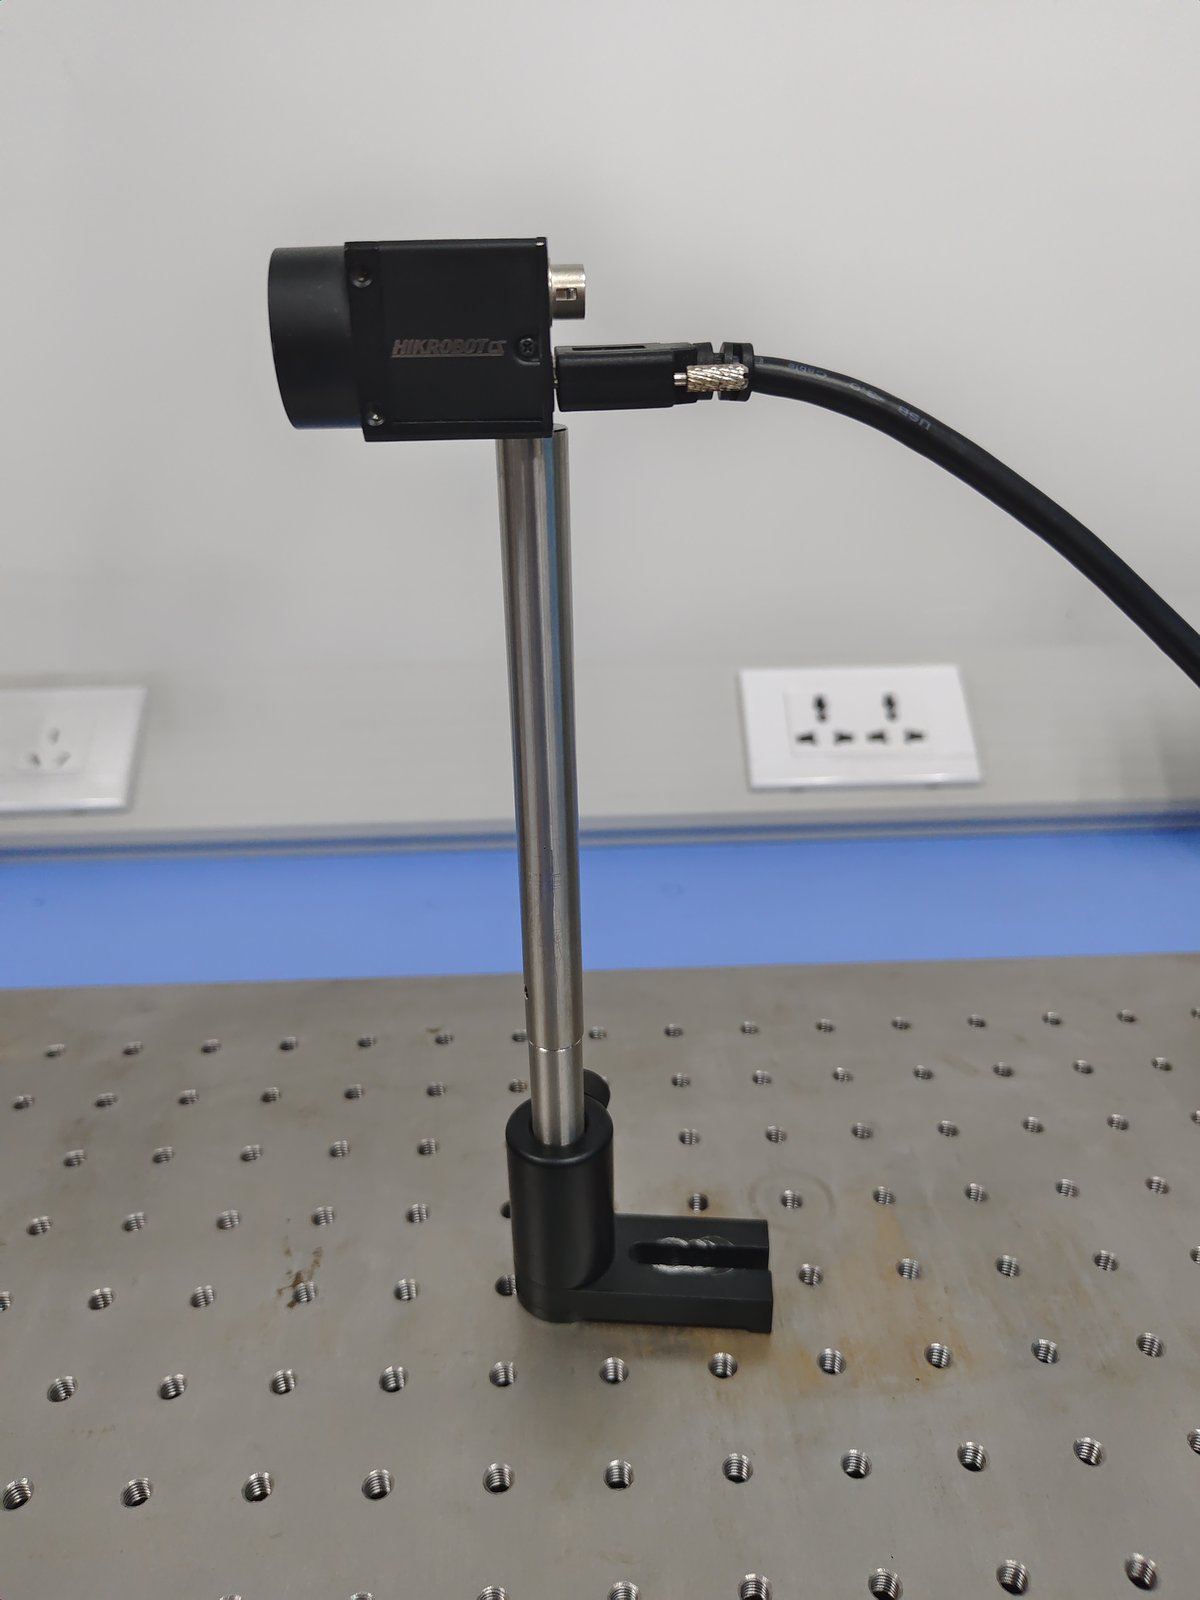
\includegraphics[width=\linewidth]{CCD.jpg}
        \caption{CCD}
    \end{subfigure}

    % 第四行
    \begin{subfigure}{0.22\textwidth}
        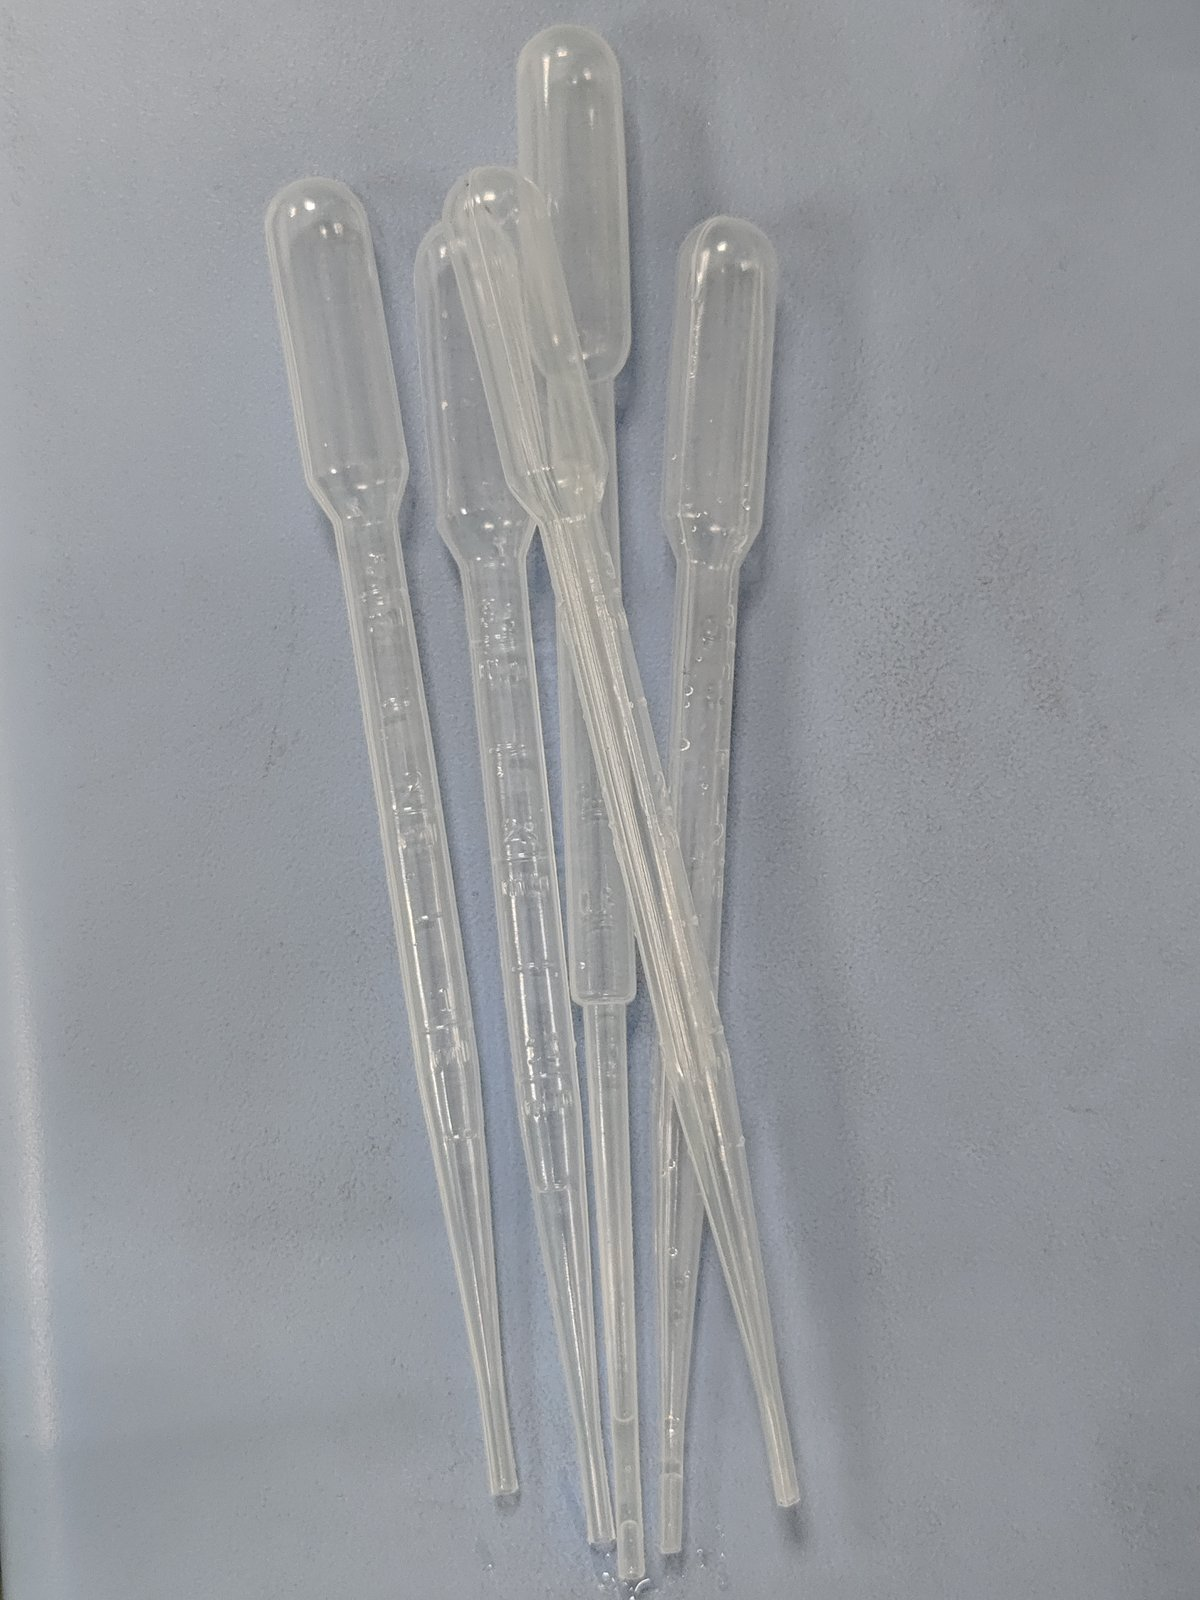
\includegraphics[width=\linewidth]{胶头滴管.jpg}
        \caption{胶头滴管}
    \end{subfigure}
    \begin{subfigure}{0.22\textwidth}
        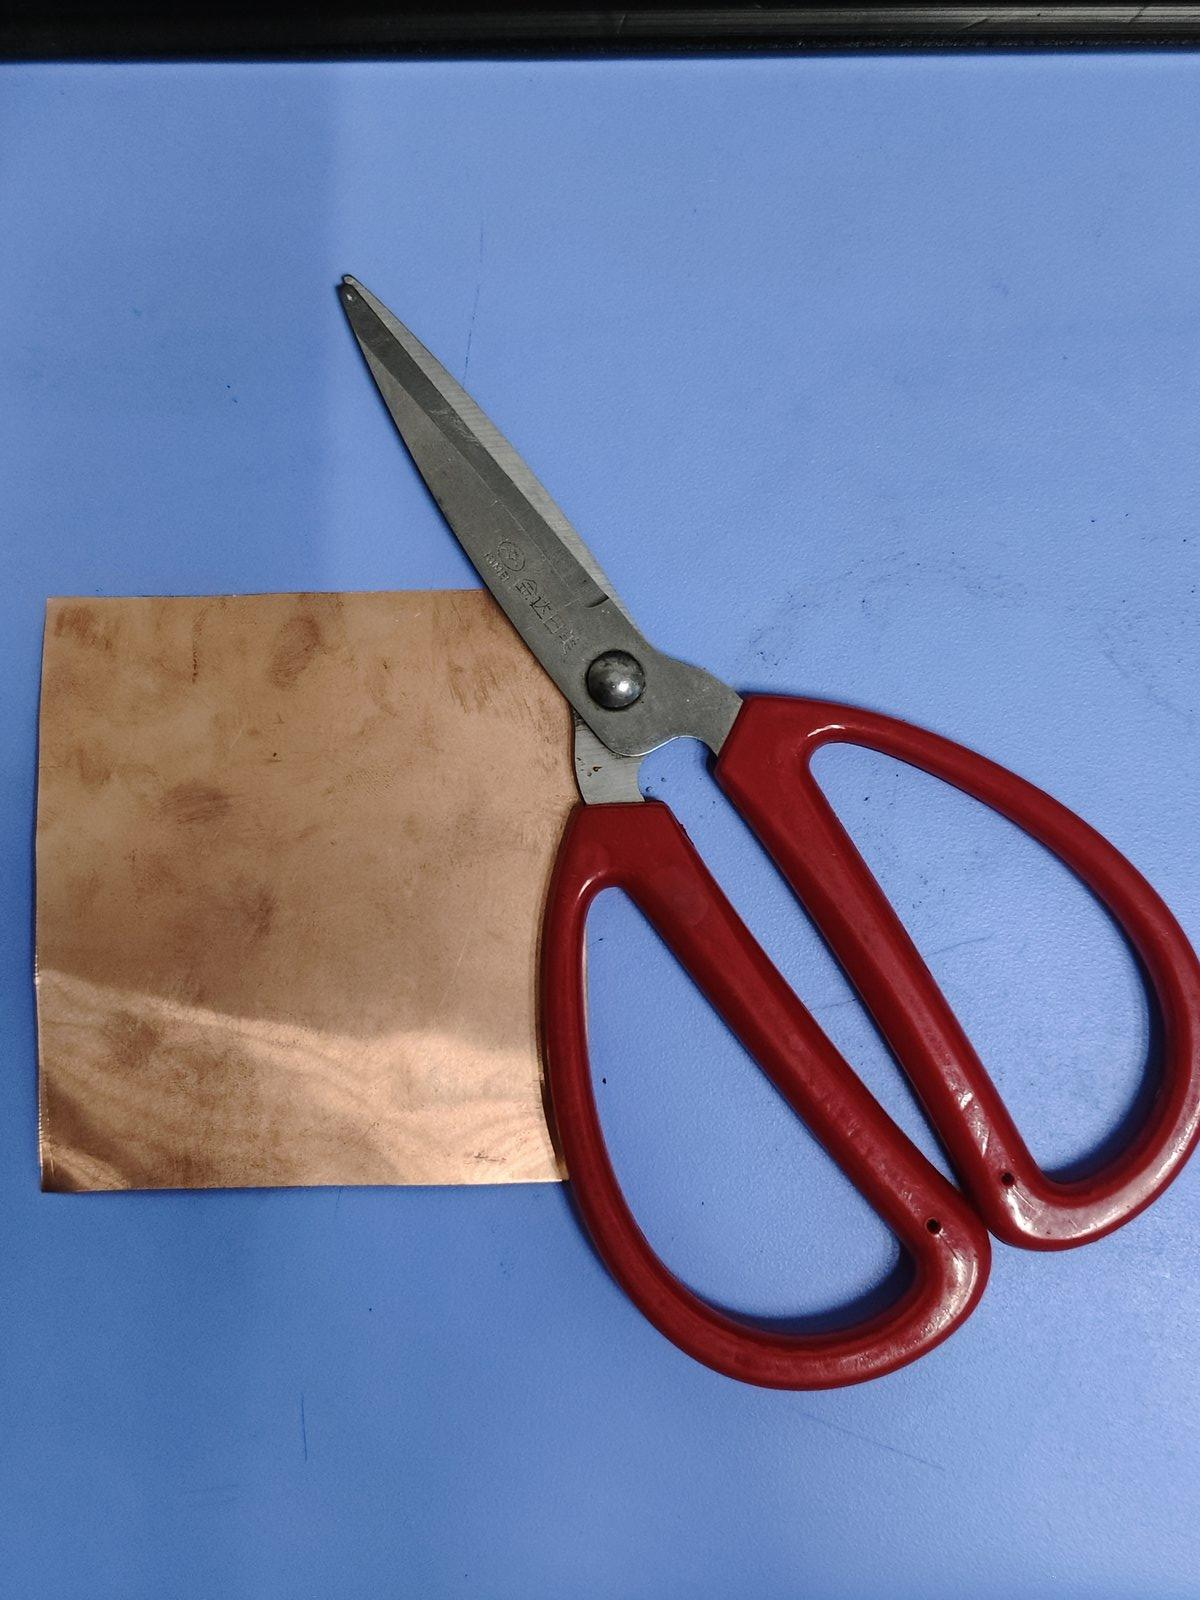
\includegraphics[width=\linewidth]{剪刀与铜片.jpg}
        \caption{剪刀与铜片}
    \end{subfigure}
    \begin{subfigure}{0.22\textwidth}
        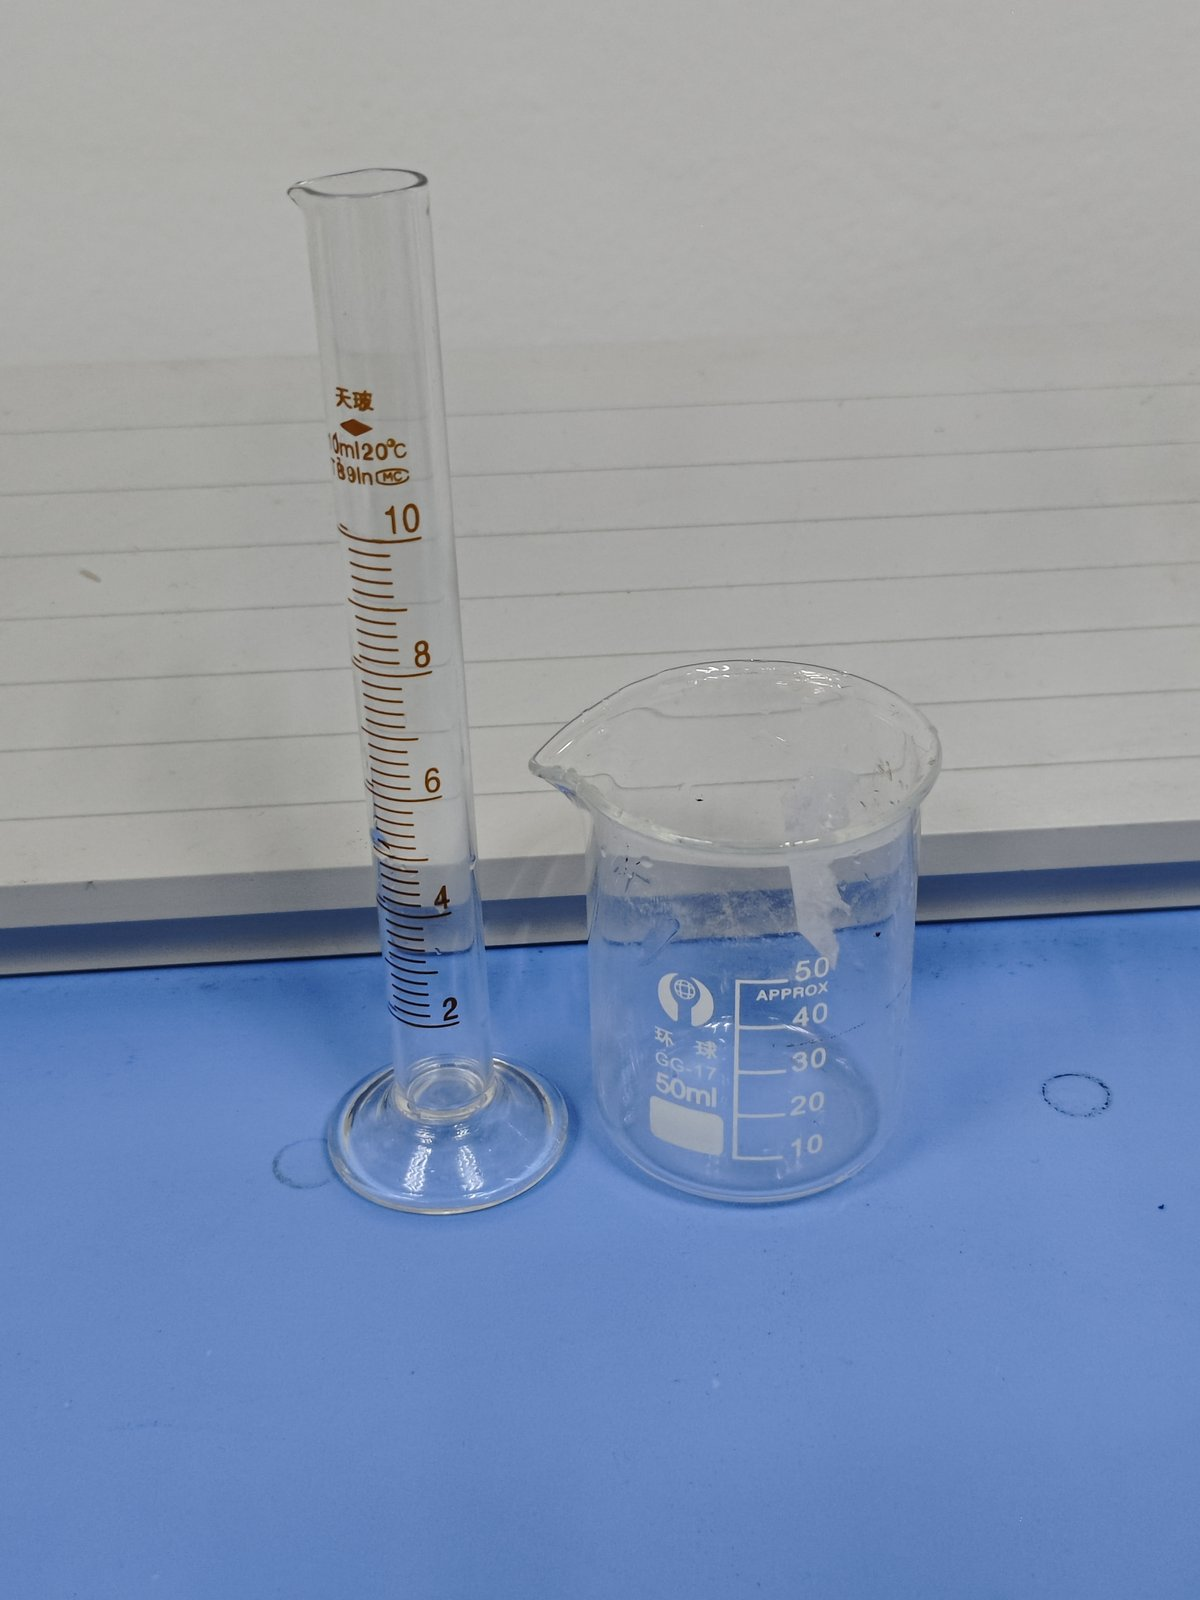
\includegraphics[width=\linewidth]{烧杯与量筒.jpg}
        \caption{烧杯与量筒}
    \end{subfigure}
    \begin{subfigure}{0.22\textwidth}
        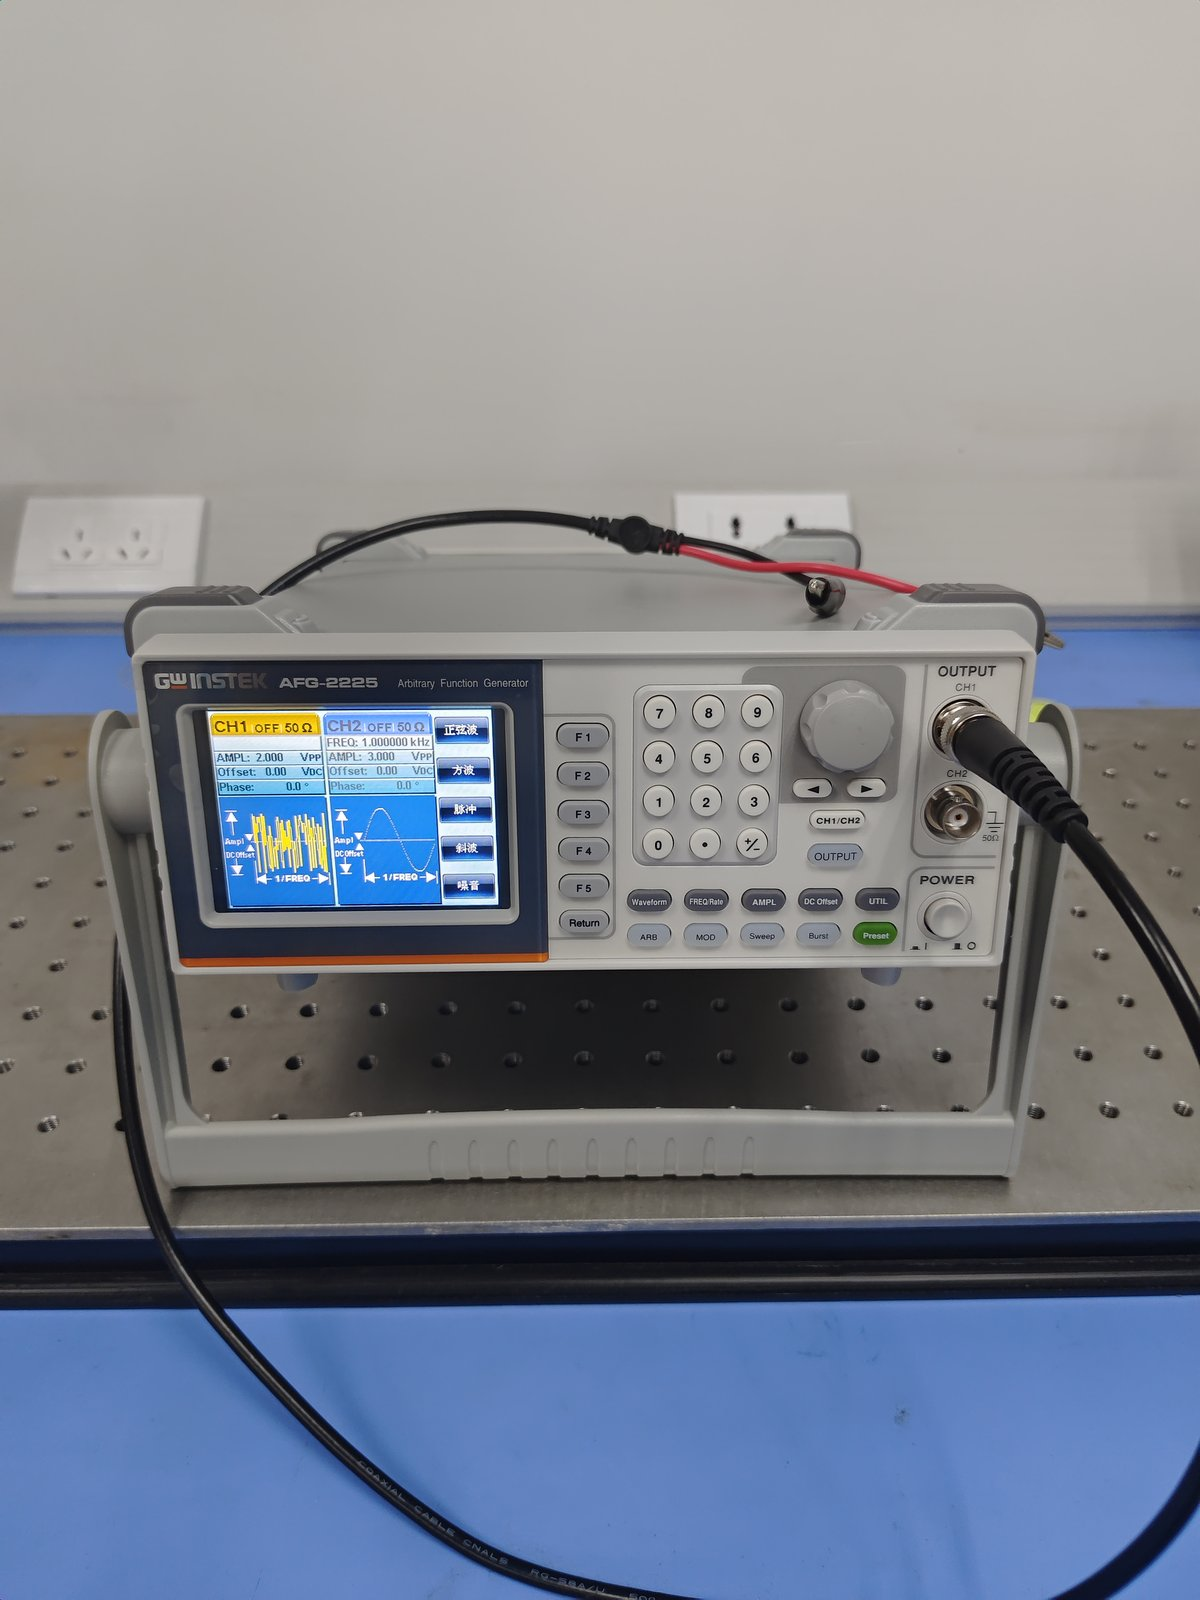
\includegraphics[width=\linewidth]{信号发生器.jpg}
        \caption{信号发生器}
    \end{subfigure}

    \caption{实验仪器}
\end{figure}

\section{实验装置与示意图}

\begin{figure}[H]
    \centering
    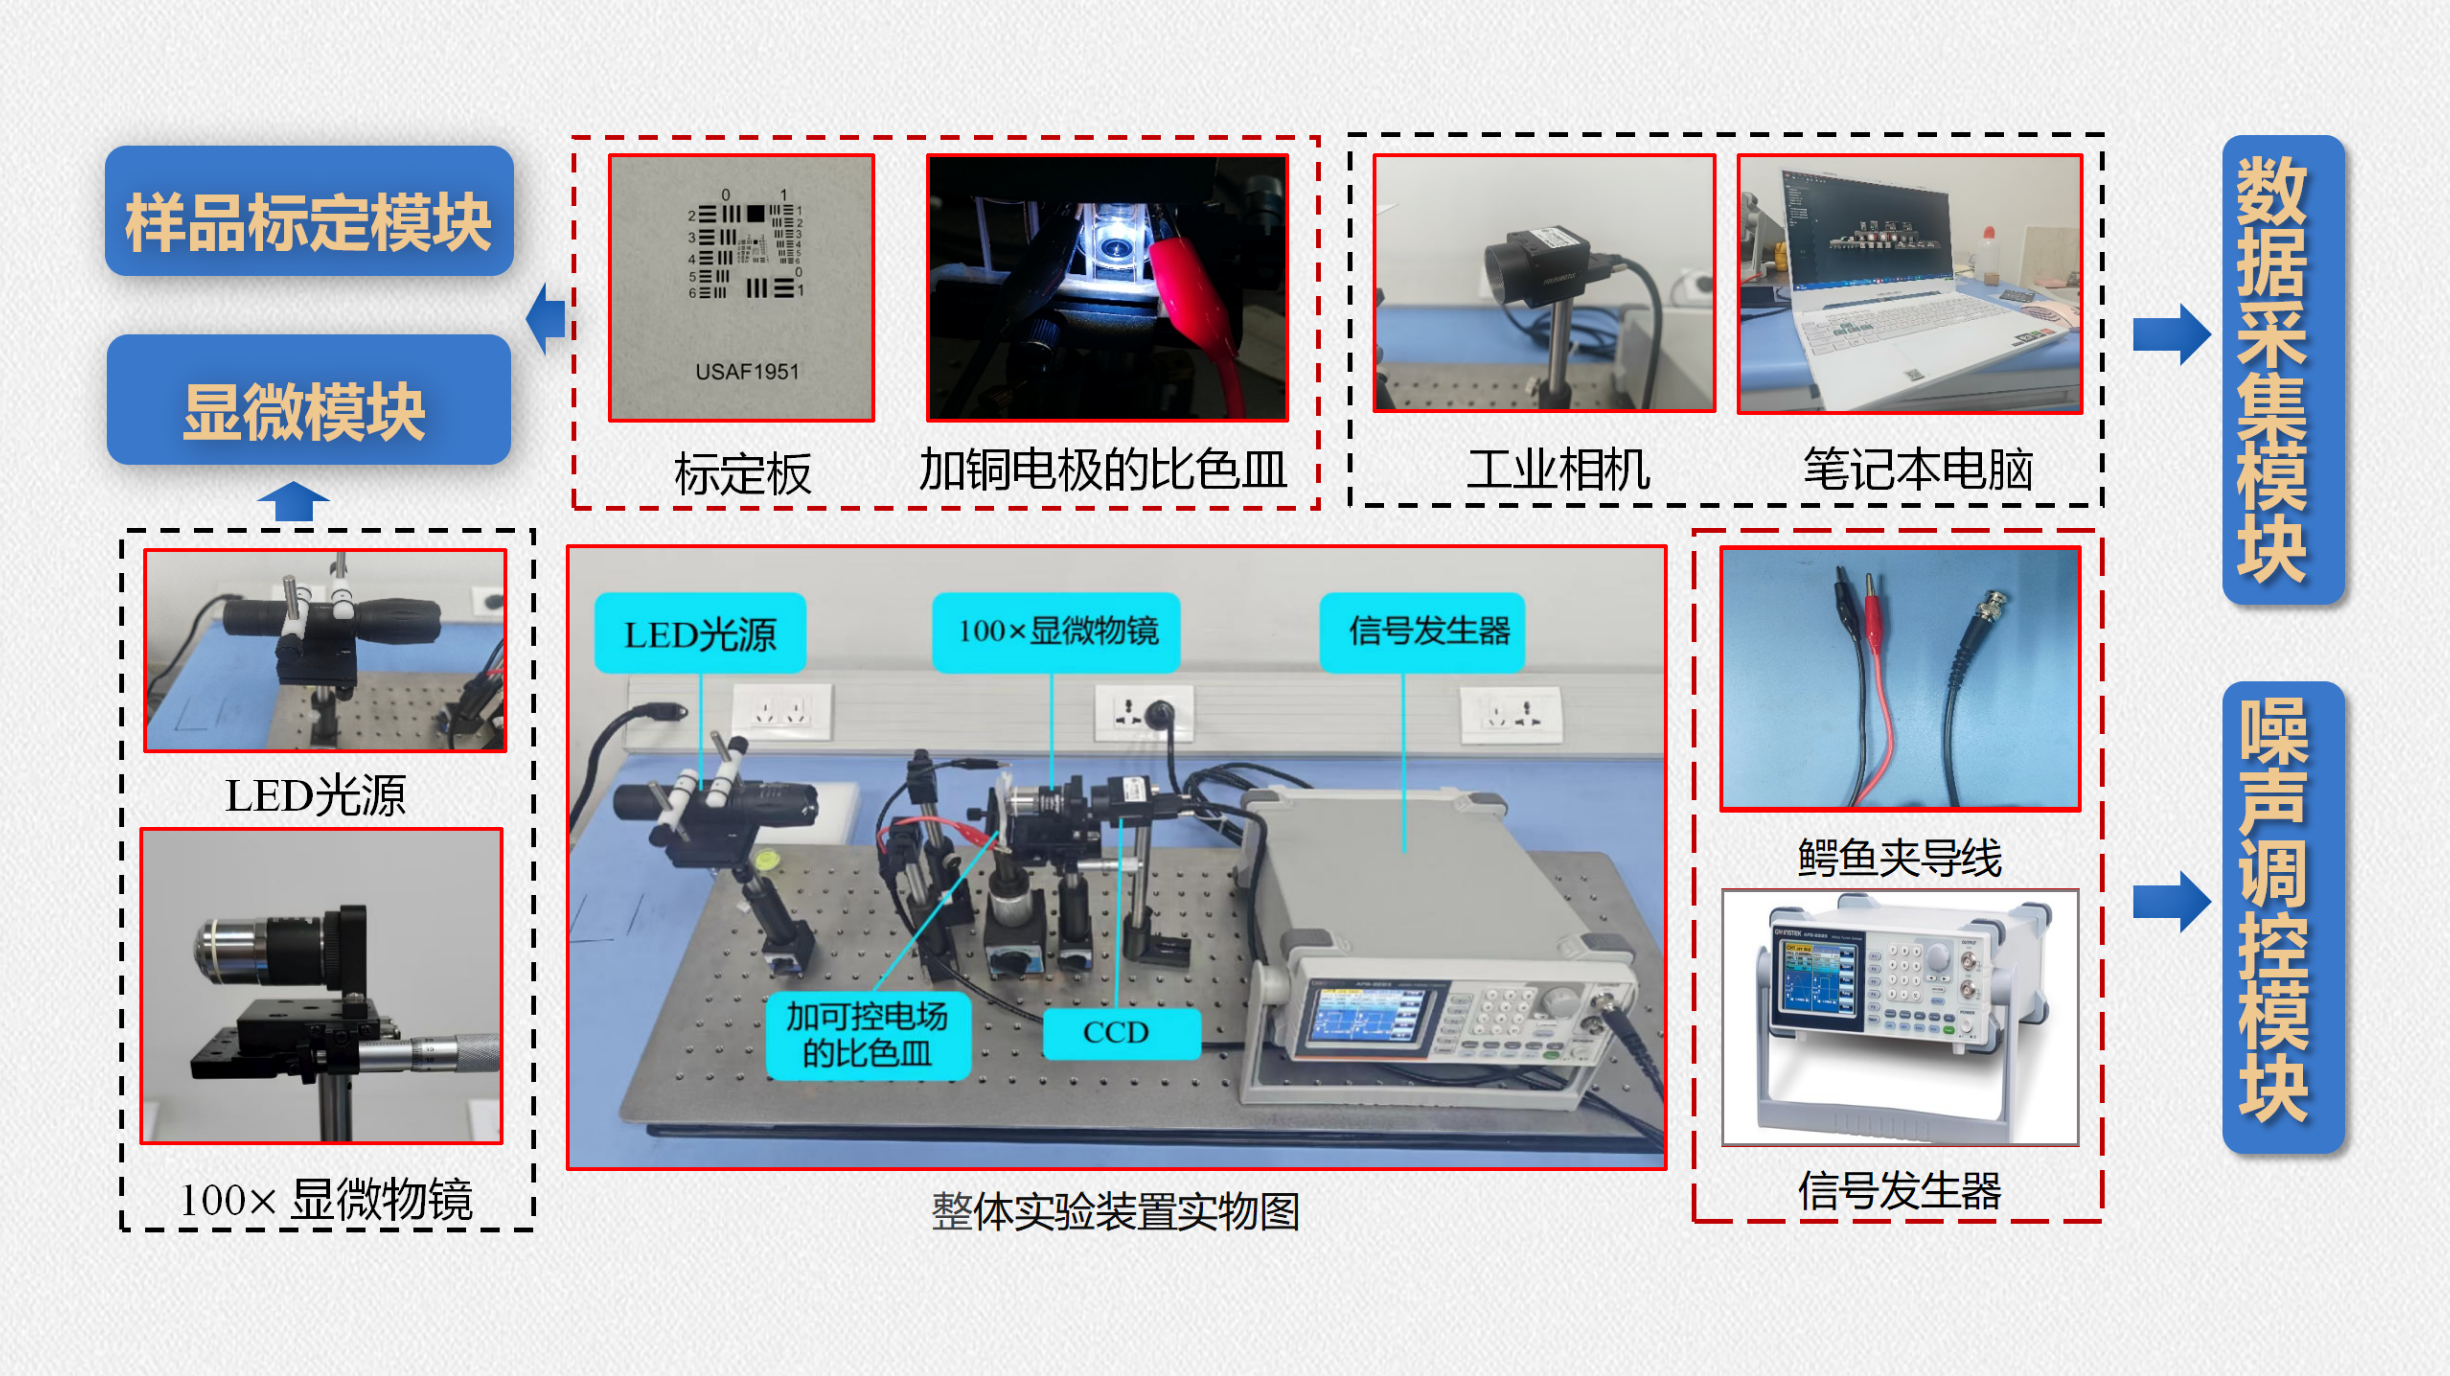
\includegraphics[width=1.0\textwidth]{实验装置模块.png}
    \caption{实验装置与模块}
    \label{fig:allsetup}
\end{figure}
\begin{figure}[H]
    \centering
    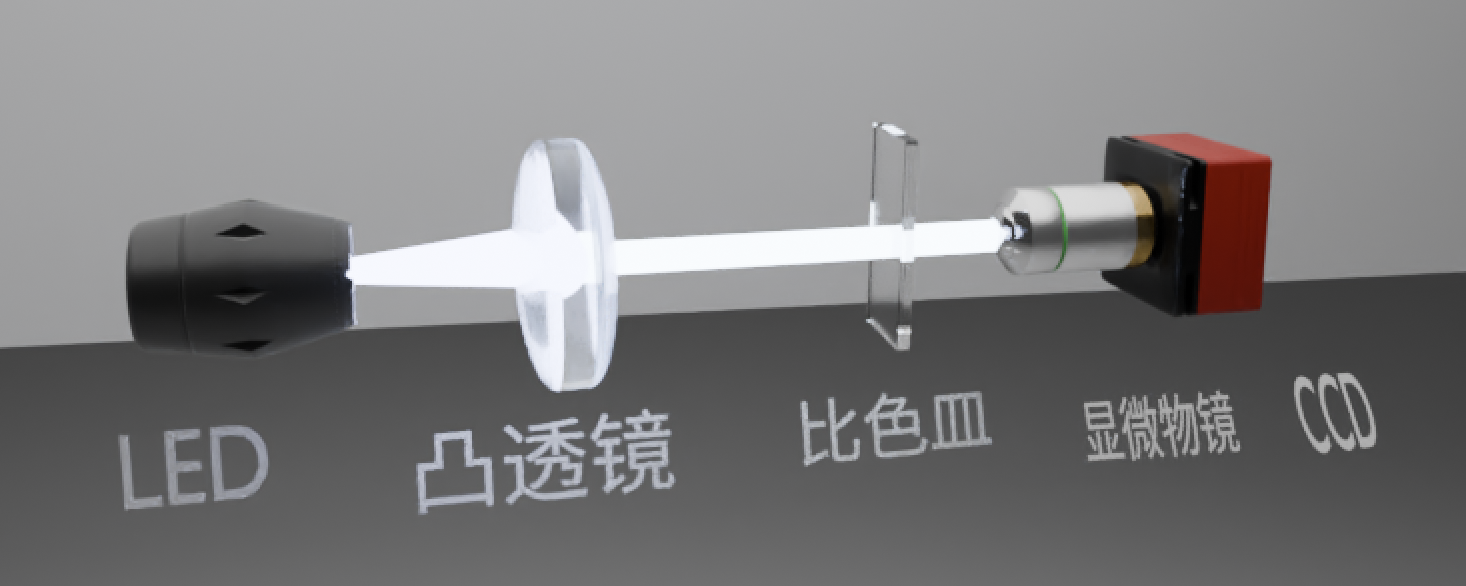
\includegraphics[width=0.9\textwidth]{实验示意图.png}
    \caption{实验装置示意图}
    \label{fig:sets}
\end{figure} 
\section{仪器性能指标评定}

\section{局限性与误差来源分析}
(1)在进行分辨率板的标定实验中,虽然我们确定了当分辨率板位于物镜工作平面时,相机每个像素对应的距离,但是在将分辨率板换为比色皿时,
由于比色皿的厚度与分辨率板的厚度并不相同,且无法保证视野内观察到比色皿中的微球。此时,需要前后稍微移动物镜来使视野内有我们想要观察的PS微球。 \par
(2)配制甘油与水的混合比例时,取一定量的水和甘油时会引入误差。\par
(3)微球的浓度分布也会造成误差:微球浓度过高可能导致重叠或遮挡,浓度过低则统计样本不足;溶液未充分混合或存在团聚会影响扩散行为的代表性。\par
(4)由于电极的宽度只有2mm,因此电极加载的电场会由于边缘效应而不均匀,电极未完全平行或紧贴比色皿壁,导致电场分布不均匀,影响等效温度实验的电压控制效果。\par
(5)采集的粒子数量和时间有限,统计平均值可能与真实值有偏差。我们计算的物理量是基于统计平均的,因此对于有限的数据量,会由于随机性等产生误差。\par
(6)不同的粒子识别算法与追踪算法也会带来误差,而且在图像中,粒子边缘模糊或多个粒子重叠会导致识别错误。\par

\section{改进和优化思路}

\chapter{实验内容}

\section{实验操作}
\subsection{实验步骤}
1.按照图~\ref{fig:allsetup}搭建光路,其示意图如图~\ref{fig:sets}所示,开启 LED 光源,保证LED光经过聚光镜后均匀照射在比色皿(或分辨率板)上,
固定好LED,显微物镜,和CCD相机后,进行标定实验。
标定实验:首先将分辨率板放在夹具上,打开LED,将CCD放在物镜后适当位置,前后调整物镜以使分辨率板的图像变得清晰可见,如下图~\ref{fig:biaoding}
\begin{figure}[H]
    \centering
    % 每行 2 张
    \begin{subfigure}{0.45\textwidth}
        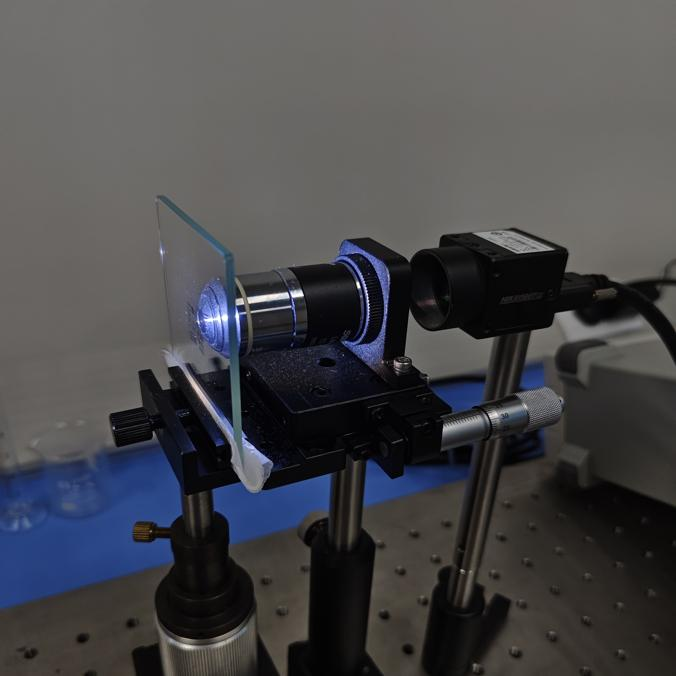
\includegraphics[width=\linewidth]{标定装置.jpg}
        \caption{装置图}
    \end{subfigure}
    \begin{subfigure}{0.45\textwidth}
        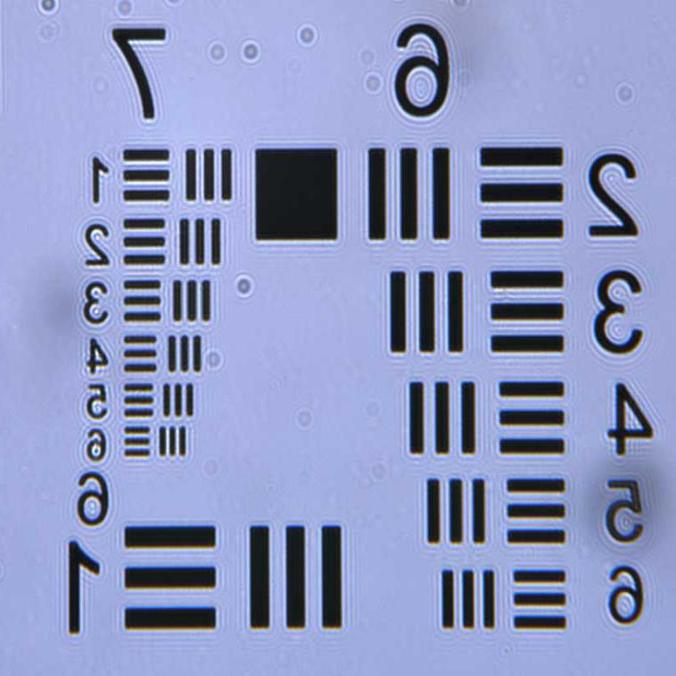
\includegraphics[width=\linewidth]{标定.jpg}
        \caption{拍摄到的部分分辨率板}
    \end{subfigure}

    \caption{标定}
    \label{fig:biaoding}
\end{figure}
2.配制适当浓度的不同直径(0.5~$\mu$m,2~$\mu$m,5~$\mu$m)、不同液体粘度(甘油与去离子水的混合)的聚苯乙烯(PS)微球。\par
剪取两片铜片作为电极,使用无水乙醇清洗后晾干。\par
3.将溶液加入比色皿中,放在夹具上静置 0.5--1 h。\\ 
\quad \textbullet\ 对于验证布朗运动的实验,无需插入电极、连接信号发生器等操作。 \\
\quad \textbullet\ 对于验证等效温度与扩散系数的拟合实验,插入电极并连接信号发生器,保持电极平行紧贴两侧。\par
4.开启 LED,观察 PS 微球,待稳定时收集数据(对于验证等效温度与扩散系数的拟合实验,在稳定后需要控制信号发生器
依次加载0--10V的电压,然后收集数据)。\par
5.将比色皿取下,拍摄背景图片。\par
6.进行数据处理,计算相关物理量。\\
下面是我们拍摄到的几个直径为0.5~$\mu$m的PS小球在去离子水中运动轨迹图和它在x方向上的位移随时间变化曲线:
\begin{figure}[H]
    \centering
    % 每行 2 张
    \begin{subfigure}{0.3\textwidth}
        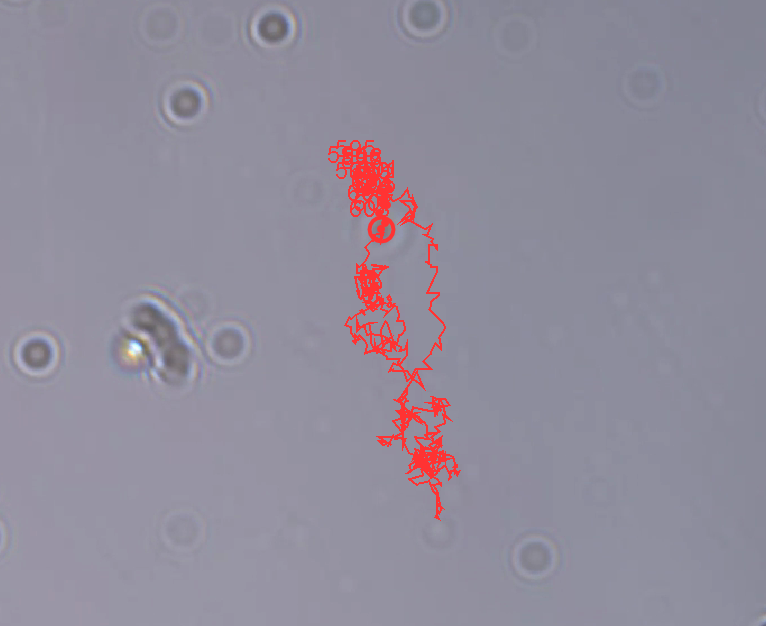
\includegraphics[width=\linewidth]{image1.png}
    \end{subfigure}
    \begin{subfigure}{0.6\textwidth}
        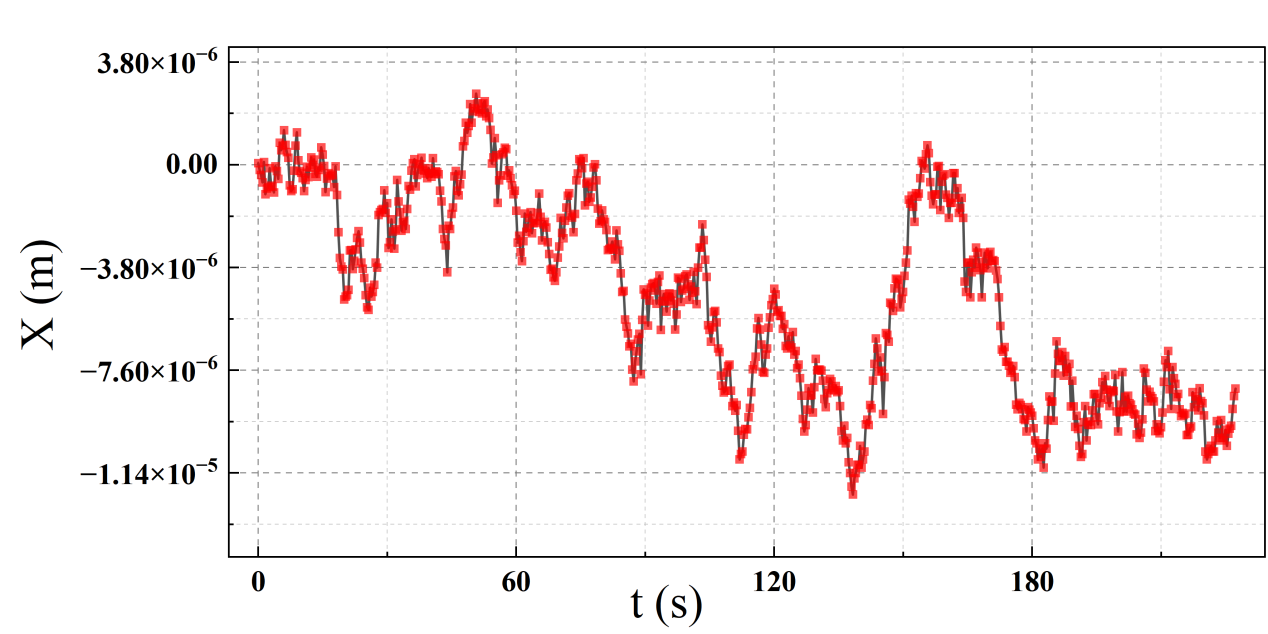
\includegraphics[width=\linewidth]{image2.png}
    \end{subfigure}

    \begin{subfigure}{0.3\textwidth}
        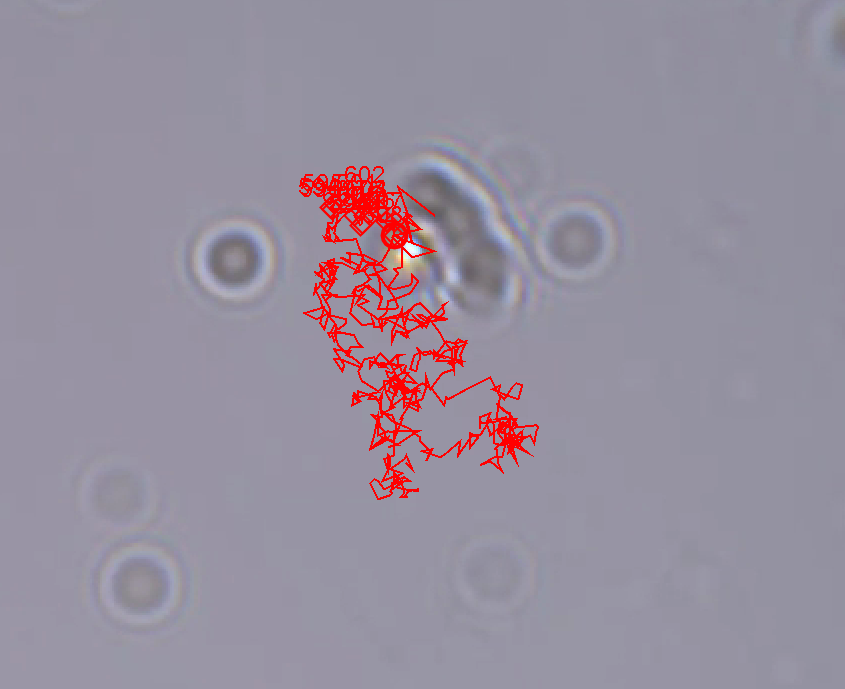
\includegraphics[width=\linewidth]{image3.png}
    \end{subfigure}
    \begin{subfigure}{0.6\textwidth}
        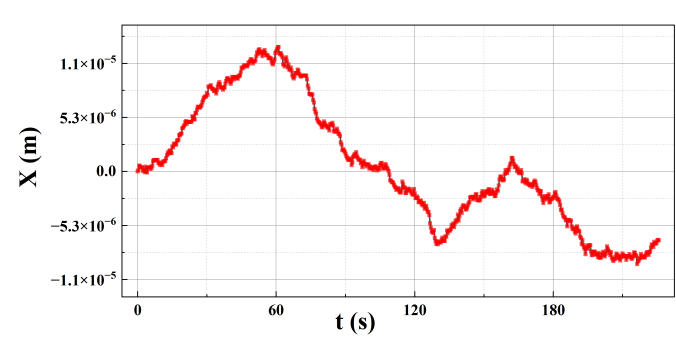
\includegraphics[width=\linewidth]{image4.png}
    \end{subfigure}

    \begin{subfigure}{0.3\textwidth}
        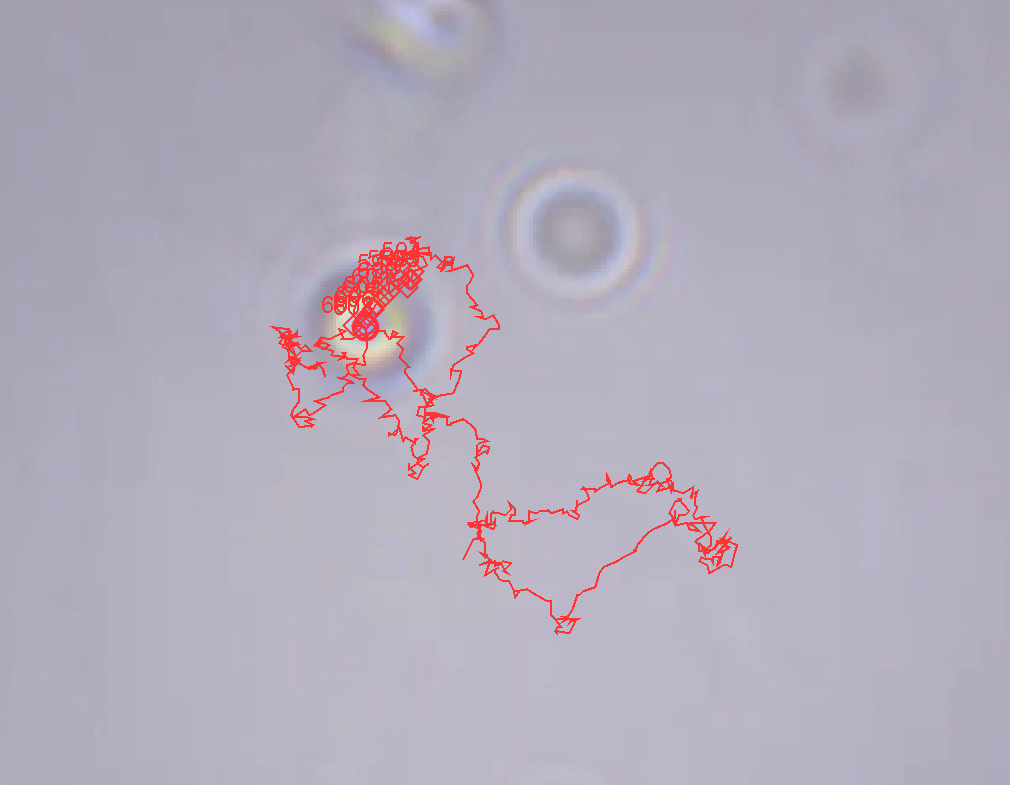
\includegraphics[width=\linewidth]{image5.png}
    \end{subfigure}
    \begin{subfigure}{0.6\textwidth}
        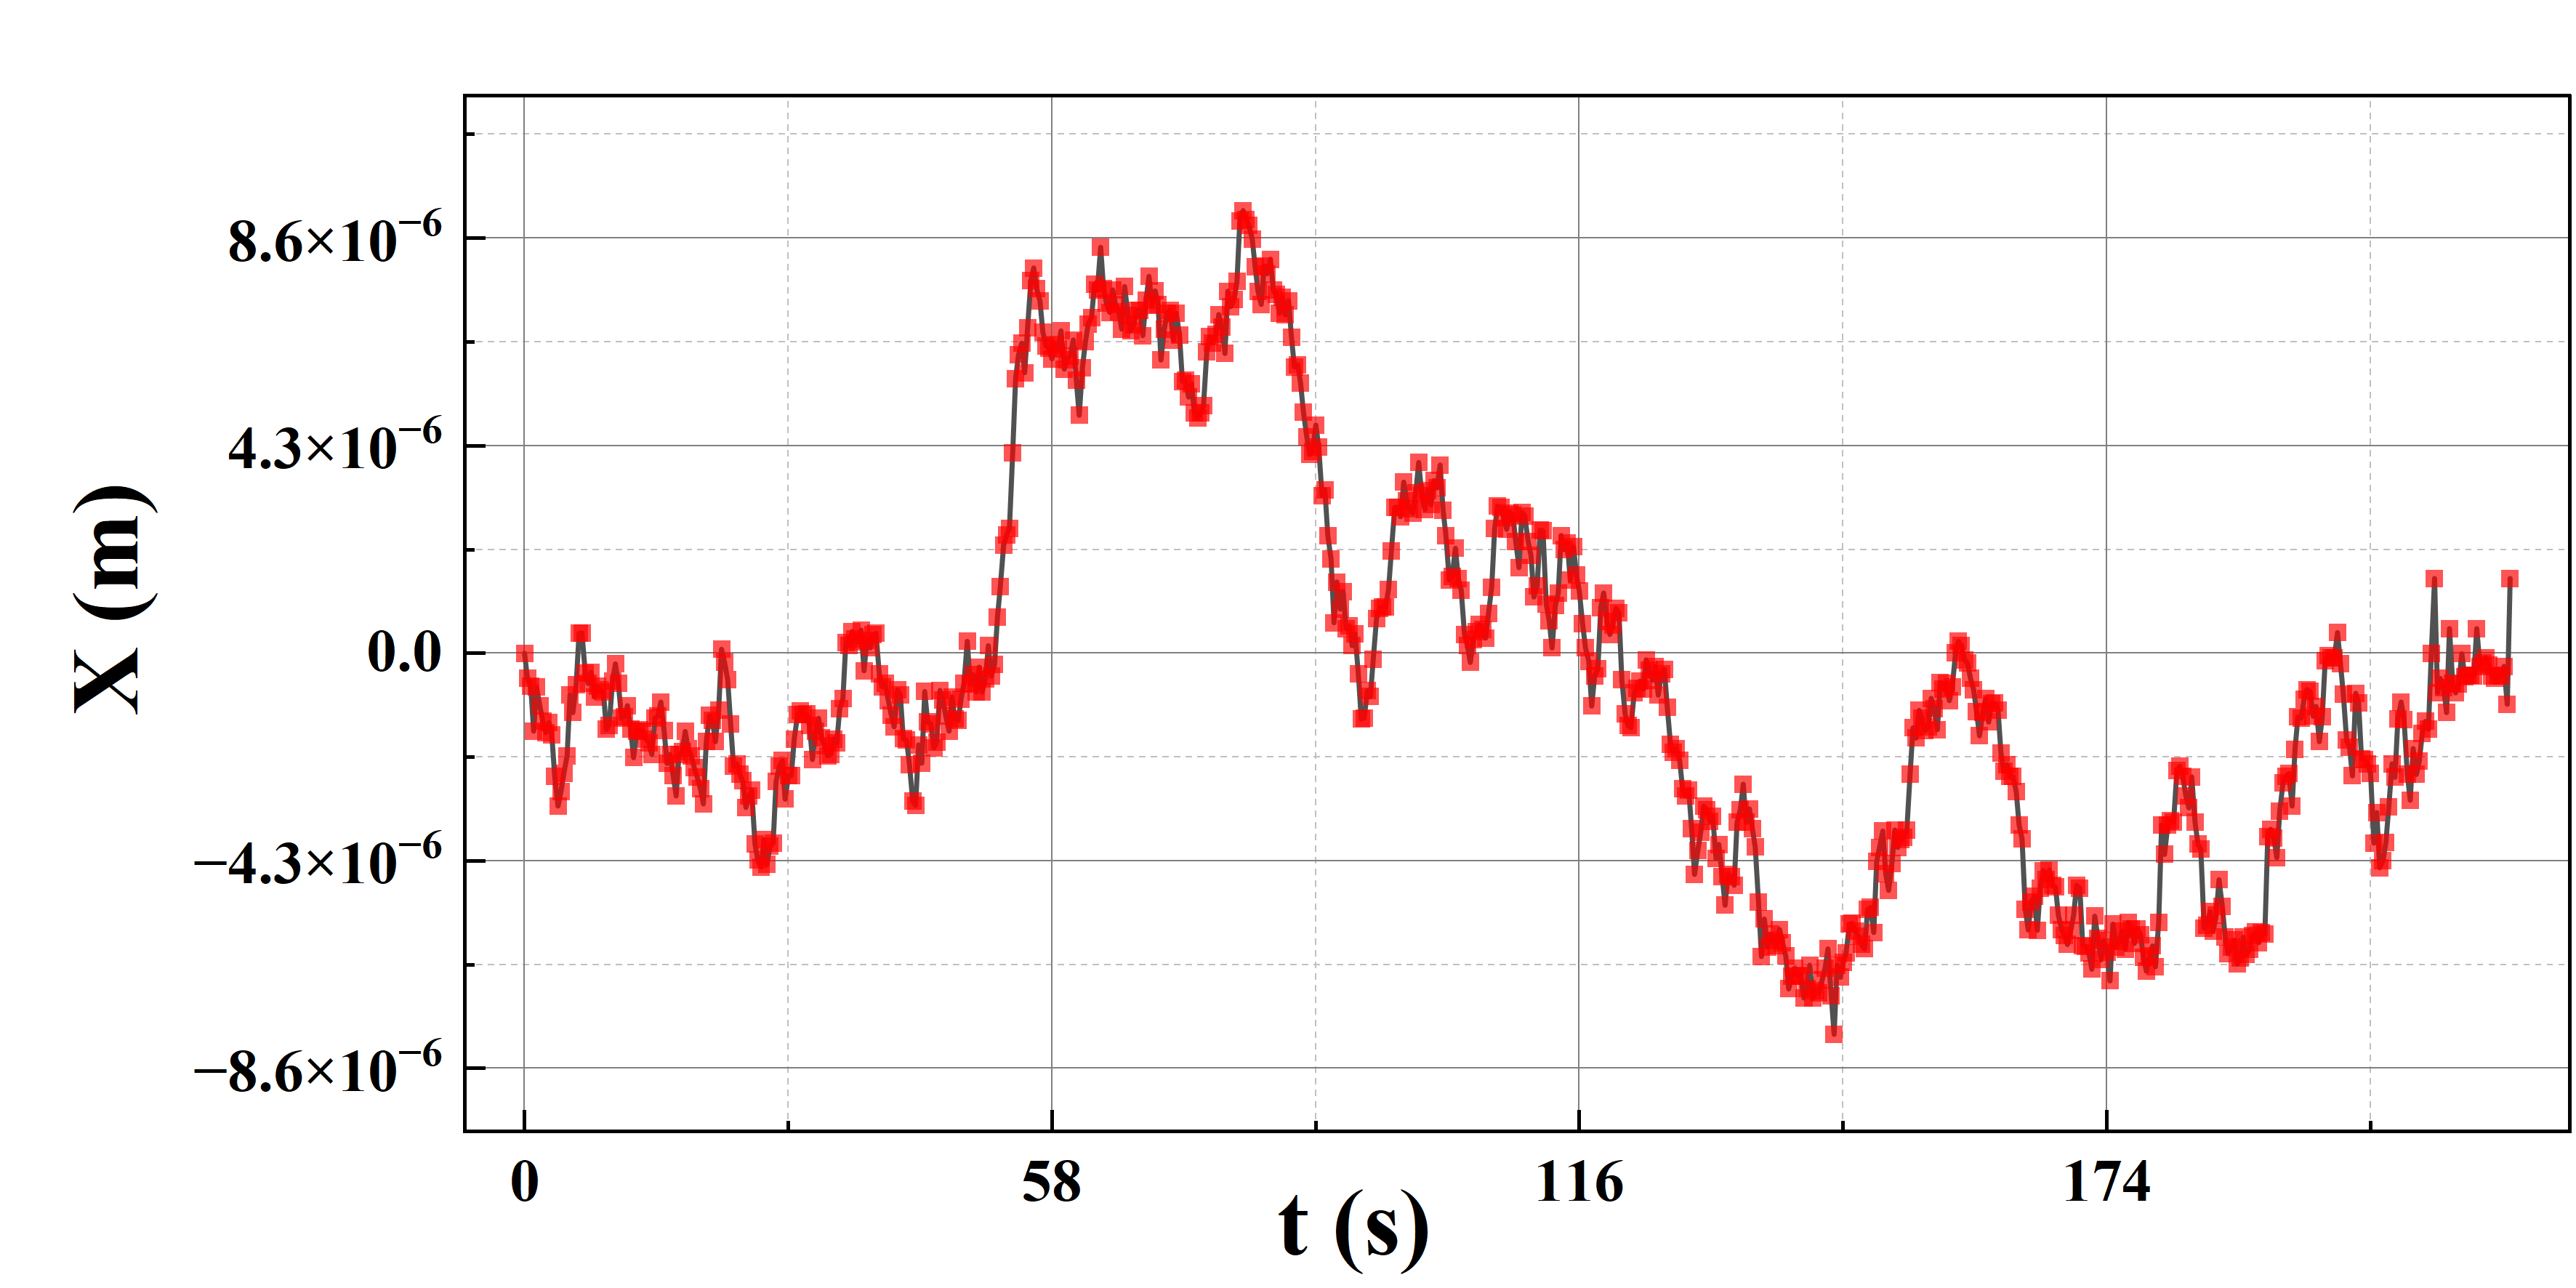
\includegraphics[width=\linewidth]{image6.png}
    \end{subfigure}

    \caption{0.5~$\mu$m微球轨迹图与位移-时间图像}
\end{figure}
\newpage
\subsection{数据处理}
1. 首先,使用附录~\ref{code:searchforparticles}的python代码对采集到的视频进行处理,提取出每一帧图像,并使用trackpy库对每一帧图像进行粒子检测,得到每一帧中所有粒子的坐标信息:\\
使用python提取视频,获得每一帧图像:\\
用python的cv2和os模块,来逐帧截取视频:
\begin{figure}[H]
    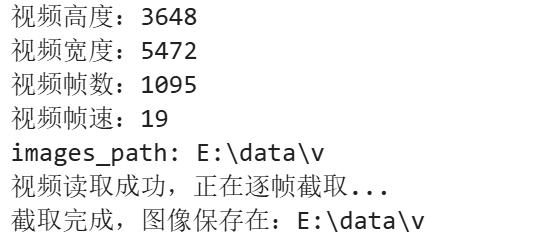
\includegraphics[width=0.6\textwidth]{说明.png}
\end{figure} 
\begin{figure}[H]
    \centering
    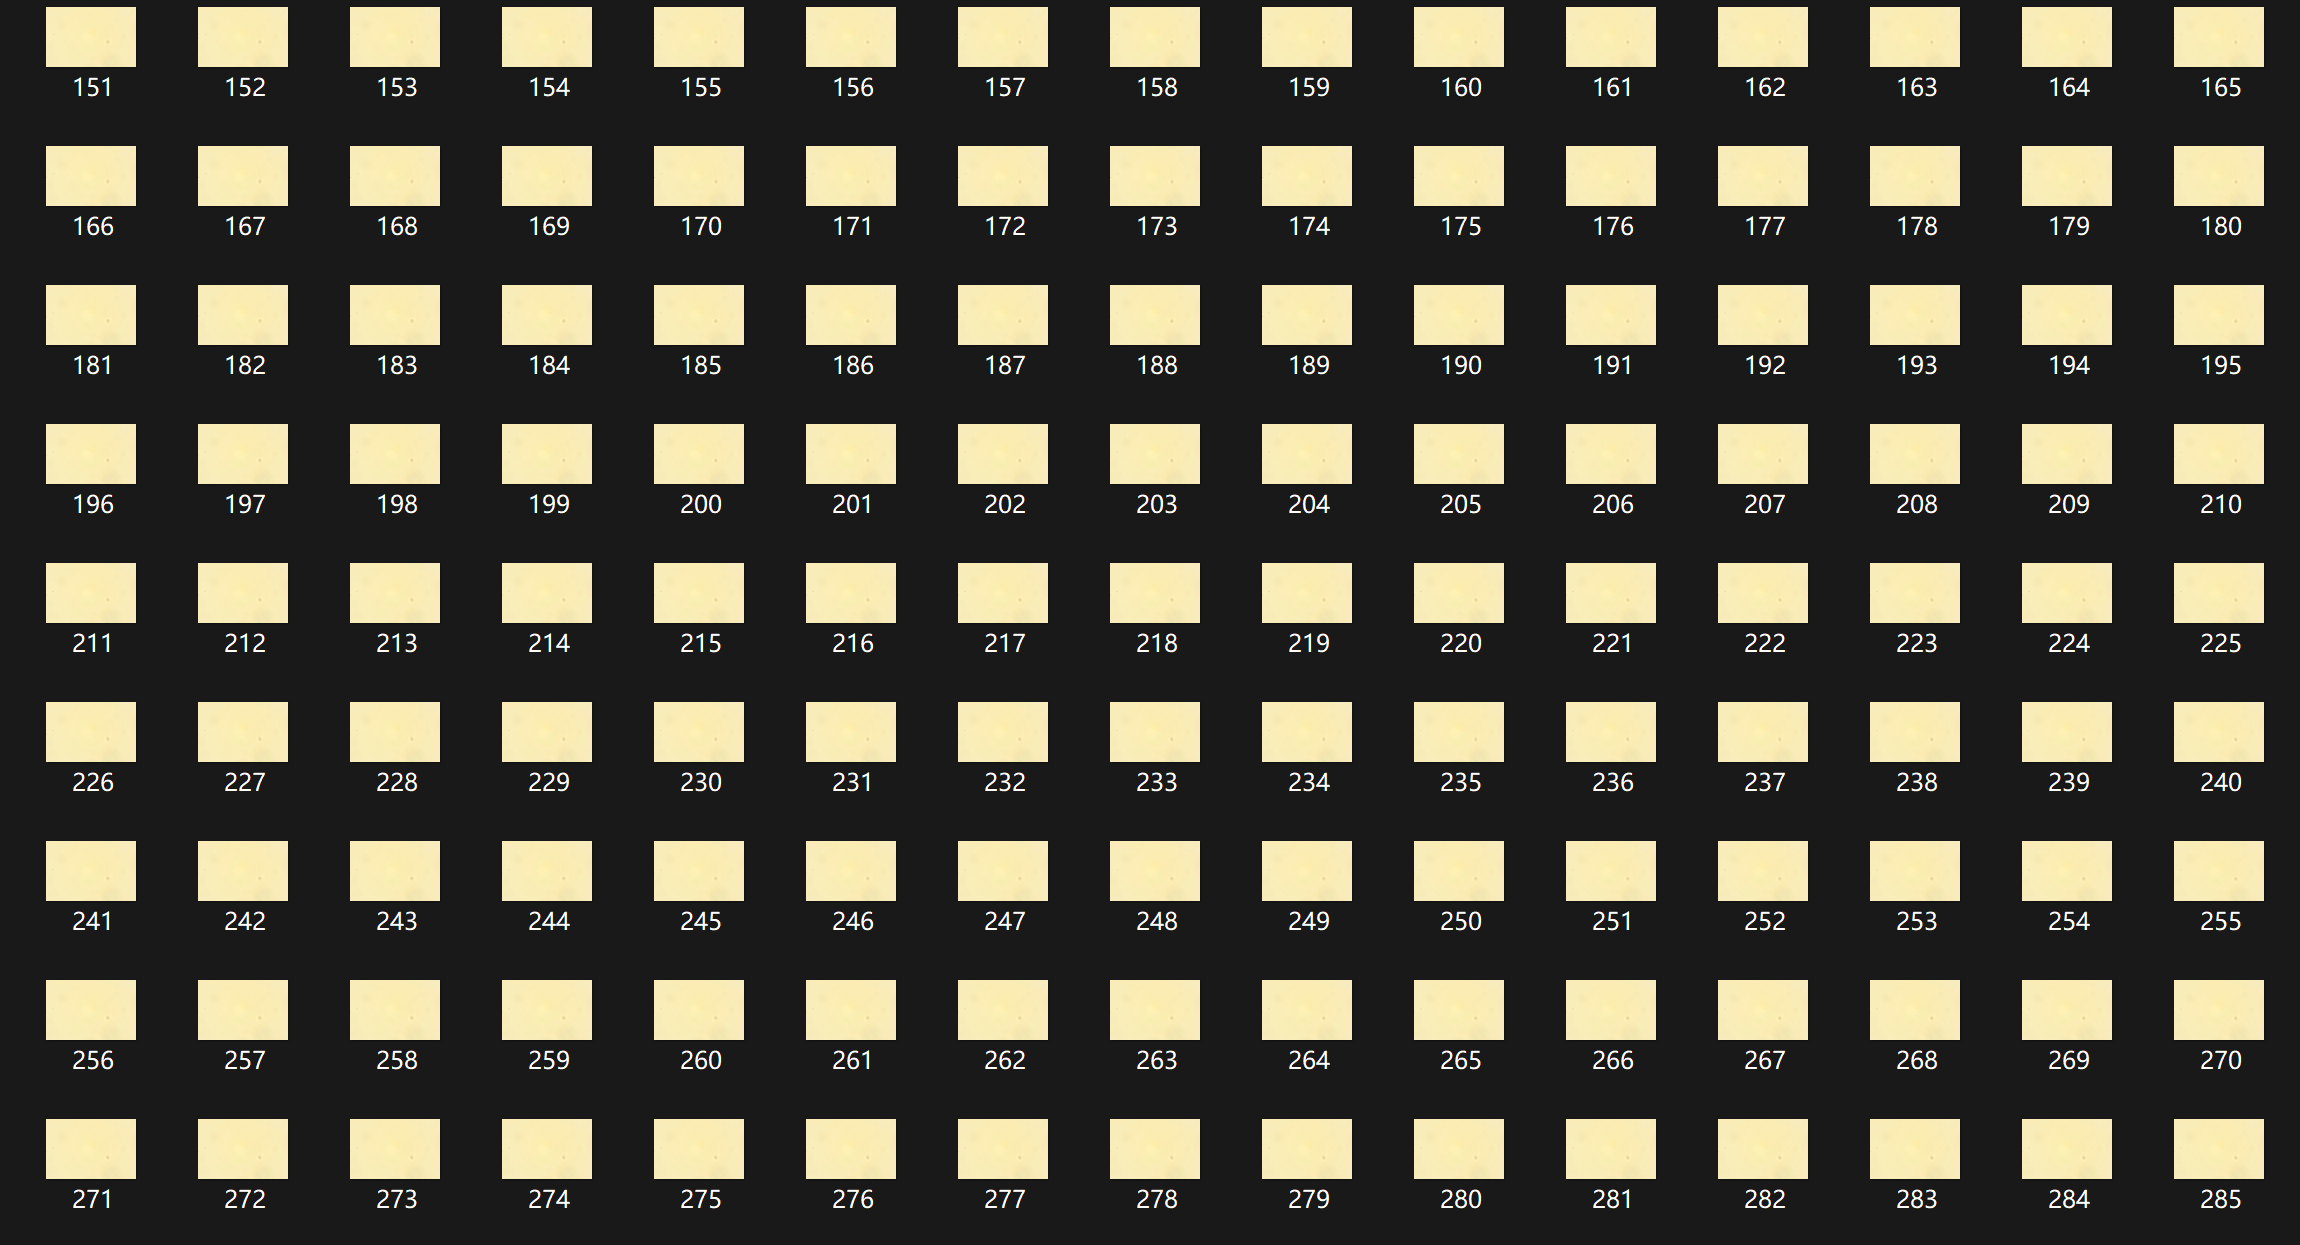
\includegraphics[width=0.8\textwidth]{图片.png}
    \caption{截取图片}
\end{figure} 
背景图像去除防止干扰,增强对比度,并使用标准的RGB转灰度公式将每一帧图片其转换为灰度图像:\\
\begin{figure}[H]
    \centering
    % 每行 2 张
    \begin{subfigure}{0.45\textwidth}
        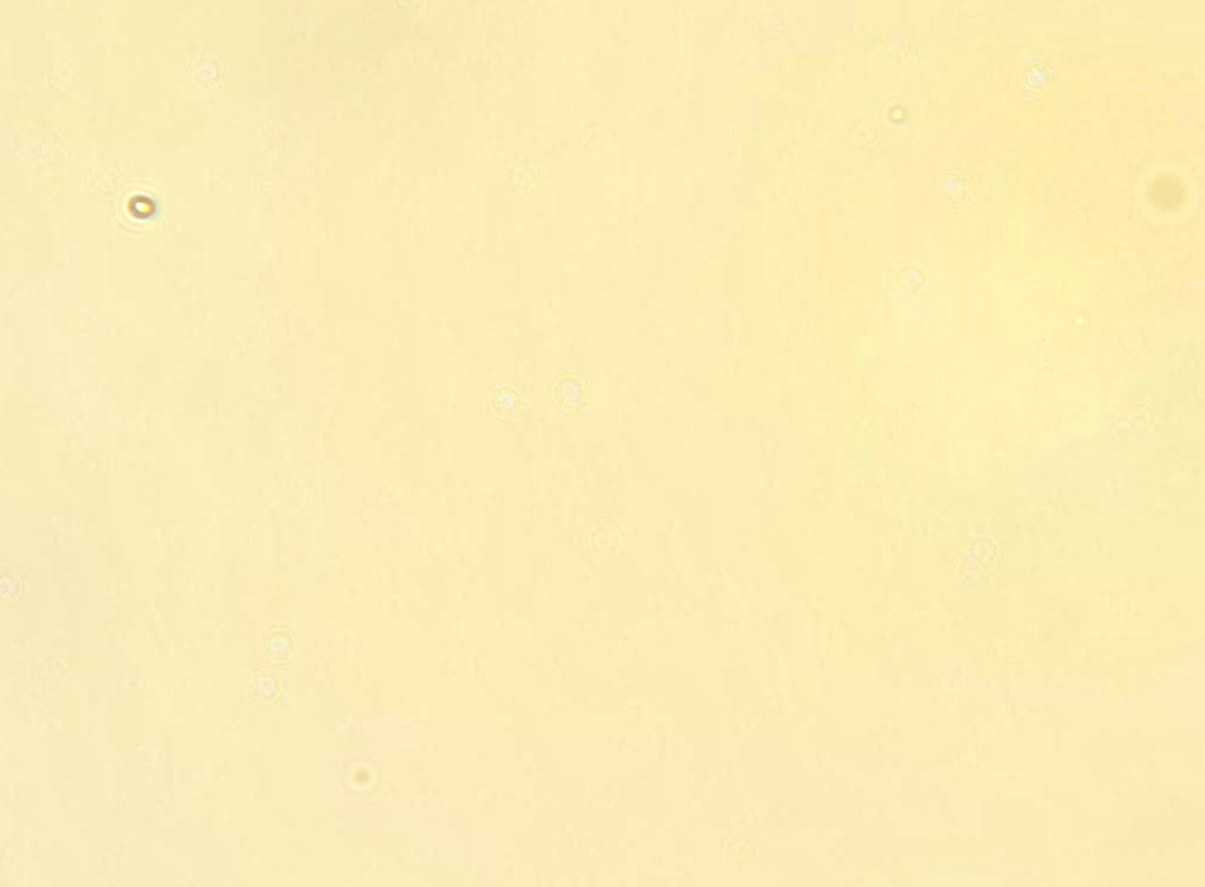
\includegraphics[width=\linewidth]{去背景.png}
        \caption{去背景}
    \end{subfigure}
    \begin{subfigure}{0.45\textwidth}
        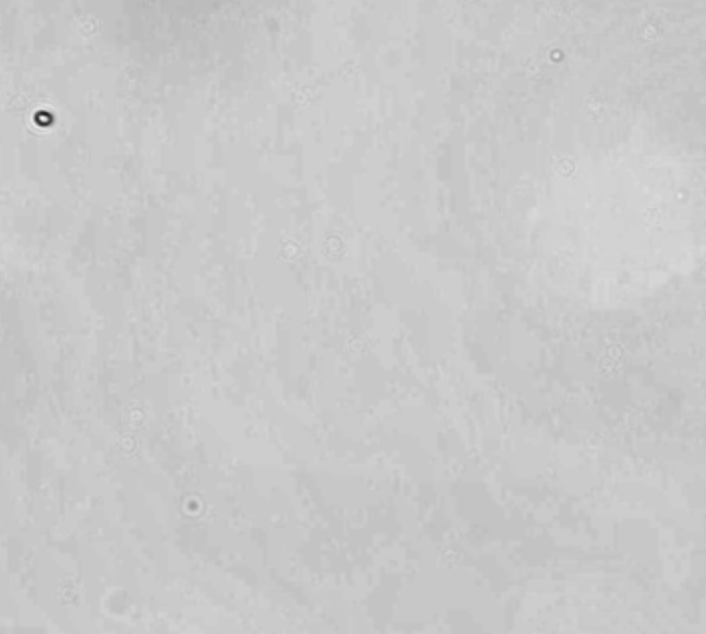
\includegraphics[width=\linewidth]{转灰度.png}
        \caption{转灰度}
    \end{subfigure}

    \caption{去背景并转灰度}
\end{figure}
2. 对粒子进行识别:\\
使用trackpy中的locate函数来检测图像中可能的粒子(圆形高斯拟合)
检测直径比实际例子直径稍大些所对应像素大小的亮/暗粒子(与背景有关)
包含所有检测到粒子的信息(坐标、强度、椭圆度等)
使用trackpy中的annotate函数来标注检测到的粒子(可以通过调整minmass参数、maxsize参数和separation参数来限制粒子的强度、例子最大尺寸和粒子间的最小间隔)
\begin{figure}[H]
    \centering
    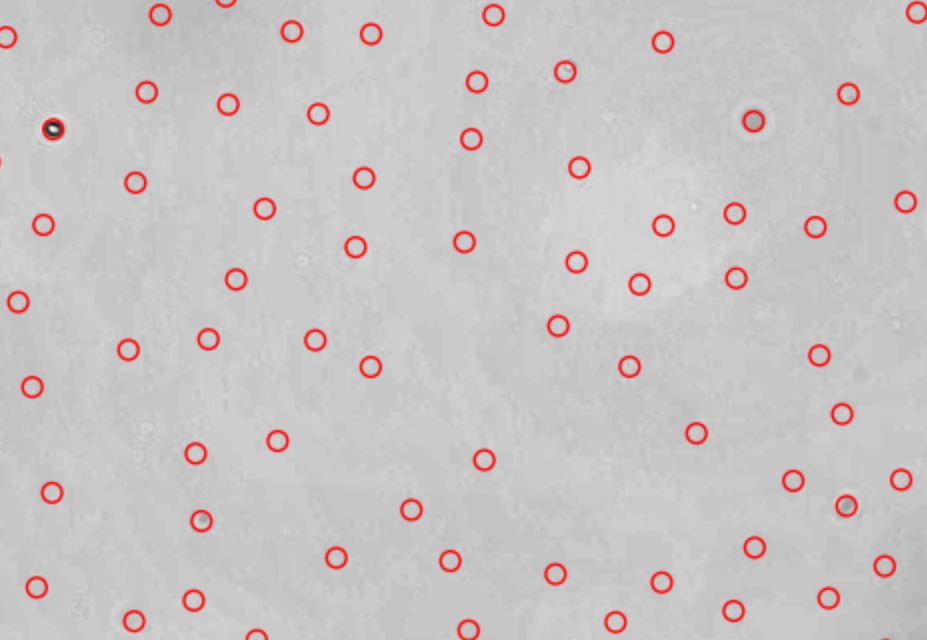
\includegraphics[width=0.8\textwidth]{识别粒子.png}
    \caption{检测并识别粒子}
\end{figure} 
3. 对所有帧中的粒子进行追踪,得到每个粒子的轨迹信息。\\
粒子位置的提取(如图~\ref{fig:guijitu})x,y(本实验中y为竖直方向坐标,本实验只考虑一维x方向坐标所)位置坐标,mass表示粒子亮度。
\begin{figure}[H]
    \centering
    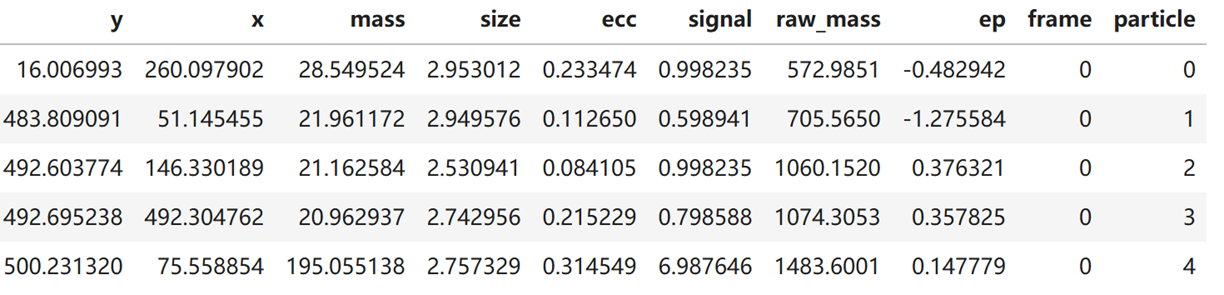
\includegraphics[width=0.8\textwidth]{粒子信息.png}
    \caption{粒子信息示例}
\end{figure} 
\begin{figure}[H]
    \centering
    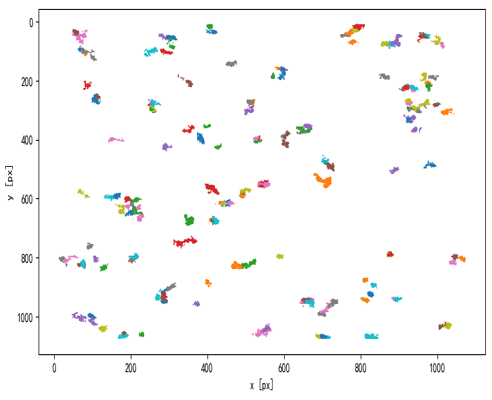
\includegraphics[width=0.8\textwidth]{粒子轨迹图.png}
    \caption{粒子运动轨迹识别}
    \label{fig:guijitu}
\end{figure} 
4. 计算每个粒子的MSD:使用tp.imsd函数来计算单粒子的均方位移(MSD)
\begin{figure}[H]
    \centering
    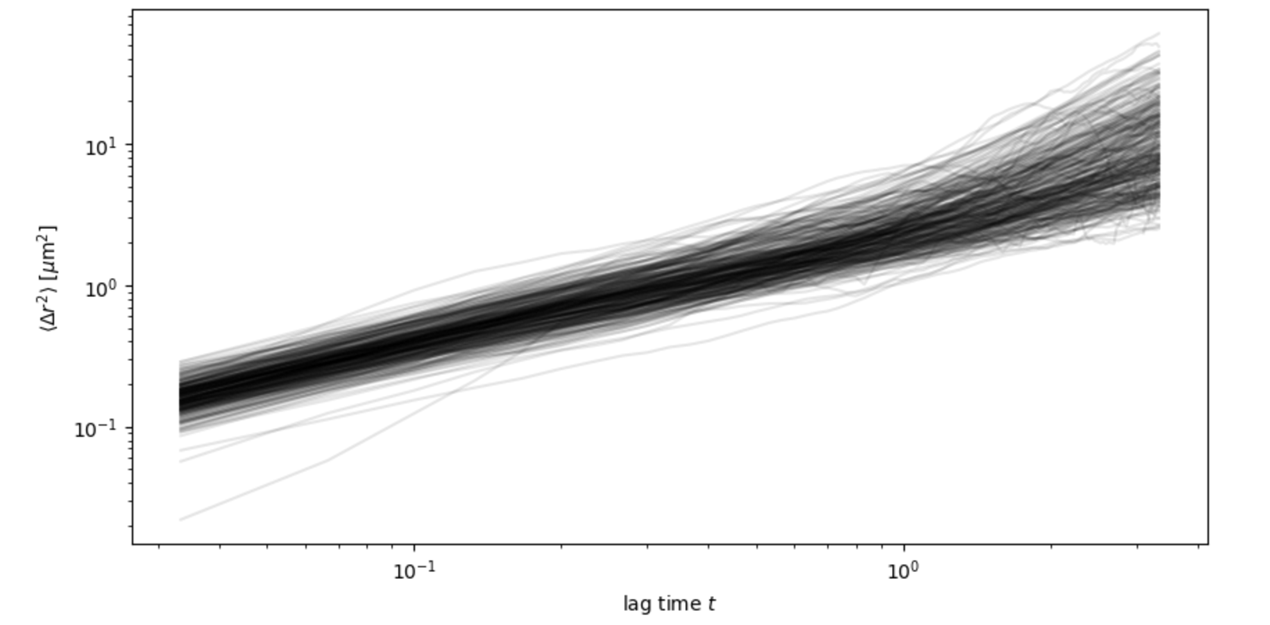
\includegraphics[width=0.8\textwidth]{计算MSD.png}
    \caption{计算MSD}
\end{figure} 
5. 在本实验的探究过程中,粒子进行布朗运动时,其均方位移(MSD)满足关系式:
$\langle r(t)^2 \rangle = 2Dt,$其中 $D$ 为扩散系数。由此可知,MSD--时间曲线应当呈现线性关系,拟合所得直线斜率为
$A = 2D.$在实际数据处理中,我们使用 \texttt{tp.emsd} 函数来计算群体平均 MSD 曲线。
\begin{figure}[H]
    \centering
    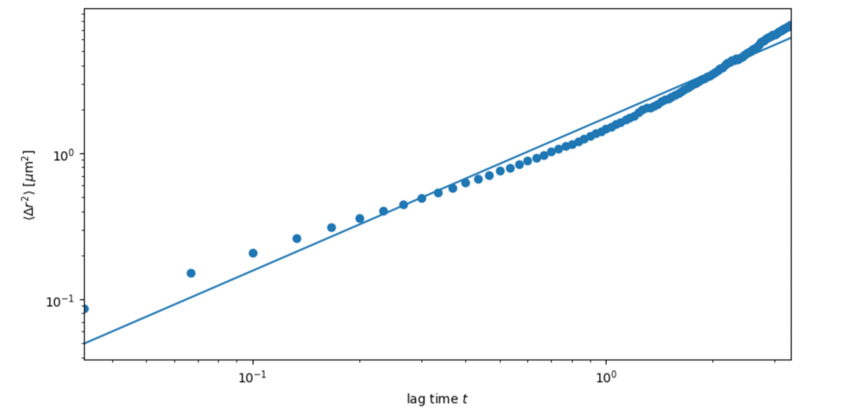
\includegraphics[width=0.8\textwidth]{计算并拟合.png}
    \caption{计算并拟合}
\end{figure} 
6. 获得实验值与理论值的对比数据图,以及某个粒子的位移变化图:
\begin{figure}[H]
    \centering
    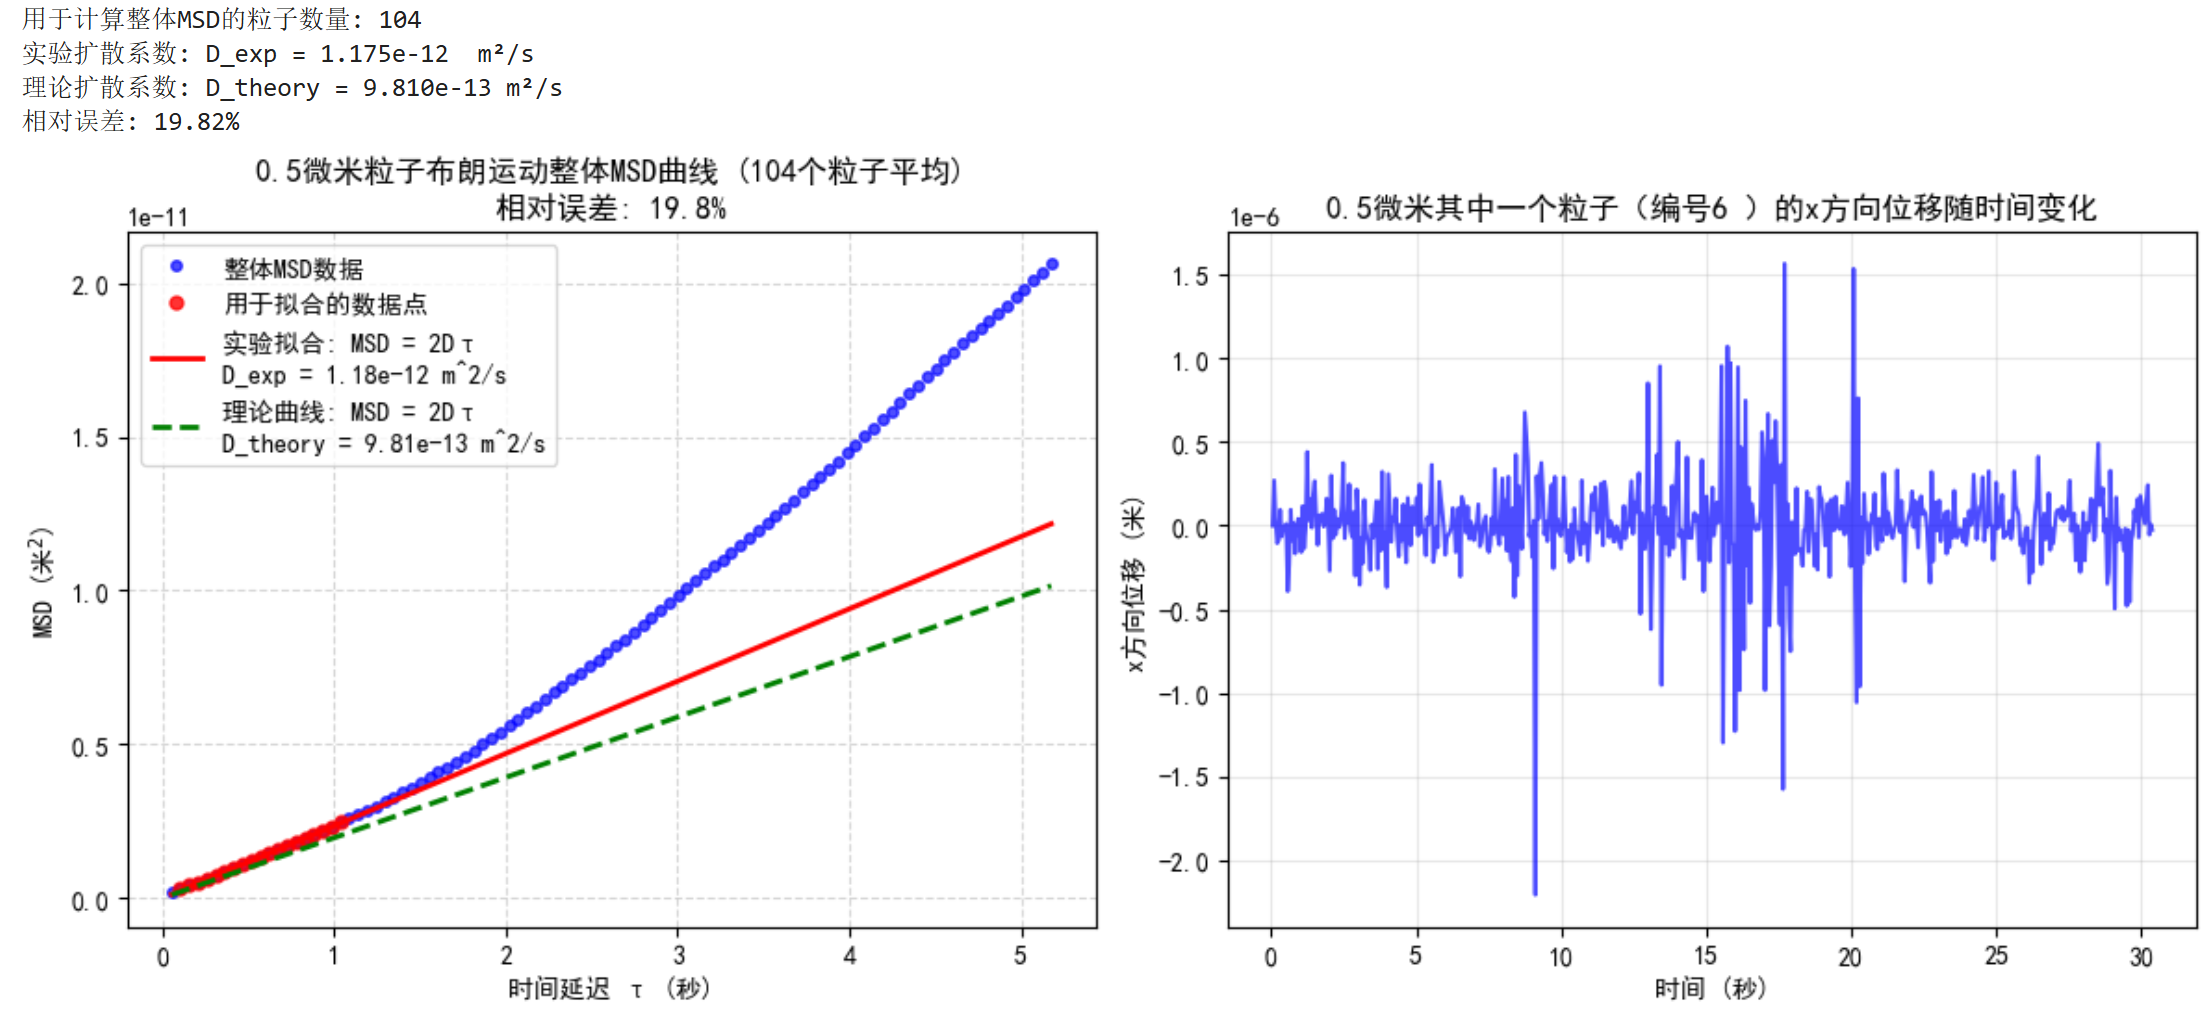
\includegraphics[width=0.8\textwidth]{实际示例.png}
    \caption{实验与理论对比}
\end{figure} 
函数实现参考了 GitHub 项目 \emph{trackpy: Python particle tracking toolkit}\footnote{\url{https://github.com/soft-matter/trackpy}}。
\section{MSD与时间t的线性关系验证}
首先根据前面处理得到的MSD数据绘制MSD与时间t的关系图,并对数据进行线性拟合(只取时间间隔为0-1s的数据进行拟合,具体的原因详见附录:有效拟合区间的选取与图~\ref{fig:let1}。对于本实验可以得到只有时间间隔在0-1s内才是误差可接受的范围。后续没有特殊说明时,拟合MSD均取0-1s),
验证MSD与时间t的线性关系。 \par
\subsection{不同直径粒子的均方位移(MSD)}
\begin{figure}[H]
  \centering
  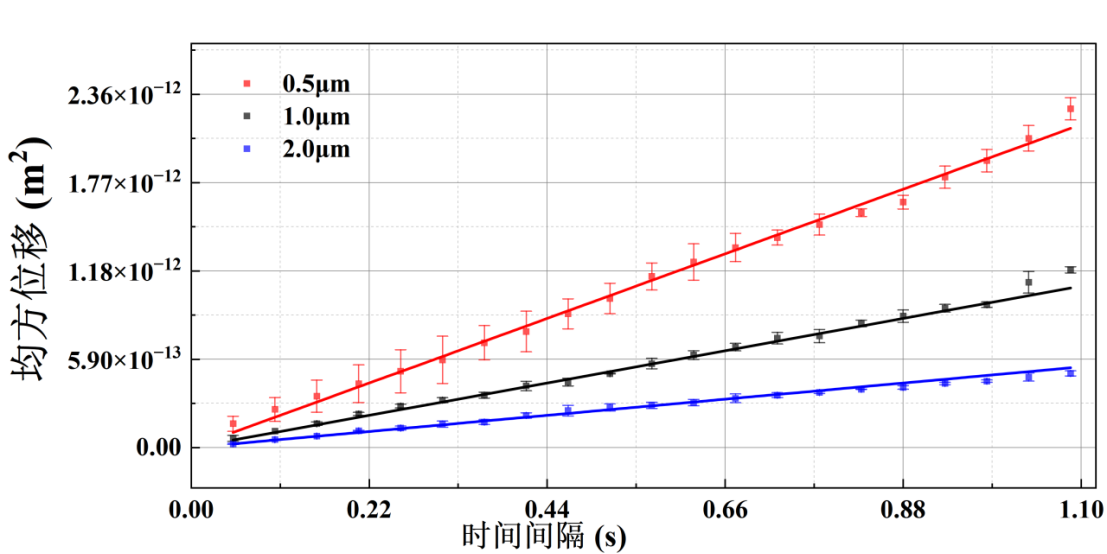
\includegraphics[width=0.7\textwidth]{实验数据拟合1.png}
  \caption{不同粒径的实验MSD与拟合曲线以及局部放大图,以及扩散系数}
  \label{fig:fit1}
\end{figure}
\begin{table}[H]
\centering
\begin{tabular}{cccc}
\hline
粒径 & 扩散系数实验值 ($\mathrm{m^2/s}$) & 扩散系数理论值 ($\mathrm{m^2/s}$) & 相对误差 \\
\hline
0.5 $\mu$m & $9.809 \times 10^{-13}$ & $9.81 \times 10^{-13}$ & 0.01\% \\
1.0 $\mu$m & $5.0602 \times 10^{-13}$ & $4.91 \times 10^{-13}$ & 3.1\% \\
2.0 $\mu$m & $2.354885 \times 10^{-13}$ & $2.45 \times 10^{-13}$ & 3.9\% \\
\hline
\end{tabular}
\caption{不同粒径下实验与理论扩散系数对比}
\end{table}

得到上面的数据后,可以将实验所得的扩散系数与理论值进行对比。根据
\begin{equation}
    D = \frac{k_B T}{6 \pi \eta r},
\end{equation}
在其他条件不变的情况下,粒子直径越大,其扩散系数越小。通过对不同粒径布朗粒子在前段较稳定的 MSD 进行拟合,可以发现三种粒子的扩散系数满足
\[
    D_{0.5} > D_{2.0} > D_{5.0}.
\]

\subsection{不同粘度溶液中的均方位移(MSD)}
在20\%浓度的甘油中,我们截取其中一个微球的运动轨迹和位移-时间图像如下:\par
\begin{figure}[H]
    \centering
    % 每行 2 张
    \begin{subfigure}{0.3\textwidth}
        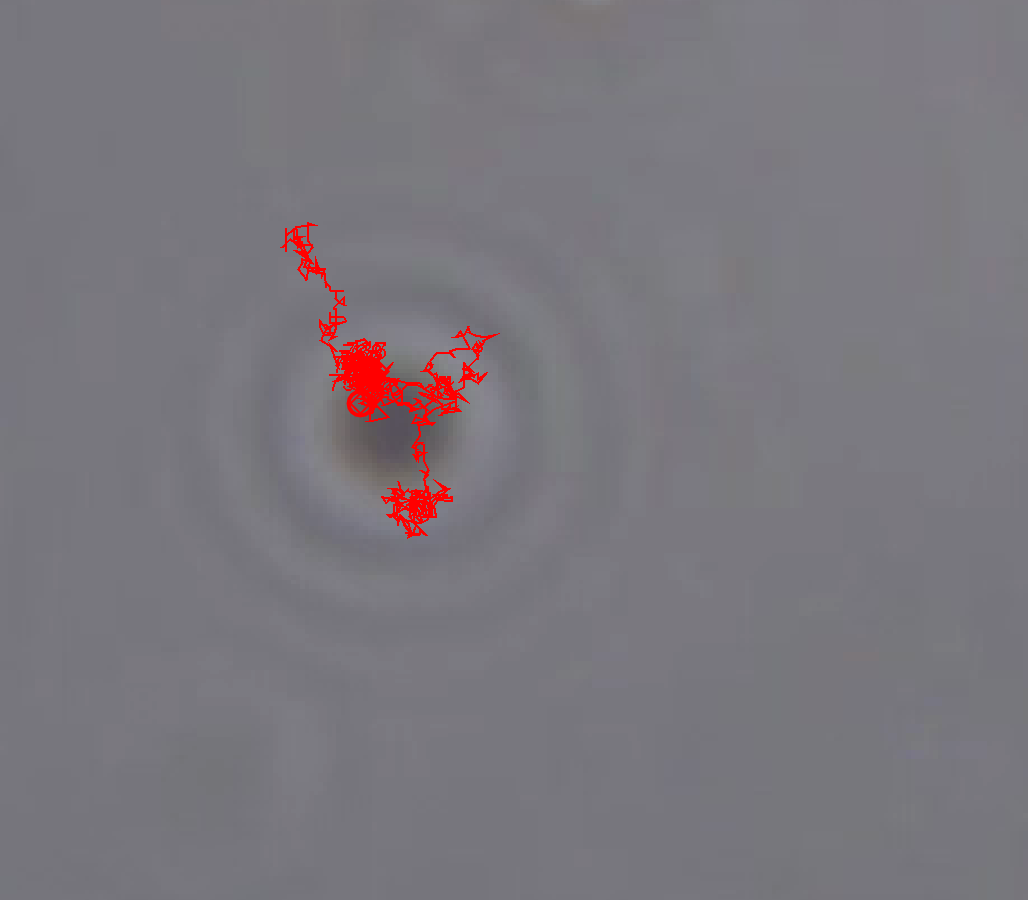
\includegraphics[width=\linewidth]{image7.png}
    \end{subfigure}
    \begin{subfigure}{0.6\textwidth}
        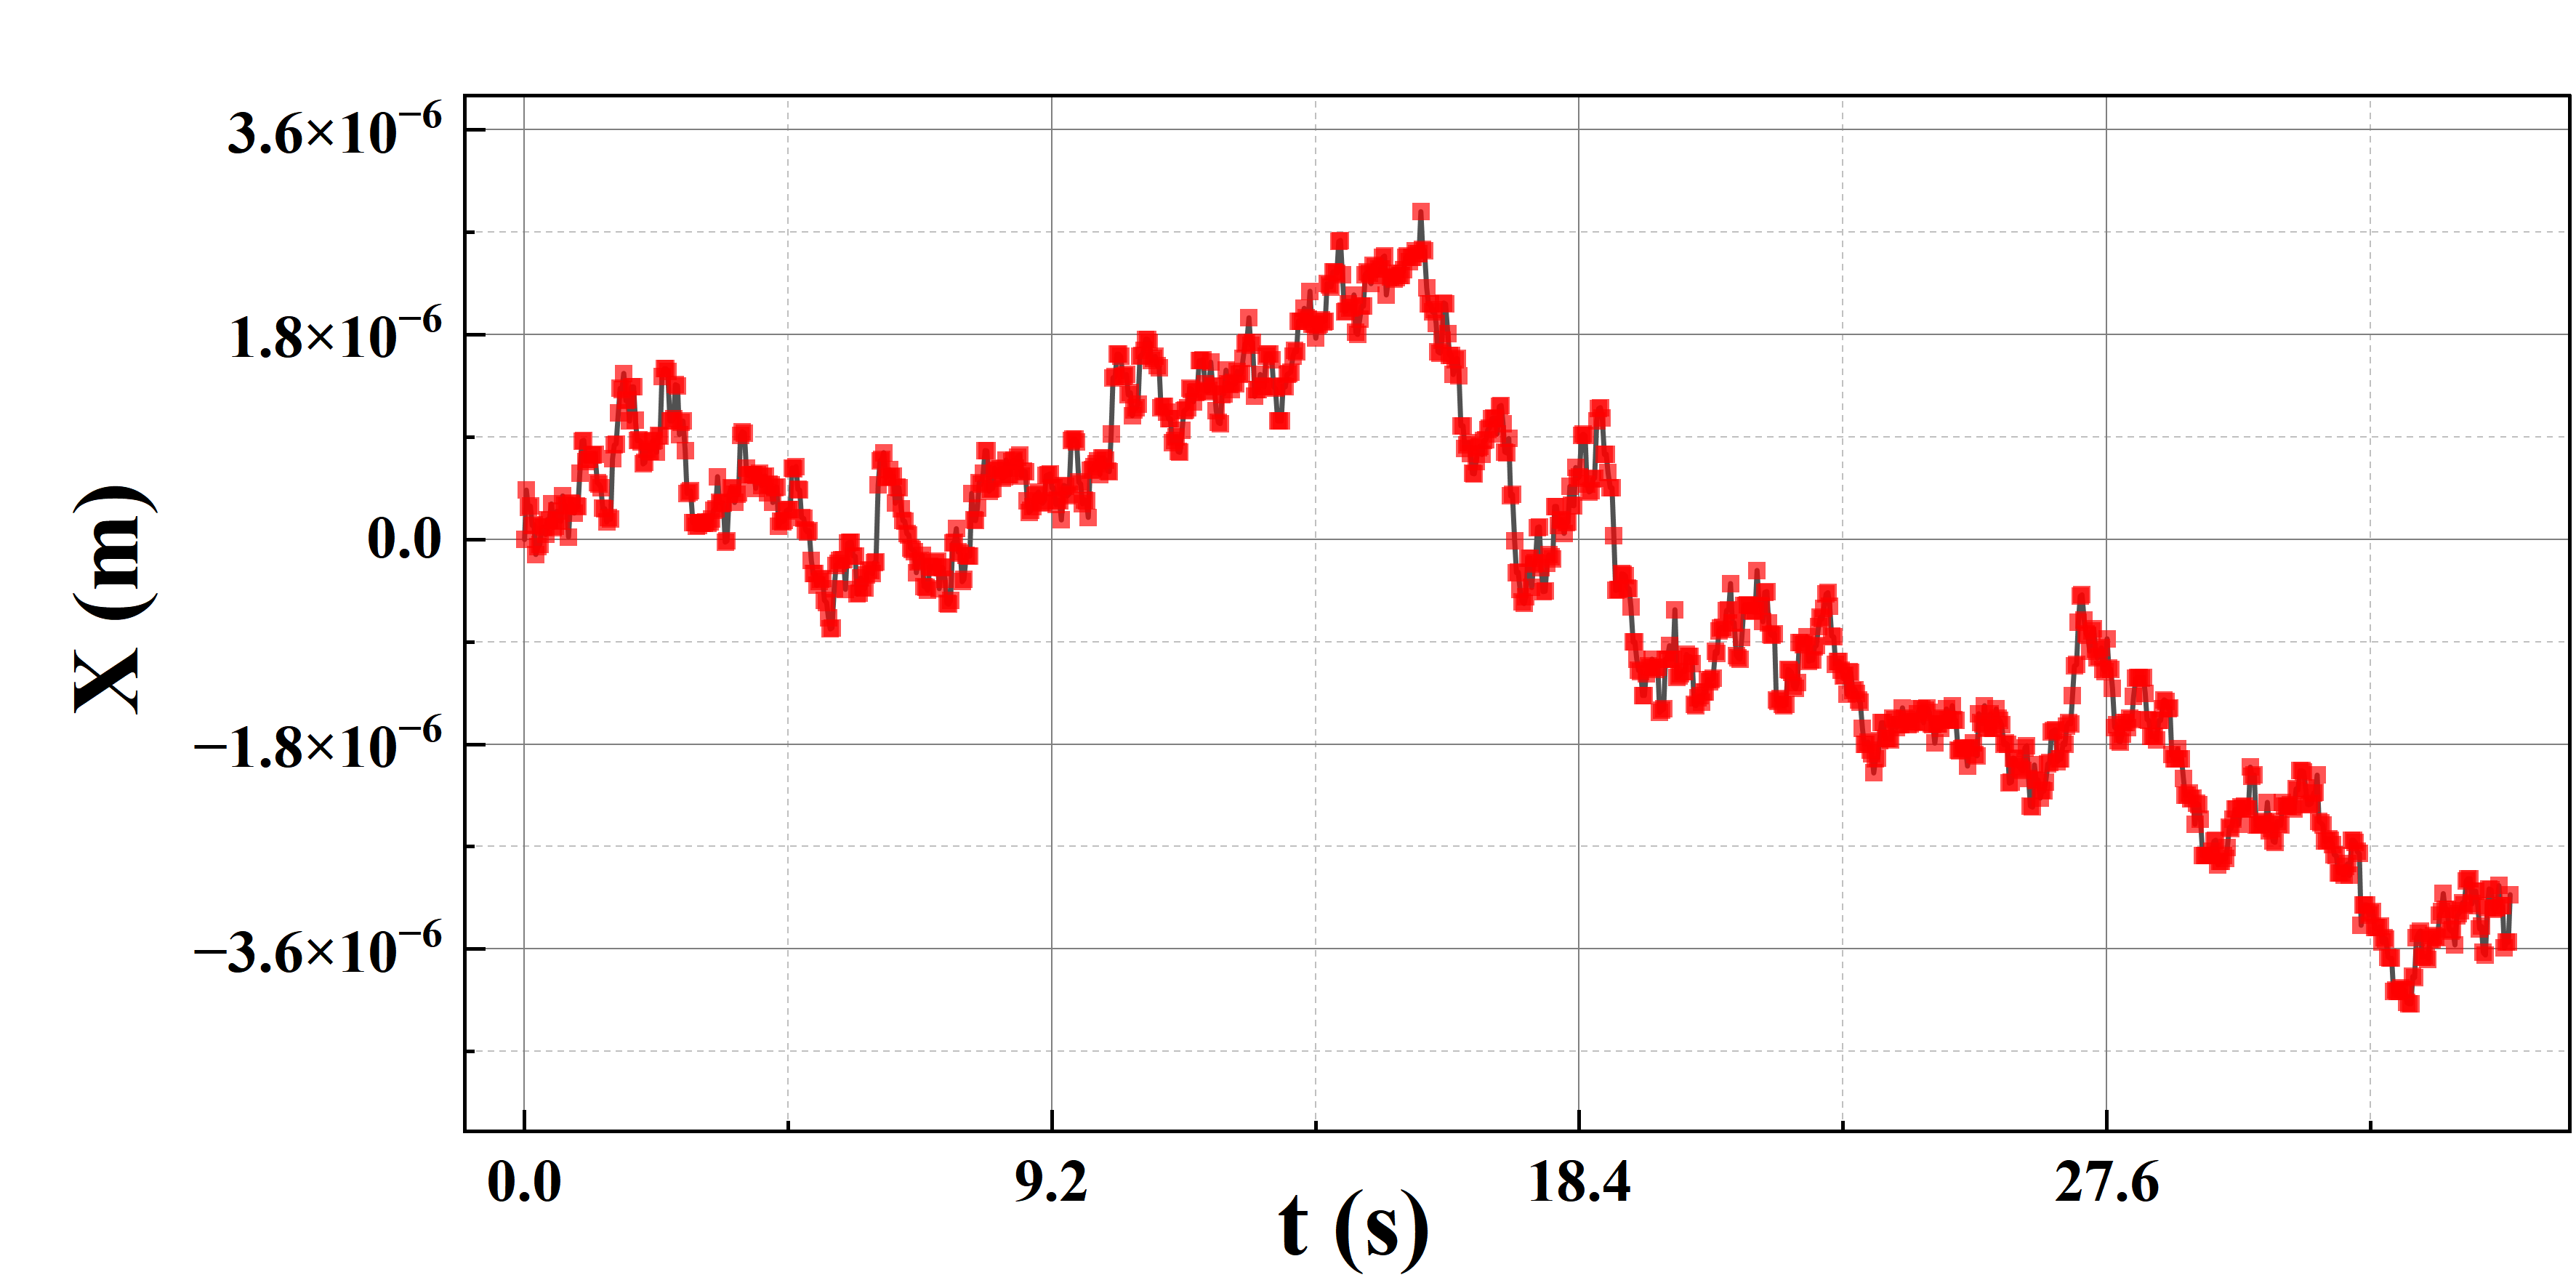
\includegraphics[width=\linewidth]{image8.png}
    \end{subfigure}

    \caption{0.5~$\mu$m的粒子在20\%粘度溶液中的运动轨迹和x-t图}
\end{figure}
我们分别配制了不同比例(甘油分别为10\%,15\%,20\%,30\%)的甘油与去离子水混合溶液,测量了不同粘度下0.5~$\mu$m的MSD,并画出了理论线:\par
\begin{figure}[H]
    \centering
    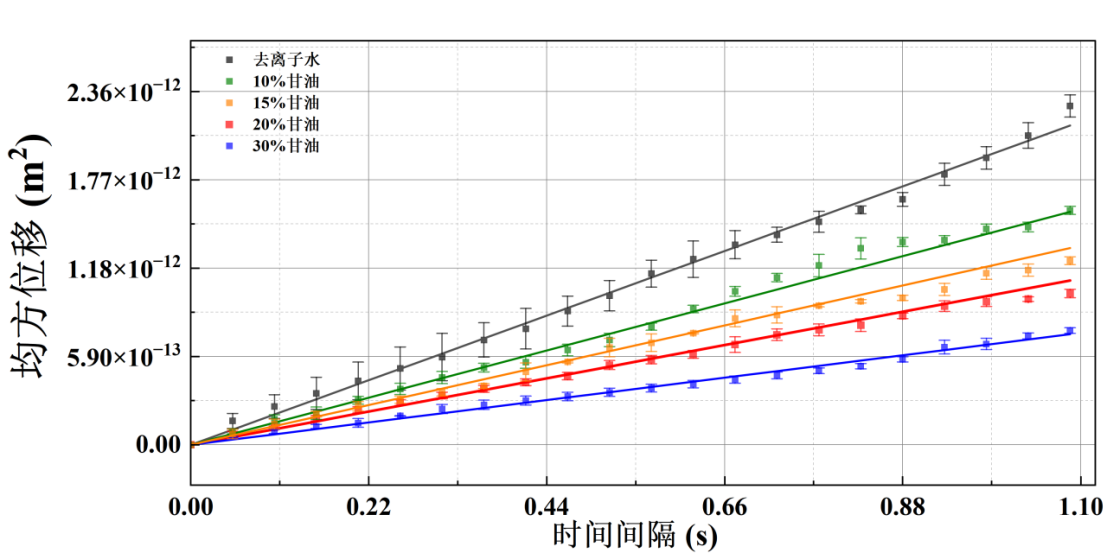
\includegraphics[width=0.8\linewidth]{实验数据拟合2.png}
    \caption{0.5~$\mu$m的粒子在不同粘度溶液中的MSD}
    \label{fig:fit2}
\end{figure}
\begin{table}[H]
\centering
\begin{tabular}{cccc}
\hline
甘油体积分数 & 扩散系数实验值 ($\mathrm{m^2/s}$) & 扩散系数理论值 ($\mathrm{m^2/s}$) & 相对误差 \\
\hline
0\%  & $9.87447 \times 10^{-13}$ & $9.81 \times 10^{-13}$ & 0.66\% \\
10\% & $7.3533 \times 10^{-13}$  & $7.16 \times 10^{-13}$ & 2.7\%  \\
15\% & $5.804 \times 10^{-13}$   & $6.05 \times 10^{-13}$ & 4.1\%  \\
20\% & $4.88932 \times 10^{-13}$ & $5.05 \times 10^{-13}$ & 3.2\%  \\
30\% & $3.38662 \times 10^{-13}$ & $3.40 \times 10^{-13}$ & 0.40\% \\
\hline
\end{tabular}
\caption{不同甘油体积分数下实验与理论扩散系数对比}
\end{table}

\section{计算等效温度与扩散系数}
对于加载不同噪声强度的实验,我们以0.5~$\mu$m的粒子为例,为了验证我们能够将信号发生器的电压加载到电极并且对微球产生影响,我们
在进行正式实验之前,先加载了正弦波与方波来进行验证:\par
\begin{figure}[H]
    \centering
    % 每行 2 张
    \begin{subfigure}{0.25\textwidth}
        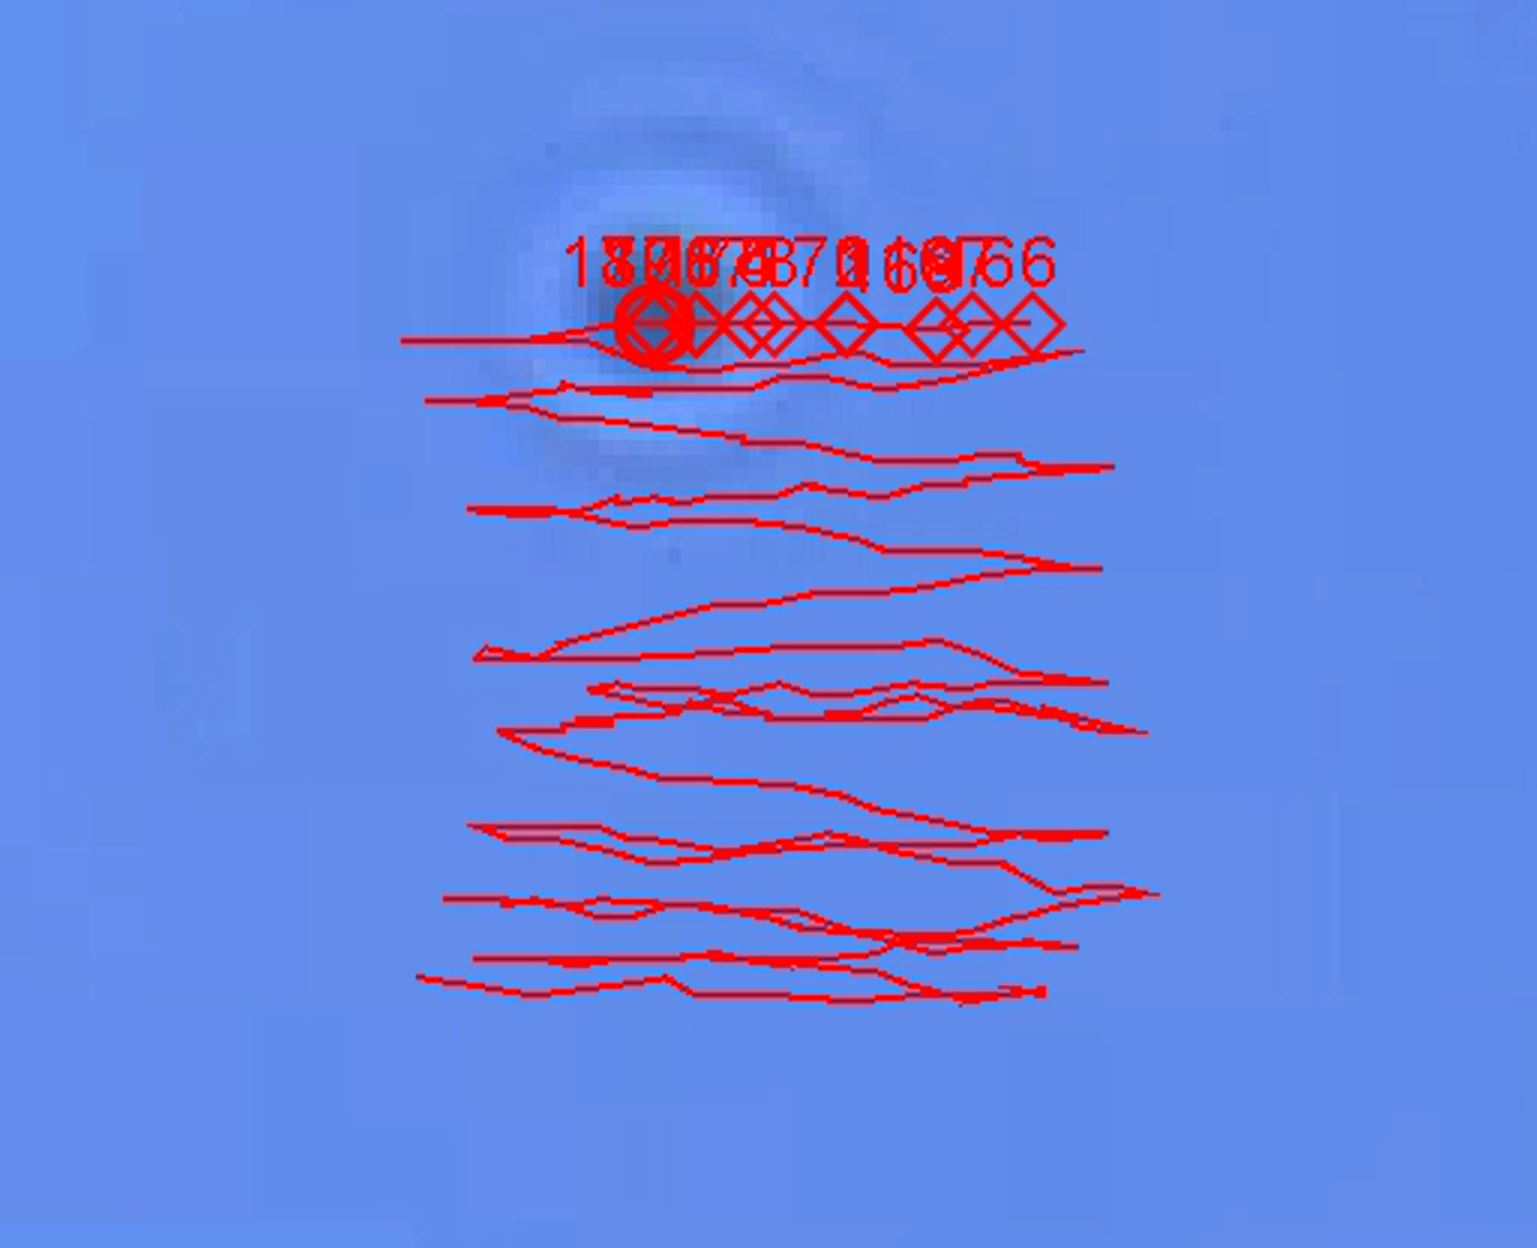
\includegraphics[width=\linewidth]{10v0.5Hz.png}
        \caption{方波10v0.5Hz轨迹图}
    \end{subfigure}
    \begin{subfigure}{0.45\textwidth}
        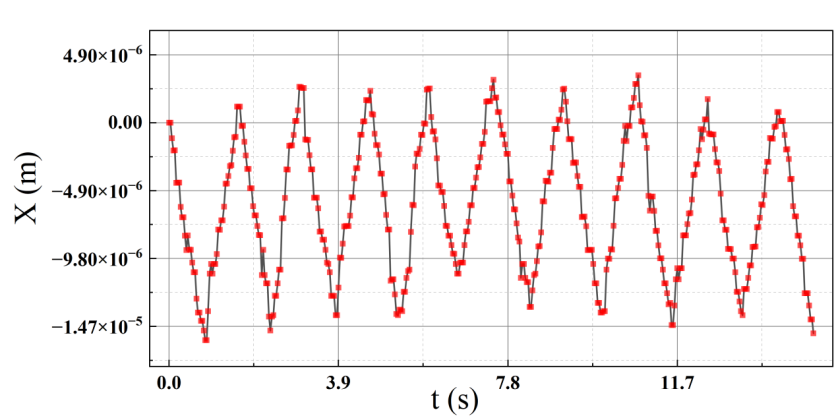
\includegraphics[width=\linewidth]{10v0.5Hz1.png}
        \caption{方波10v0.5Hz位移-时间图}
    \end{subfigure}

    \begin{subfigure}{0.25\textwidth}
        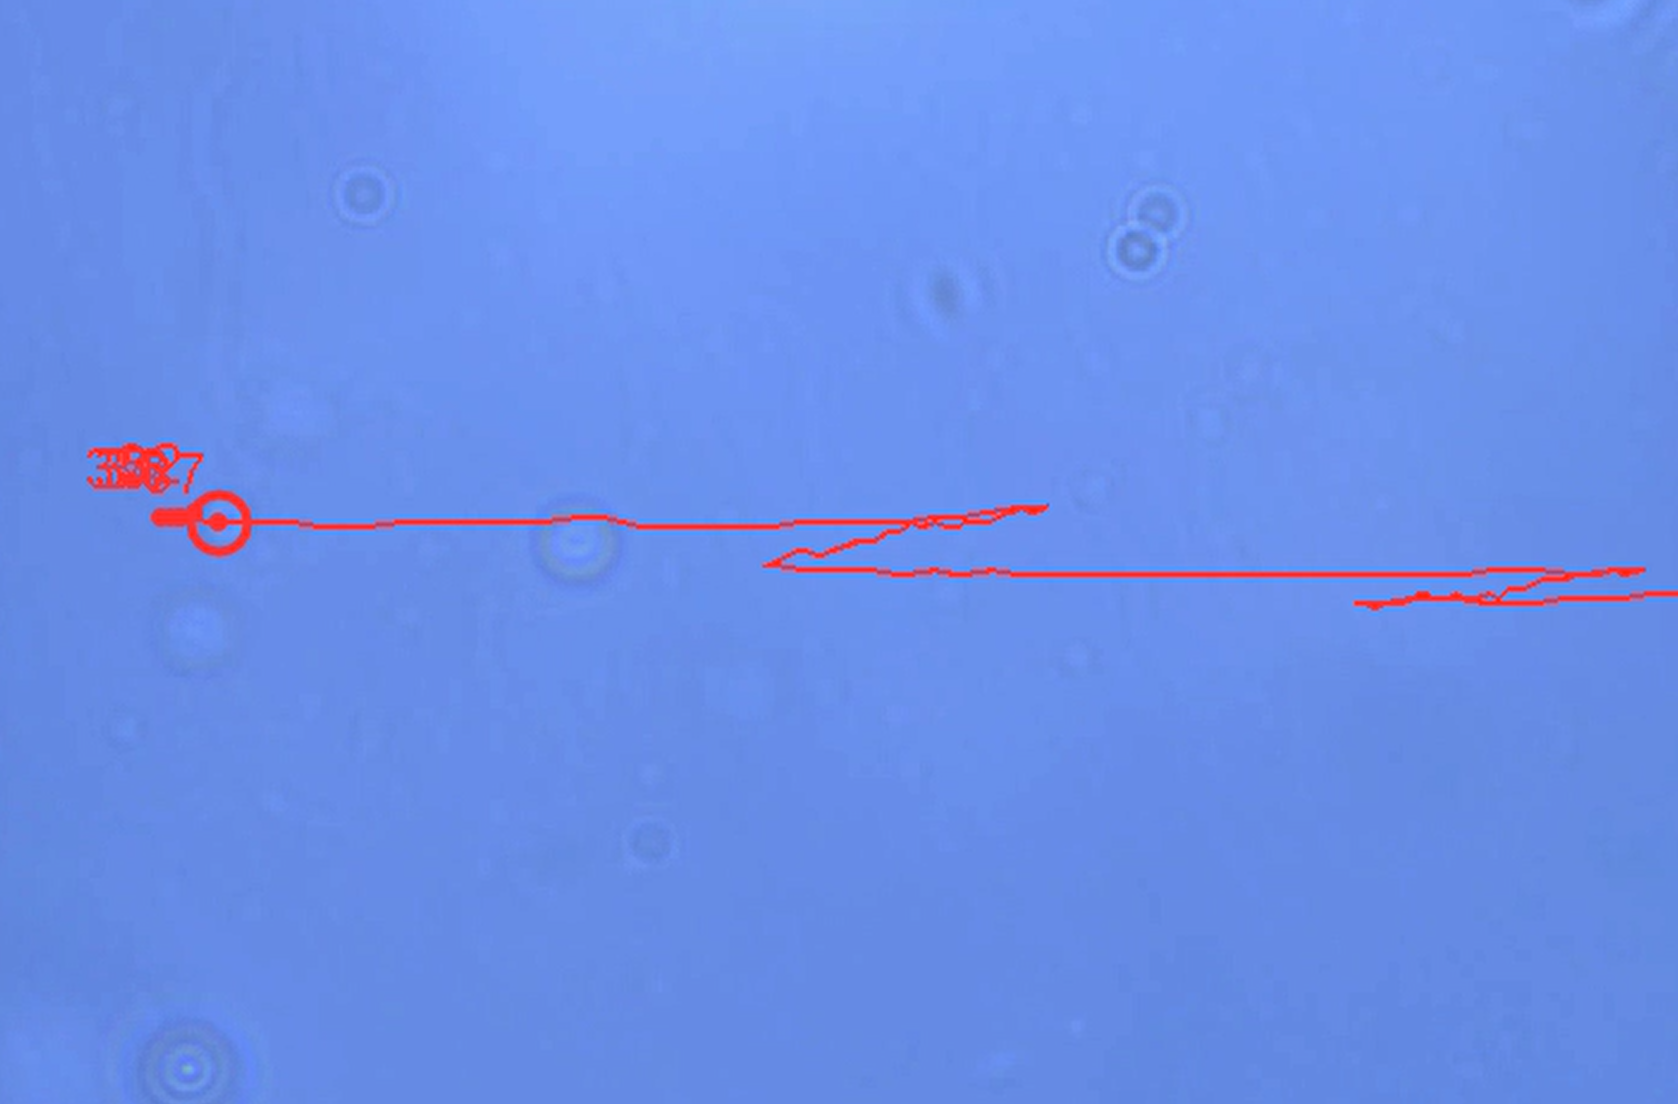
\includegraphics[width=\linewidth]{10v0.1Hz.png}
        \caption{方波10v0.1Hz轨迹图}
    \end{subfigure}
    \begin{subfigure}{0.45\textwidth}
        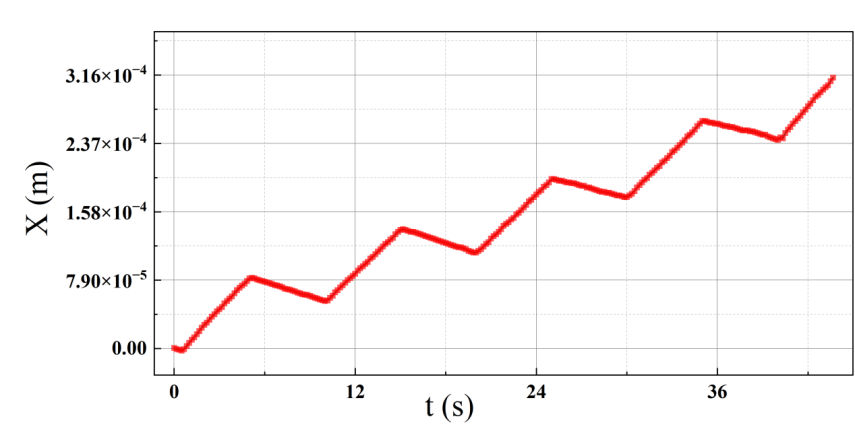
\includegraphics[width=\linewidth]{10v0.1Hz1.png}
        \caption{方波10v0.15Hz位移-时间图}
    \end{subfigure}

    \begin{subfigure}{0.25\textwidth}
        \includegraphics[width=\linewidth]{sin10v0.5Hz1.png}
        \caption{正弦波10v0.5Hz轨迹图}
    \end{subfigure}
    \begin{subfigure}{0.45\textwidth}
        \includegraphics[width=\linewidth]{sin10v0.5Hz.png}
        \caption{正弦波10v0.5Hz位移-时间图}
    \end{subfigure}

    \caption{0.5~$\mu$m的粒子在加载不同波形和频率的运动轨迹和x-t图}
\end{figure}

在实验中,我们分别设置噪声强度为0--10v,电压间隔为2v,测量了不同噪声强度下0.5~$\mu$m粒子的MSD,如图所示:\par
\begin{figure}[H]
    \centering
    \includegraphics[width=0.8\textwidth]{不同噪声强度下的MSD.png}
    \caption{不同噪声强度下的MSD}
    \label{fig:msdnoise}
\end{figure}
汇总扩散系数D拟合结果,同时根据\eqref{eq:Teff}我们也可以计算有效温度随电压的变化:
\begin{table}[H]
    \centering
    \caption{不同电压下的扩散系数对比}
    \begin{tabular}{cccc}
        \toprule
        电压 & $D$ 拟合值 (m$^2$/s) & $D$ 理论值 (m$^2$/s) & 误差 (\%) \\
        \midrule
        0V  & $9.885 \times 10^{-13}$ & $9.871 \times 10^{-13}$ & 0.14 \\
        2V  & $9.994 \times 10^{-13}$ & $9.871 \times 10^{-13}$ & 1.24 \\
        4V  & $1.010 \times 10^{-12}$ & $9.871 \times 10^{-13}$ & 2.36 \\
        6V  & $1.020 \times 10^{-12}$ & $9.871 \times 10^{-13}$ & 3.38 \\
        8V  & $1.051 \times 10^{-12}$ & $9.871 \times 10^{-13}$ & 6.52 \\
        10V & $1.075 \times 10^{-12}$ & $9.871 \times 10^{-13}$ & 8.92 \\
        \bottomrule
    \end{tabular}
\end{table}
\begin{table}[H]
    \centering
    \caption{不同电压下的动能温度与温升}
    \begin{tabular}{ccc}
        \toprule
        电压 (V) & $T_{\text{kin}}$ (K) & $\Delta T$ (K) \\
        \midrule
        0  & 300.42 & 0.42 \\
        2  & 303.73 & 3.73 \\
        4  & 306.95 & 6.95 \\
        6  & 309.99 & 9.99 \\
        8  & 319.41 & 19.41 \\
        10 & 326.71 & 26.71 \\
        \bottomrule
    \end{tabular}
\end{table}

\begin{figure}[H]
    \centering
    \includegraphics[width=0.8\textwidth]{二次拟合.png}
    \caption{扩散系数随电压的二次函数关系}
    \label{fig:trends}
\end{figure}
根据公式\eqref{eq:D_sigma},D和V之间应该满足二次关系。对D和V作图,进行$D = D_0 + kV^2$的二次拟合,得到拟合后的参数。
我们可以得知
\begin{equation}
    D = D_0 + \frac{\sigma^2}{(2\gamma)^2},
\end{equation}

对于有效温度:
\begin{equation}
    T_{\text{kin}} = T_{\omega} + \frac{\sigma^2}{2\text{k}\gamma},
\end{equation}


\begin{figure}[H]
    \centering
    \includegraphics[width=0.8\textwidth]{有效温度.png}
    \caption{有效温度随噪声电压的变化图}
    \label{fig:fit2V}
\end{figure}



\section{注意事项}
(1)每次使用完微量移液器,比色皿和电极片需要用无水乙醇清洗干净,防止污染。\par
(2)实验过程中,不要随意走动或在试验台上进行其他操作,尽量避免振动和气流对比色皿的影响。\par
(3)待每次采集微球的运动数据后,需尽快移走比色皿并保持其他部分装置不动和CCD曝光时间相同,尽快拍摄背景图片 \par
(4)在使用信号发生器加载不同幅度的噪声时,需要确保电极是紧贴着内壁两侧。且加载电压要从0v逐渐增加到10v,而不能从10v逐渐降低电压
至0v,防止微球先收到高电压的噪声未经静置而影响后续MSD的计算。\par
(5)在进行分辨率板的标定实验后,需要固定其他剩余的实验装置,尤其是100x物镜和CCD的相对位置,以保证标定分辨率板后的像素尺寸不会发生变化。\par

\chapter{结论与展望}
\section{实验结论}
本实验成功构建了一套集光学观测与电噪声操控于一体的实验系统,实现了对外加可控电噪声驱动下布朗粒子扩散行为的系统性研究。实验验证了通过电噪声调控可有效模拟"人工热浴"效应,为在常温环境下研究高温扩散特性及非平衡统计物理现象提供了创新性实验范式。主要研究成果如下:

首先,在理论层面,基于朗之万方程建立了外部噪声作用下的有效温度与扩散系数理论模型。理论推导表明,外加随机力可等效提升布朗粒子的动能温度,其贡献量与噪声强度的平方成正比,与阻尼系数成反比。
这一结论与已有研究相吻合 \cite{Martinez2013,Roldan2014},为实验中观察到的温度随电压升高现象提供了理论解释。修正后的扩散系数公式进一步揭示了外部噪声对系统弛豫行为和熵产生机制的影响 \cite{Leighton2024}。

其次,在实验系统构建方面,采用垂直样品放置设计有效避免了容器壁对微粒运动的干扰,实现对更大粒径微粒的布朗运动研究。通过非相干光源与高倍显微镜结合CCD成像的系统配置,实现了对微球布朗运动轨迹的精确捕捉。
结合信号发生器产生的0-10V可调电噪声,建立了非平衡驱动强度连续可调的实验平台。

实验结果表明:
\begin{itemize}
    \item 对不同粒径粒子与不同粘度环境下MSD数据的拟合证实,实验测得的扩散系数与理论预测高度一致,验证了 $D \propto 1/r$ 与 $D \propto 1/\eta$ 的基本关系。
    \item 在外加高斯白噪声作用下,0.5~$\mu$m微粒的MSD随电压升高呈现系统性增大趋势。通过对MSD曲线前30个数据点的线性拟合,获得了不同电压下的扩散系数,并据此计算出相应的有效温度。
    \item 扩散系数 $D$ 与电压平方 $V^2$ 呈现良好的二次函数关系,拟合参数与理论值的相对误差仅为 $1.6\%$,证实了理论模型的准确性。
    \item 有效温度的实验斜率与理论斜率的差异为 $1.9\%$,进一步验证了外部随机驱动等效加热效应的可靠性。
\end{itemize}

本实验不仅定性验证了电噪声对布朗粒子动力学的调控作用,更在定量层面通过MSD与扩散系数的精确测量,展示了理论与实验的高度一致性。研究成果为理解非平衡体系中的温度涌现机制、扩散行为调控和熵产生过程提供了实验依据,
证实了电噪声驱动平台在非平衡统计物理研究中的有效性和应用潜力,填补了大学物理实验中热学相关综合性实验的空白。

\section{未来展望}
基于本实验构建的光学-电噪声一体化实验系统及已有研究成果,未来工作可从以下几个方向深入开展:

首先,在理论探索方面,可进一步研究不同类型噪声(如有色噪声、非高斯噪声、时空关联噪声)对布朗粒子动力学的影响,系统分析噪声统计特性对有效温度、扩散行为及熵产生率的调控规律,
完善非平衡态随机热力学的理论框架。同时,可通过数值模拟研究多粒子体系和耦合系统中的集体扩散现象与能量传递机制。

其次,在实验技术方面,可引入高速摄像与三维追踪技术,提升粒子运动轨迹的时间与空间分辨率,精确测量粒子的瞬时速度分布与轨迹涨落特性,为理论模型提供更精细的实验验证。
还可开发多通道独立控制的电极阵列,实现空间局域化的噪声调控,研究噪声梯度场中的粒子输运行为。

此外,在应用拓展方面,可探索该实验系统在软物质物理、生物物理等交叉学科领域的应用,如研究外部噪声对胶体自组装、分子马达运动、细胞膜输运等过程的影响,
为生命体系中的非平衡现象研究提供新的实验手段。还可将该方法与微流控技术结合,开发基于噪声调控的微纳颗粒分离与操控技术。

最后,在教学应用方面,可进一步完善实验方案,开发成综合性物理实验课程,让学生通过亲自动手操作,深入理解布朗运动、涨落-耗散定理和非平衡统计物理等核心概念,
培养实验设计与数据分析能力,提升大学物理实验教学的前沿性与创新性。

\chapter{附录}
\section{有效拟合区间的选取(MSD 与延迟时间 $\Delta t$ 的关系分析)}
\subsection*{一、分析目的}

研究粒子运动的均方位移(Mean Squared Displacement, MSD)随延迟时间 $\Delta t$ 的变化关系,并结合理论误差模型评估测量结果的可靠性。通过绘制 MSD 曲线及其误差带,确定有效分析的时间范围(即统计误差小于 10\% 的区间),为后续扩散行为分析提供依据。

\subsection*{二、理论原理}
\subsubsection*{1. 均方位移(MSD)}
均方位移是描述粒子扩散行为的重要物理量,定义为:
\[
\text{MSD}(k) = \langle |\vec{r}(t + k\Delta t) - \vec{r}(t)|^2 \rangle
\]
其中:
\begin{itemize}
    \item $k$:延迟步数(lag time)
    \item $\Delta t$:单步时间间隔
    \item $\vec{r}(t)$:粒子在时间 $t$ 的位置
    \item $\langle \cdot \rangle$:对所有起始时间 $t$ 的平均
\end{itemize}
在正常扩散中,MSD 与 $\Delta t$ 呈线性关系:
\[
\text{MSD} \propto \Delta t
\]
\subsubsection*{2. 相对误差模型}
由于有限轨迹长度,MSD 的估计存在统计误差。定义 $\rho_k = \text{MSD}(k)$,其相对标准偏差为:
\[
\frac{\Delta \rho_k}{\langle \rho_k \rangle}
\]
根据相关文献内的理论推导\cite{qian1991spt},该比值可由以下分段函数估算:
\[
\frac{\Delta \rho_k^2}{\langle \rho_k \rangle^2} =
\begin{cases}
\displaystyle \frac{4(N-k)k^2 + 2(N-k) + k - k^3}{6k(N-k)^2}, & k < \tfrac{N}{2} \\[2ex]
\displaystyle 1 + \frac{(N-k)^3 - 4(N-k)^2 k + 5k - N}{6k^2(N-k)}, & k \geq \tfrac{N}{2},\; k < N
\end{cases}
\]
其中 $N$ 为轨迹的总帧数。

\subsubsection*{3. 有效分析范围}

设定阈值:当 
\[
\frac{\Delta \rho_k}{\langle \rho_k \rangle} < 10\%
\] 
时,认为统计误差可接受。通过计算该比值随 $k$ 的变化,确定最大有效延迟步数 $k_{\text{max}}$,对应 $\Delta t_{\text{max}}$。

\subsection*{三、数据处理流程}

\subsubsection*{1. 数据读取}

从 CSV 文件 \texttt{msd\_curve.csv} 中读取两列数据:
\begin{itemize}
    \item \texttt{delta\_t}:延迟时间 $\Delta t$(单位:秒)
    \item \texttt{MSD}:对应延迟时间下的均方位移(单位:$\mu m^2$)
\end{itemize}

\subsubsection*{2. 参数设置}

\begin{itemize}
    \item 总帧数 $N = \text{len}(\text{delta\_t})$
    \item 延迟步数 $k = 1, 2, \dots, N-1$
\end{itemize}

\subsubsection*{3. 误差比计算}

对每个 $k$ 计算 $\frac{\Delta \rho_k}{\langle \rho_k \rangle}$,并用于构建误差带:
\[
\text{上界: } \text{MSD}(k) \times \left(1 + \frac{\Delta \rho_k}{\langle \rho_k \rangle}\right)
\]
\[
\text{下界: } \text{MSD}(k) \times \left(1 - \frac{\Delta \rho_k}{\langle \rho_k \rangle}\right)
\]

\subsubsection*{4. 确定有效范围}

找到第一个满足 $\frac{\Delta \rho_k}{\langle \rho_k \rangle} \geq 0.1$ 的 $k$ 值,对应 $\Delta t$ 作为红色虚线标注。

通过上述计算模拟得到的图像可以发现:当 
\[
\frac{\Delta \rho_k}{\langle \rho_k \rangle} < 10\%
\]
时,曲线的线性关系较好(误差可以接受)的位置可以作为有效拟合区间。在本实验中我们取有效拟合区间为前 20 个数据点,即 $\Delta t \approx 1 \ \text{s}$ 附近。

\begin{figure}[H]
    \centering
    \includegraphics[width=0.9\textwidth]{取1.jpg}
    \caption{MSD与延迟时间的关系}
    \label{fig:let1}
\end{figure}
\section{实验仪器规格与人员分工}
\begin{table}[H]
\centering
\caption{成本统计表}
\begin{tabular}{c c c c}
\toprule
序号 & 类别 & 名称 & 金额 \\
\midrule
1 & \multirow{4}{*}{耗材} & 甘油 & 34 \\
2 &                     & PS微球(0.5、1、2$\mu$m) & 500 \\
3 &                     & 烧杯等器皿 & 100 \\
4 &                     & 比色皿 & 250 \\
\midrule
\multirow{3}{*}{5} & \multirow{3}{*}{电子元件} 
 & LED光源 & 20 \\
 & & MV-CS200-10UC工业相机 & 2000 \\
 & & AFG-2225信号发生器 & 1500 \\
\midrule
\multirow{2}{*}{6} & \multirow{2}{*}{显微与标定模块} 
 & 100x物镜(JCOPTIX NA=0.8 WD2) & 2450 \\
 & & USAF 1951分辨率板 & 800 \\
\midrule
\multirow{2}{*}{7} & \multirow{2}{*}{平台与支架} 
 & 光学平台 & 300 \\
 & & 光学支架 & 500 \\
\midrule
 & & 合计 & 8454 \\
\bottomrule
\end{tabular}
\end{table}

\renewcommand{\arraystretch}{1.3} % 表格行距调整

\begin{tabularx}{\textwidth}{>{\bfseries}l X}
\toprule
队员 & 分工 \\
\midrule
队员一 & 负责实验数据采集,实验报告的撰写等。 \\
队员二 & 负责热学相关部分原理的推导和微球布朗运动的模拟等。 \\
队员三 & 负责制作ppt和实验采集,查阅文献等。 \\
队员四 & 负责后期数据处理,误差分析,查阅文献等。 \\
\bottomrule
\end{tabularx}

\section{实验内容补充}
\subsection{部分使用代码}
\begin{lstlisting}[language=Python, caption=有效拟合区间的选取, label=code:calculate1]
def calculate_ratio(k, N):
    if k < N / 2:
        return (4 * (N - k) * k**2 + 2 * (N - k) + k - k**3) / (6 * k * (N - k)**2)
    else:
        return 1 + ((N - k)**3 - 4 * (N - k)**2 * k + 5 * k - N) / (6 * k**2 * (N - k))
df = pd.read_csv(r'E:\26day\500nm\msd_curve.csv')

# 提取Δt和MSD数据
delta_t = df['time_lag (s)'].values
msd_values = df['ensemble_MSD (m^2)'].values
N = len(delta_t)
k_values = np.arange(1, N)  # 1, 2, ..., N-1

# 截取前 N-1 个数据点用于绘图(因为 ratio 只能算到 N-1)
delta_t_plot = delta_t[:N-1]
msd_plot = msd_values[:N-1]

# 计算 ratio 值
ratio_values = [calculate_ratio(k, N) for k in k_values]
ratio_array = np.array(ratio_values)

# 计算误差带
error_band_upper = msd_plot * (1 + ratio_array)
error_band_lower = msd_plot * (1 - ratio_array)

# 找到第一个 ratio >= 10% 的位置
threshold_index = np.argmax(ratio_array >= 0.1)
threshold_dt = delta_t_plot[threshold_index]
\end{lstlisting}

\begin{lstlisting}[language=Python, caption=检测微球, label=code:searchforparticles]
def filter_stationary_particles(trajectories, max_displacement=2.0, min_frames=10):
    """
    过滤静止不动的粒子(CCD灰尘)
    
    参数:
    trajectories: 轨迹数据
    max_displacement: 最大允许位移(像素),小于此值认为是静止粒子
    min_frames: 最小帧数,少于这个帧数的轨迹直接过滤
    """
    
    filtered_trajectories = []
    stationary_count = 0
    short_trajectory_count = 0
    
    for particle_id, group in trajectories.groupby('particle'):
        # 过滤短轨迹
        if len(group) < min_frames:
            short_trajectory_count += 1
            continue
            
        # 计算粒子的总位移
        start_frame = group['frame'].min()
        end_frame = group['frame'].max()
        
        start_pos = group[group['frame'] == start_frame][['x', 'y']].values[0]
        end_pos = group[group['frame'] == end_frame][['x', 'y']].values[0]
        
        total_displacement = np.sqrt(np.sum((end_pos - start_pos) ** 2))
        
        # 计算RMS位移
        mean_x = group['x'].mean()
        mean_y = group['y'].mean()
        rms_displacement = np.sqrt(np.mean((group['x'] - mean_x) ** 2 + (group['y'] - mean_y) ** 2))
        
        # 过滤静止粒子
        if total_displacement < max_displacement and rms_displacement < max_displacement:
            stationary_count += 1
            continue
        
        # 保留非静止粒子
        filtered_trajectories.append(group)
    
    if filtered_trajectories:
        filtered_df = pd.concat(filtered_trajectories, ignore_index=True)
    else:
        filtered_df = pd.DataFrame(columns=trajectories.columns)
    
    print(f"过滤结果:")
    print(f"  总粒子数: {trajectories['particle'].nunique()}")
    print(f"  静止粒子数: {stationary_count}")
    print(f"  短轨迹粒子数: {short_trajectory_count}")
    print(f"  有效粒子数: {filtered_df['particle'].nunique()}")
    
    return filtered_DataFrame

def batch_detect_particles(frames, params):
    """批量检测所有帧中的粒子"""
    all_features = []
    
    print("开始批量检测粒子...")
    for i, frame in enumerate(frames):
        # 使用trackpy检测粒子
        features = tp.locate(frame, 
                            diameter=params['diameter'],
                            minmass=params['minmass'],
                            separation=params['separation'],
                            noise_size=params['noise_size'],
                            invert=params['invert'])
        
        # 添加帧编号信息
        features['frame'] = i
        all_features.append(features)
        
        if (i + 1) % 50 == 0:
            print(f"已处理 {i + 1}/{len(frames)} 帧,当前帧检测到 {len(features)} 个粒子")
    
    # 合并所有检测结果
    combined_features = pd.concat(all_features, ignore_index=True)
    print(f"\n总共检测到 {len(combined_features)} 个粒子检测结果")
    return combined_features
\end{lstlisting}
首先使用上面的代码进行粒子检测和过滤,得到干净的粒子轨迹数据。然后使用下面的代码进行粒子跟踪、可视化和统计分析。\\
\begin{lstlisting}[language=Python, caption=可视化与计算, label=code:calculate]
def track_particles(features_df, search_range=50, memory=5):
    """跟踪粒子运动轨迹"""
    print("开始粒子跟踪...")
    
    # 使用trackpy进行粒子跟踪
    trajectories = tp.link(features_df, 
                          search_range=search_range, 
                          memory=memory,
                          neighbor_strategy='KDTree')
    
    # 计算每个轨迹的粒子数量
    particle_counts = trajectories['particle'].value_counts()
    
    print(f"跟踪完成!")
    print(f"总共跟踪到 {len(particle_counts)} 个独立粒子")
    print(f"轨迹长度统计:")
    print(f"最长轨迹: {particle_counts.max()} 帧")
    print(f"最短轨迹: {particle_counts.min()} 帧")
    print(f"平均轨迹长度: {particle_counts.mean():.2f} 帧")
    
    return trajectories

def visualize_particle_movement(trajectories):
    """可视化粒子运动轨迹"""
    plt.figure(figsize=(12, 10))
    
    # 为每个粒子分配颜色
    particle_ids = trajectories['particle'].unique()
    colors = plt.cm.viridis(np.linspace(0, 1, len(particle_ids)))
    
    for i, particle_id in enumerate(particle_ids):
        group = trajectories[trajectories['particle'] == particle_id]
        if len(group) > 5:  # 只显示有足够数据的轨迹
            plt.plot(group['x'], group['y'], 'o-', 
                    markersize=2, linewidth=1, alpha=0.7, 
                    color=colors[i], label=f'粒子 {particle_id}')
    
    plt.title('粒子运动轨迹', fontsize=16, fontweight='bold')
    plt.xlabel('X坐标 (像素)', fontsize=12)
    plt.ylabel('Y坐标 (像素)', fontsize=12)
    plt.grid(True, alpha=0.3)
    plt.legend(bbox_to_anchor=(1.05, 1), loc='upper left')
    plt.tight_layout()
    plt.show()

def calculate_basic_statistics(trajectories):
    """计算基本统计信息"""
    print("\n轨迹统计信息:")
    print("=" * 40)
    
    # 轨迹长度统计
    trajectory_lengths = trajectories.groupby('particle').size()
    print(f"平均轨迹长度: {trajectory_lengths.mean():.2f} 帧")
    print(f"最长轨迹: {trajectory_lengths.max()} 帧")
    print(f"最短轨迹: {trajectory_lengths.min()} 帧")
    
    # 位移统计
    displacements = []
    for particle_id, group in trajectories.groupby('particle'):
        if len(group) > 1:
            start_pos = group[group['frame'] == group['frame'].min()][['x', 'y']].values[0]
            end_pos = group[group['frame'] == group['frame'].max()][['x', 'y']].values[0]
            displacement = np.sqrt(np.sum((end_pos - start_pos) ** 2))
            displacements.append(displacement)
    
    if displacements:
        print(f"平均位移: {np.mean(displacements):.2f} 像素")
        print(f"最大位移: {np.max(displacements):.2f} 像素")
        print(f"最小位移: {np.min(displacements):.2f} 像素")
    
    print(f"总粒子数: {trajectories['particle'].nunique()}")
    print(f"总数据点: {len(trajectories)}")
\end{lstlisting}

\subsection{实验数据}
\begin{figure}[H]
    \centering
    % 每行 2 张
    \begin{subfigure}{0.45\textwidth}
        \includegraphics[width=\linewidth]{不同比例.png}
        \caption{甘油与水不同比例}
    \end{subfigure}
    \begin{subfigure}{0.45\textwidth}
        \includegraphics[width=\linewidth]{不同电压.png}
        \caption{加载不同电压}
    \end{subfigure}

    \begin{subfigure}{0.45\textwidth}
        \includegraphics[width=\linewidth]{不同波形.png}
        \caption{加载不同波形}
    \end{subfigure}
    \begin{subfigure}{0.45\textwidth}
        \includegraphics[width=\linewidth]{不同粒子直径.png}
        \caption{不同粒子直径}
    \end{subfigure}

    \caption{实验相关数据}
\end{figure}
\begin{figure}[H]
    \centering
    % 每行 3 张
    \begin{subfigure}{0.3\textwidth}
        \includegraphics[width=\linewidth]{0.5um.png}
        \caption{0.5~$\mu$m粒子}
    \end{subfigure}
    \begin{subfigure}{0.3\textwidth}
        \includegraphics[width=\linewidth]{2um.png}
        \caption{2.0~$\mu$m粒子}
    \end{subfigure}
    \begin{subfigure}{0.3\textwidth}
        \includegraphics[width=\linewidth]{5um.png}
        \caption{5.0~$\mu$m粒子}
    \end{subfigure}

    \caption{不同直径粒子拍摄图(已转为灰度图)}
\end{figure}
\addcontentsline{toc}{chapter}{参考文献} % 手动加到目录
\bibliographystyle{plain}
\bibliography{refs}
\end{document}
